\clearpage
\begin{savequote}[8cm]
\textlatin{Neque porro quisquam est qui dolorem ipsum quia dolor sit amet, consectetur, adipisci velit...}

There is no one who loves pain itself, who seeks after it and wants to have it, simply because it is pain...
  \qauthor{--- Cicero's \textit{de Finibus Bonorum et Malorum}}
\end{savequote}

\chapter{\label{ch:5-cpfit}Fits for \CP observables in two- and four-body decays} 

\minitoc

In this section the \CP observables are measured using the yields of \btodkst in each \D decay mode for both \Bp and \Bm decays.

The setup of the \CP fit is outlined in Section \ref{sec:cpfit:setup}, followed by the fit results in Section \ref{sec:cpfit:results}. Section \ref{sec:systematics} outlines the systematic uncertainties and the results of the \CP observables are summarised in Section \ref{sec:cpfit:summary}.

\section{Setup of \CP fit}
\label{sec:cpfit:setup}

The fit to data is performed on the invariant mass of B candidates. A simultaneous fit stategy is employed to fit each of the D decay modes as well as two bins of B charge ($B^+$ and $B^-$), two bins of $K_s$ track type (LL and DD) and two bins of data type (Run 1 and Run 2), resulting in 56 bins in total.

As discussed in Section \ref{sec:massfit:range} the \CP fit is performed from 5230 MeV. The components and shapes of the \CP fit are the same as those described in Section \ref{sec:massfit}. The mean and width of the signal shape are shared across the different run periods and across modes of the same number of final state particles, but the mean and width are allowed to be different for the two- and four-body modes. The shape and yield of the partially reconstructed background is completely fixed, with different shape parameters for LL and DD candidates. The shape is fixed as described in Section \ref{sec:massfit:partreco}, using the yield ratios given in Table \ref{fixedyieldratios}. The total yield is fixed from the fits in Figures \ref{massfitskpi} and \ref{massfitsk3pi}, the values for the total partially reconstructed yield in each of the simultaneous fit categories is given in Appendix \ref{sec:app:partrecoyields}. The shape of the combinatoric background is shared across all modes of the same number of final state particles, but has different values for LL and DD candidates, as well as two and four-body D modes.

The \CP fit parameters are the \CP observables \Akpi, \Akk, \Apipi, \Rkk, \Rpipi, \Rptwo, \Rmtwo, \Akpipipi, \Apipipipi, \Rpipipipi, \Rpfour and \Rmfour, which relate to the physics parameters of interest as shown in Equations \ref{exp_Acp} - \ref{exp_R4pi}.

\subsection{Corrections to yield ratios}
\label{sec:cpfit:efficiencies}

The \CP fit measures seven observables, \Rkk, \Rpipi, \Rptwo, \Rmtwo, \Rpipipipi, \Rpfour and \Rmfour, which relate to the yield ratios with respect to \decay{\Bm}{\D(\Km\pip)\Kstarm} and \decay{\Bm}{\D(\Km\pip\pim\pip)\Kstarm} for two- and four-body observables respectively. In order to extract these \CP observables from the raw yield ratios, various efficiency corrections, taken from simulated signal samples, must be applied.

For the GLW modes, the fit takes the raw value of the yield ratio and applies efficiency corrections to extract \Rkk, \Rpipi and \Rpipipipi as shown in Equation \ref{effcorrectionglw2body} and \ref{effcorrectionglw4body}, where $\epsilon_{sel}$ and $\epsilon_{pid}$ are the selection and PID efficiencies respectively. The values for these selection and PID efficiency corrections are given in Tables \ref{seleff} and \ref{pideff} respectively.

{\footnotesize
\begin{equation}
R_{hh} = \frac{N(\decay{\Bm}{\D(h^+h^-)\Kstarm})}{N(\decay{\Bm}{\D(\Km\pip)\Kstarm})} \times \frac{\BR(\decay{\Dz}{\Km\pip})}{\BR(\decay{\Dz}{hh})} \times \frac{\epsilon_{\text{sel}}(K\pi)}{\epsilon_{\text{sel}}(hh)} \times \frac{\epsilon_{\text{pid}}(K\pi)}{\epsilon_{\text{pid}}(hh)}
\label{effcorrectionglw2body}
\end{equation}

\begin{equation}
R_{\pi\pi\pi\pi} = \frac{N(\decay{\Bm}{\D(\pip\pim\pip\pim)\Kstarm})}{N(\decay{\Bm}{\D(\Km\pip\pim\pip)\Kstarm})} \times \frac{\BR(\decay{\Dz}{\Km\pip\pim\pip})}{\BR(\decay{\Dz}{\pi\pi\pi\pi})} \times \frac{\epsilon_{\text{sel}}(K\pi\pi\pi)}{\epsilon_{\text{sel}}(\pi\pi\pi\pi)} \times \frac{\epsilon_{\text{pid}}(K\pi\pi\pi)}{\epsilon_{\text{pid}}(\pi\pi\pi\pi)} 
\label{effcorrectionglw4body}
\end{equation}}

As the final state in the ADS modes are almost identical to the corresponding charge favoured mode, the selection efficiencies that are common to both are assumed to cancel. There are only two differences between the selection for the ADS mode and the charge favoured mode; the tighter BDT selection for DD candidates and the double misID veto, which is only applied to the ADS mode. Equations \ref{effcorrectionads2body} and \ref{effcorrectionads4body} describe the effciency corrections required to extract \Rptwo, \Rmtwo, \Rpfour and \Rmfour from the raw yield ratios, where $\epsilon_{bdt}$ and $\epsilon_{veto}$ are the BDT and veto efficiencies respectively. The values for these BDT and veto efficiency corrections are given in Tables \ref{bdteff} and \ref{vetoeff} respectively.

{\footnotesize
\begin{equation}
R^{\pm}_{K\pi} = \frac{N(\decay{\Bpm}{\D(\Kmp\pipm)\Kstarpm})}{N(\decay{\Bpm}{\D(\Kpm\pimp)\Kstarpm})} \times \frac{\epsilon_{\text{bdt}}(K\pi)}{\epsilon_{\text{bdt}}(\pi K)} \times \frac{1}{\epsilon_{\text{veto}}(\pi K)}
\label{effcorrectionads2body}
\end{equation}

\begin{equation}
R^{\pm}_{K\pi\pi\pi} = \frac{N(\decay{\Bpm}{\D(\Kmp\pipm\pimp\pipm)\Kstarpm})}{N(\decay{\Bpm}{\D(\Kpm\pimp\pipm\pimp)\Kstarpm})} \times \frac{\epsilon_{\text{bdt}}(K\pi\pi\pi)}{\epsilon_{\text{bdt}}(\pi K\pi\pi)} \times \frac{1}{\epsilon_{\text{veto}}(\pi K\pi\pi)}
\label{effcorrectionads4body}
\end{equation}}

All the efficiency corrections that are used as inputs to the fit are summarised in Table \ref{fitinputs}. The final fit to the data measures $A_{K\pi}$, $A_{KK}$, $A_{\pi\pi}$, $R_{KK}$, $R_{\pi\pi}$, $R^+$,  $R^-$, $A_{K\pi\pi\pi}$, $A_{\pi\pi\pi\pi}$, $R_{\pi\pi\pi\pi}$, $R^+_{K3\pi}$ and  $R^-_{K3\pi}$, which all have the relevant efficiency corrections applied.


\subsubsection{Signal efficiencies from simulation}
\label{sec:cpfit:efficiencies:signal}

The signal efficiency of the stripping, trigger and offline selection, $\epsilon_{sel}$, is extracted from samples of simulated signal events in order to be used in Equations \ref{effcorrectionglw2body} and \ref{effcorrectionglw4body}. These values have been calculated separately for \runone and \runtwo samples as well as LL and DD categories, as shown in Table \ref{seleff}. It can be seen that the LL selection efficiency drops in \runtwo, this is thought to be due to the \KS momentum being slightly higher in \runtwo giving fewer \KS mesons decay within the \velo. PID efficiencies have not been included in these calculations; they are extracted from the {\tt PIDCalib} package~\cite{PIDCalib} and are detailed in Section \ref{sec:cpfit:efficiencies:pid}.

\begin{table}[h]
\centering
\begin{tabular}{c|cc|cc}
\hline
& \multicolumn{2}{c}{Run 1} & \multicolumn{2}{c}{Run 2} \\
& LL & DD & LL & DD \\
\hline
$\epsilon_{sel}(K\pi)$ & $0.0939 \pm 0.0011$ & $0.2519 \pm 0.0018$ & $0.1266 \pm 0.0011$ & $0.3155 \pm 0.0017$ \\
$\epsilon_{sel}(KK)$ & $0.0919 \pm 0.0011$ & $0.2450 \pm 0.0018$ & $0.1189 \pm 0.0010$ & $0.2923 \pm 0.0016$ \\
$\epsilon_{sel}(\pi\pi)$ & $0.1015 \pm 0.0012$ & $0.2584 \pm 0.0018$ & $0.1292 \pm 0.0011$ & $0.3309 \pm 0.0017$ \\
$\epsilon_{sel}(K\pi\pi\pi)$ & $0.0288 \pm 0.0006$ & $0.0816 \pm 0.0020$ & $0.0484 \pm 0.0004$ & $0.1229 \pm 0.0007$ \\
$\epsilon_{sel}(\pi\pi\pi\pi)$ & $0.0272 \pm 0.0013$ & $0.0825 \pm 0.0022$ & $0.0436 \pm 0.0011$ & $0.1185 \pm 0.0017$ \\
\hline
\end{tabular}
\caption{Summary of the selection efficiencies used in the \CP fit}
\label{seleff}
\end{table}

The BDT efficiency for the two- and four-body ADS modes is required for Equations \ref{effcorrectionads2body} and \ref{effcorrectionads4body}, which is obtained from samples of simulated signal events. The results are given in Table \ref{bdteff}.

\begin{table}[h]
\centering
\begin{tabular}{c|cc|cc}
\hline
& \multicolumn{2}{c}{Run 1} & \multicolumn{2}{c}{Run 2} \\
& LL & DD & LL & DD \\
\hline
$\epsilon_{bdt}(K\pi)$ & $0.947 \pm 0.005$ & $0.896 \pm 0.004$ & $0.949 \pm 0.003$ & $0.907 \pm 0.002$ \\
$\epsilon_{bdt}(\pi K)$ & $0.947 \pm 0.005$ & $0.802 \pm 0.005$ & $0.949 \pm 0.003$ & $0.826 \pm 0.003$ \\
$\epsilon_{bdt}(K\pi\pi\pi)$ & $0.938 \pm 0.010$ & $0.903 \pm 0.007$ & $0.952 \pm 0.003$ & $0.928 \pm 0.002$ \\
$\epsilon_{bdt}(\pi K\pi\pi)$ & $0.938 \pm 0.010$ & $0.838 \pm 0.009$ & $0.952 \pm 0.003$ & $0.870 \pm 0.003$ \\
\hline
\end{tabular}
\caption{Summary of the BDT efficiencies used in the \CP fit}
\label{bdteff}
\end{table}


\subsubsection{PID efficiencies}
\label{sec:cpfit:efficiencies:pid}

In this analysis the selection for the various \D decays modes \decay{\D}{\kaon\pi, \kaon\kaon, \pi\pi, \pi\kaon} is almost identical apart for the particle identification requirements. Therefore it is very important to apply an efficient PID selection.

As described in Section \ref{sec:selection:pid}, the PID requirements are $DLLK < 4$ for the pion from the \Kstarm and $DLLK > 2$ and $DLLK < -2$ for the \D daughters when applied to kaons and pions respectively. The efficiencies for the various selection are determined using the {\tt PIDCalib} package~\cite{PIDCalib}. The uncertainties in the PID efficiencies are systematic and come from:

%LHCb-PROC-2011-008 ; CERN-LHCb-PROC-2011-008

\begin{itemize}
\item The use of finite samples of \Dstar calibration tracks
\item The use of finite signal track samples
\item The {\tt PIDCalib} procedure
\end{itemize}

The PID efficiencies are calculated individually for each year of data-taking and each magnet polarity. They are combined separately for \runone and \runtwo according to the efficiency corrected yields in each of the samples, to be used in the \CP fit as described in Equations \ref{effcorrectionglw2body} and \ref{effcorrectionglw4body}. The results of the PID efficienies are given in Table \ref{pideff}.

\begin{table}[h]
\centering
\begin{tabular}{c|cc|cc}
\hline
& \multicolumn{2}{c}{Run 1} & \multicolumn{2}{c}{Run 2} \\
& LL & DD & LL & DD \\
\hline
$\epsilon_{pid}(K\pi)$ & $0.734 \pm 0.002$ & $0.747 \pm 0.002$ & $0.811 \pm 0.002$ & $0.821 \pm 0.002$ \\
$\epsilon_{pid}(KK)$ & $0.812 \pm 0.002$ & $0.825 \pm 0.002$ & $0.844 \pm 0.002$ & $0.853 \pm 0.002$ \\
$\epsilon_{pid}(\pi\pi)$ & $0.670 \pm 0.002$ & $0.676 \pm 0.002$ & $0.779 \pm 0.002$ & $0.790 \pm 0.002$ \\
$\epsilon_{pid}(K\pi\pi\pi)$ & $0.630 \pm 0.002$ & $0.636 \pm 0.002$ & $0.784 \pm 0.002$ & $0.798 \pm 0.002$ \\
$\epsilon_{pid}(\pi\pi\pi\pi)$ & $0.675 \pm 0.002$ & $0.687 \pm 0.002$ & $0.822 \pm 0.002$ & $0.835 \pm 0.002$ \\
\hline
\end{tabular}
\caption{Summary of the PID efficiencies used in the \CP fit}
\label{pideff}
\end{table}

Another input to the fit is the efficiency of the double misID veto, which is required as a correction to the ADS observables, as in Equations \ref{effcorrectionads2body} and \ref{effcorrectionads4body}. Veto efficiencies calculated from data are used in the \CP fit for both two- and four-body modes, given in Table \ref{vetoeff}.

\begin{table}[h]
\centering
\begin{tabular}{c|cc|cc}
\hline
& \multicolumn{2}{c}{Run 1} & \multicolumn{2}{c}{Run 2} \\
& LL & DD & LL & DD \\
\hline
$\epsilon_{veto}(\pi K)$ & $0.905 \pm 0.009$ & $0.919 \pm 0.005$ & $0.915 \pm 0.007$ & $0.917 \pm 0.004$ \\
$\epsilon_{veto}(\pi K \pi\pi)$ & $0.895 \pm 0.005$ & $0.882 \pm 0.003$ & $0.916 \pm 0.003$ & $0.906 \pm 0.002$ \\
\hline
\end{tabular}
\caption{Summary of the veto efficiencies used in the \CP fit}
\label{vetoeff}
\end{table}

It can be seen from Table \ref{pideff} that the PID efficiency in \runtwo is higher than \runone for the PID selection used in this analysis. In order to check that the PID selection for \runone is suitable to be applied to \runtwo the misID efficiency (efficiency of a $K\pi$ candidate passing the $\pi K$ PID selection) was investigated. For the two-body mode, both the PID efficiency and misID efficiency is improved in \runtwo compared to \runone so the same PID selection can be applied to both datasets. For the four-body mode the misID efficiency is slightly worse in \runtwo compared to \runone. A low misID rate is required to reduce the crossfeed background discussed in Section \ref{sec:backgrounds:crossfeed}, which reports a negligible level of this crossfeed background in both \runone and \runtwo, therefore the misID rate is already sufficiently low and so the PID selection does not need to be tightened for \runtwo.

\subsubsection{Summary of efficiency corrections}
\label{sec:cpfit:efficiencies:summary}

The \CP fit uses signal efficiencies, BDT efficiencies, PID efficiencies and double misID veto efficiencies from simulation, as well as branching ratios from Ref~\cite{PDG2016}. Table \ref{fitinputs} summarises the values used in the \CP fit. 

\begin{table}[h]
\centering
\begin{tabular}{c|cc|cc}
\hline
& \multicolumn{2}{c}{Run 1} & \multicolumn{2}{c}{Run 2} \\
& LL & DD & LL & DD \\
\hline
$BF(\decay{\Dz}{\Km\pip})$ & \multicolumn{4}{c}{$0.0393 \pm 0.0004$} \\
$BF(\decay{\Dz}{\Kp\Km})$ & \multicolumn{4}{c}{$0.00401 \pm 0.00007$} \\
$BF(\decay{\Dz}{\pip\pim})$ & \multicolumn{4}{c}{$0.001421 \pm 0.000025$} \\
$\epsilon_{sel}(K\pi)$ & $0.0939 \pm 0.0011$ & $0.2519 \pm 0.0018$ & $0.1266 \pm 0.0011$ & $0.3155 \pm 0.0017$ \\
$\epsilon_{sel}(KK)$ & $0.0919 \pm 0.0011$ & $0.2450 \pm 0.0018$ & $0.1189 \pm 0.0010$ & $0.2923 \pm 0.0016$ \\
$\epsilon_{sel}(\pi\pi)$ & $0.1015 \pm 0.0012$ & $0.2584 \pm 0.0018$ & $0.1292 \pm 0.0011$ & $0.3309 \pm 0.0017$ \\
$\epsilon_{pid}(K\pi)$ & $0.734 \pm 0.002$ & $0.747 \pm 0.002$ & $0.811 \pm 0.002$ & $0.821 \pm 0.002$ \\
$\epsilon_{pid}(KK)$ & $0.812 \pm 0.002$ & $0.825 \pm 0.002$ & $0.844 \pm 0.002$ & $0.853 \pm 0.002$ \\
$\epsilon_{pid}(\pi\pi)$ & $0.670 \pm 0.002$ & $0.676 \pm 0.002$ & $0.779 \pm 0.002$ & $0.790 \pm 0.002$ \\
$\epsilon_{bdt}(K\pi)$ & $0.947 \pm 0.005$ & $0.896 \pm 0.004$ & $0.949 \pm 0.003$ & $0.907 \pm 0.002$ \\
$\epsilon_{bdt}(\pi K)$ & $0.947 \pm 0.005$ & $0.802 \pm 0.005$ & $0.949 \pm 0.003$ & $0.826 \pm 0.003$ \\
$\epsilon_{veto}(\pi K)$ & $0.905 \pm 0.009$ & $0.919 \pm 0.005$ & $0.915 \pm 0.007$ & $0.917 \pm 0.004$ \\
$\epsilon_{sel}(K\pi\pi\pi)$ & $0.0288 \pm 0.0006$ & $0.0816 \pm 0.0020$ & $0.0484 \pm 0.0004$ & $0.1229 \pm 0.0007$ \\
$\epsilon_{sel}(\pi\pi\pi\pi)$ & $0.0272 \pm 0.0013$ & $0.0825 \pm 0.0022$ & $0.0436 \pm 0.0011$ & $0.1185 \pm 0.0017$ \\
$\epsilon_{pid}(K\pi\pi\pi)$ & $0.630 \pm 0.002$ & $0.636 \pm 0.002$ & $0.784 \pm 0.002$ & $0.798 \pm 0.002$ \\
$\epsilon_{pid}(\pi\pi\pi\pi)$ & $0.675 \pm 0.002$ & $0.687 \pm 0.002$ & $0.822 \pm 0.002$ & $0.835 \pm 0.002$ \\
$\epsilon_{bdt}(K\pi\pi\pi)$ & $0.938 \pm 0.010$ & $0.903 \pm 0.007$ & $0.952 \pm 0.003$ & $0.928 \pm 0.002$ \\
$\epsilon_{bdt}(\pi K\pi\pi)$ & $0.938 \pm 0.010$ & $0.838 \pm 0.009$ & $0.952 \pm 0.003$ & $0.870 \pm 0.003$ \\
$\epsilon_{veto}(\pi K \pi\pi)$ & $0.895 \pm 0.005$ & $0.882 \pm 0.003$ & $0.916 \pm 0.003$ & $0.906 \pm 0.002$ \\
\hline
\end{tabular}
\caption{Table of branching fractions and efficiencies used in the \CP fit. Branching ratios are taken from the PDG~\cite{PDG2016}. All these values are fixed inputs and systematics are assigned based on the uncertainties, as detailed in Section \ref{sec:systematics}.}
\label{fitinputs}
\end{table}

\subsection{Partially reconstructed yield in \CP fit}
\label{sec:cpfit:partrecoyields}

\minitoc

Table \ref{partrecofixedyields} shows the fixed values of the total partially reconstructed yield in the \CP fit.

\begin{table}[h]
\centering
\begin{tabular}{c|cc|cc}
\hline
& \multicolumn{2}{c}{Run 1} & \multicolumn{2}{c}{Run 2} \\
& LL & DD & LL & DD \\
\hline
$K\pi$ & 0.55 & 1.03 & 1.18 & 1.35 \\
$KK$ & 0.060 & 0.112 & 0.116 & 0.131 \\
$\pi\pi$ & 0.019 & 0.034 & 0.041 & 0.049 \\
$\pi K$ & 0.008 & 0.012 & 0.017 & 0.016 \\
$K\pi\pi\pi$ & 0.34 & 0.52 & 0.55 & 1.31 \\
$\pi\pi\pi\pi$ & 0.031 & 0.045 & 0.050 & 0.122  \\
$\pi K\pi\pi$ & 0.004 & 0.006 & 0.007 & 0.014 \\
\hline
\end{tabular}
\caption{Partially reconstructed yields fixed in the \CP fit. The values show \Bp and \Bm combined, therefore half of the number shown is the fixed yield in the \Bp and \Bm categories separately. Uncertainties for these values are O(10\%)}
\label{partrecofixedyields}
\end{table}


\subsection{Corrections to asymmetries}
\label{sec:cpfit:asymmetries}

For the \CP fit, the data is split by charge in order to measure various asymmetries, namely $A_{K\pi}$, $A_{KK}$, $A_{\pi\pi}$ and $A_{\pi\pi\pi\pi}$. Each observed asymmetry in the data fit is composed of \Bpm production asymmetry and detector asymmetry as well as the physics asymmetry due to \CP violation effects, which is the value to be measured. There is also a contribution from the PID asymmetry, where the PID efficiencies will be slightly different for \Bp and \Bm tracks. These asymmetries are combined as in Equation \ref{asymmetries}.

\begin{equation}
A_{raw} = A_{phys} + A_{prod} + A_{det} + A_{pid}
\label{asymmetries}
\end{equation} 

where $A_{phys}$ is the physics \CP asymmetry, $A_{prod}$ is the production asymmetry, $A_{det}$ is the detection asymmetry, $A_{pid}$ is the PID asymmetry and $A_{raw}$ is the raw measured asymmetry from the data.

The production asymmetry, detector asymmetry and PID asymmetry are corrected such that the observed asymmetry in the data fit provides a direct measurement of the physics asymmetry of interest.

\subsubsection{Production asymmetry}

The \Bpm production asymmetry is estimated using the measurements of production asymmetries in Run 1, binned in $p$ and $\eta$~\cite{LHCb-PAPER-2016-054}. The production asymmetry is calculated performing a weighted average based on the $p$ and $\eta$ distribution in the signal MC for this analysis. The value obtained is $(-0.61 \pm 0.97) \times 10^{-2}$ for 2011 data and $(-0.52 \pm 0.64) \times 10^{-2}$ for 2012 data. This gives a combined Run 1 value of $(-0.54 \pm 0.54) \times 10^{-2}$, the error will be applied as a systematic. The equivalent results for Run 2 data are not available, as such the production asymmetry for Run 2 is taken to have the same central value with twice the error being applied for the systematic, $(-0.54 \pm 1.08) \times 10^{-2}$.

\subsubsection{Detection asymmetry}

The detection asymmetry arises from differences of matter and antimatter particles as they travel through the detector. The pion detection asymmetry has been measured at LHCb at $(0.08 \pm 0.30)\%$~\cite{pi_det_asym}. However, for the kaon asymmetry the best measured value at LHCb is not $A_K$, but $A_{K\pi}$, where $A_{K\pi} = A_K - A_{\pi}$. The $K\pi$ asymmetry is calculated performing a weighted average based on the kaon momentum distribution in the signal MC. The value of $A_{K\pi}$ obtained is $(-1.06 \pm 0.16)\%$~\cite{k_det_asym}. The overall detection asymmetry in the different decay modes depends on the number of charged kaons and pions in the final state, as well as the \CP observable being measured. Table \ref{detectionasymmetry} summarises the different detection asymmetry factors that apply to each observable in the fit. The uncertainties will be applied as a systematic.

{\footnotesize
\begin{table}[h]
\begin{tabular}{cccc}
\hline
Observable & Mode & Detection asymmetry & In terms of $A_{K\pi}$ \\
\hline
$A_{K\pi}$ & $B^{\pm} \to [K^{\pm}\pi^{\mp}]_D[K_s^0\pi^{\pm}]_{K^*}$ & $A_K - A_{\pi} + A_{\pi}$ & $A_{K\pi} + A_{\pi}$ \\
$A_{KK}$ & $B^{\pm} \to [K^{\pm}K^{\mp}]_D[K_s^0\pi^{\pm}]_{K^*}$ & $A_K - A_K + A_{\pi}$ & $A_{\pi}$ \\
$A_{\pi\pi}$ & $B^{\pm} \to [\pi^{\pm}\pi^{\mp}]_D[K_s^0\pi^{\pm}]_{K^*}$ & $A_{\pi} - A_{\pi} + A_{\pi}$ & $A_{\pi}$ \\
$R_{K\pi}^+$ & $B^+ \to [K^-\pi^+]_D[K_s^0\pi^+]_{K^*}$ & $\epsilon_{K^+\pi^-}/\epsilon_{K^-\pi^+}$ & $2A_{K\pi} + 1$ \\
$R_{K\pi}^-$ & $B^- \to [K^+\pi^-]_D[K_s^0\pi^-]_{K^*}$ & $\epsilon_{K^-\pi^+}/\epsilon_{K^+\pi^-}$ & $1/(2A_{K\pi} - 1)$ \\
$A_{K\pi\pi\pi}$ & $B^{\pm} \to [K^{\pm}\pi^{\mp}\pi^{\pm}\pi^{\mp}]_D[K_s^0\pi^{\pm}]_{K^*}$ & $A_K - A_{\pi} + A_{\pi} - A_{\pi} + A_{\pi}$  & $A_{K\pi} + A_{\pi}$ \\
$A_{\pi\pi\pi\pi}$ & $B^{\pm} \to [\pi^{\pm}\pi^{\mp}\pi^{\pm}\pi^{\mp}]_D[K_s^0\pi^{\pm}]_{K^*}$ & $A_{\pi} - A_{\pi} + A_{\pi} - A_{\pi} + A_{\pi}$ & $A_{\pi}$ \\
$R_{K\pi\pi\pi}^+$ & $B^+ \to [K^-\pi^+\pi^-\pi^+]_D[K_s^0\pi^+]_{K^*}$ & $\epsilon_{K^+\pi^-}/\epsilon_{K^-\pi^+}$ & $2A_{K\pi} + 1$ \\
$R_{K\pi\pi\pi}^-$ & $B^- \to [K^+\pi^-\pi^+\pi^-]_D[K_s^0\pi^-]_{K^*}$ & $\epsilon_{K^-\pi^+}/\epsilon_{K^+\pi^-}$ & $1/(2A_{K\pi} - 1)$ \\
\hline
\end{tabular}
\caption{Detection asymmetry factors for each of the observables in the \CP fit}
\label{detectionasymmetry}
\end{table}}

\subsubsection{PID asymmetry}

The PID asymmetry arises from the asymmetry of the detector. It manifests itself in a difference between PID efficiency for positvely and negatively charged particles. Tables \ref{bachpidBminus} and \ref{bachpidBplus} show the bachelor PID efficiency in the $K\pi$ mode for each year, \KS track type and magnet polarity. The values are combined for Run 1 and Run 2, weighted by the efficiency corrected yields in each sample. The PID asymmetry $A_{pid}$, defined as,

\begin{equation*}
A_{pid} = \frac{\epsilon_{\pi^-}^{pid} - \epsilon_{\pi^+}^{pid}}{\epsilon_{\pi^-}^{pid} + \epsilon_{\pi^+}^{pid}}
\end{equation*}

is caluclated to be $(-9.56 \pm 0.19) \times 10^{-4}$ for Run 1 and $(-1.40 \pm 0.05) \times 10^{-4}$ for Run 2. These values are included in the fit as a correction to the raw asymmetry. The uncertainties will be applied as a systematic.

{\footnotesize
\begin{table}[h]
\centering
\begin{tabular}{c|cc|cc}
\hline
& \multicolumn{2}{c}{MagDown} & \multicolumn{2}{c}{MagUp} \\
& LL & DD & LL & DD \\
\hline
2011 & $94.1781 \pm 0.007$ & $95.1257 \pm 0.0034$ & $94.3937 \pm 0.0083$ & $94.8994 \pm 0.004$ \\
2012 & $95.086 \pm 0.0048$ & $95.6587 \pm 0.0065$ & $94.704 \pm 0.014$ & $95.2391 \pm 0.0016$ \\
2015 & $97.8299 \pm 0.0029$ & $97.7307 \pm 0.0017$ & $98.0431 \pm 0.0039$ & $97.8097 \pm 0.002$ \\
2016 & $97.7678 \pm 0.0031$ & $97.6973 \pm 0.0018$ & $98.1126 \pm 0.0018$ & $97.91574 \pm 0.00093$ \\
\hline
Run 1 combined & \multicolumn{4}{c}{$95.004 \pm 0.003$} \\
Run 2 combined & \multicolumn{4}{c}{$97.9145 \pm 0.0008$} \\
\hline
\end{tabular}
\caption{PID efficiency of the bachelor pion for $B^-$ tracks}
\label{bachpidBminus}
\end{table}

\begin{table}[h]
\centering
\begin{tabular}{c|cc|cc}
\hline
& \multicolumn{2}{c}{MagDown} & \multicolumn{2}{c}{MagUp} \\
& LL & DD & LL & DD \\
\hline
2011 & $94.9503 \pm 0.0056$ & $94.893 \pm 0.003$ & $94.3573 \pm 0.0072$ & $95.0011 \pm 0.003$ \\
2012 & $95.2161 \pm 0.0033$ & $95.888 \pm 0.0023$ & $95.0666 \pm 0.004$ & $95.2721 \pm 0.0017$ \\
2015 & $98.0043 \pm 0.0024$ & $97.8299 \pm 0.0015$ & $97.9034 \pm 0.0031$ & $97.8799 \pm 0.002$ \\
2016 & $97.9242 \pm 0.0027$ & $97.7934 \pm 0.0016$ & $97.9803 \pm 0.0014$ & $97.98793 \pm 0.00091$ \\
\hline
Run 1 combined & \multicolumn{4}{c}{$95.1860 \pm 0.0013$} \\
Run 2 combined & \multicolumn{4}{c}{$97.9420 \pm 0.0007$} \\
\hline
\end{tabular}
\caption{PID efficiency of the bachelor pion for $B^+$ tracks}
\label{bachpidBplus}
\end{table}}

\subsection{Likelihood function}
\label{sec:cpfit:likelihood}

The fit is performed by constructing a likelihoood function that is to be minimised. A likelihood is assigned to each candidate in a given category by constructing the signal and background PDFs. The total log-likelihood is the sum of the log-likelihoods for each of the different categories.

\begin{equation}
\log\mathcal{L} = \sum_{\Bp,\Bm}\sum_{\text{LL,DD}}\mathop{\sum_{\text{Run 1,}}}_{\text{Run 2}} \left( \log\mathcal{L}_{\D\Kstar}^{\text{2-body}} + \log\mathcal{L}_{\D\Kstar}^{\text{4-body}} \right)
\end{equation}

The expression $\log\mathcal{L}_{\D\Kstar}^{\text{2-body}}$ consists of the sum of the log likelihoods for each of the two-body modes, and equivalently for $\log\mathcal{L}_{\D\Kstar}^{\text{4-body}}$. The likelihood for each mode is constructed from the signal, combinatorial and partially reconstructed PDFs, namely $P_{\text{sig}}$, $P_{\text{comb}}$ and $P_{\text{\Dstar\Kstar}}$, respectively, with coresponding yields $N_{\text{sig}}$, $N_{\text{comb}}$ and $N_{\text{\Dstar\Kstar}}$. The two- and four-body log-likelihoods are slightly different due to the different shapes of the signal and combinatorial PDFs. The log-likelihood is given by,

\begin{equation}
\log\mathcal{L}_{\D\Kstar}^{\text{(2/4)-body}} = \mathop{\sum_{\text{(2/4)-body}}}_{\text{modes}} \log\left(N_{\text{sig}}P_{\text{sig}}^{\text{(2/4)-body}} + N_{\text{comb}}P_{\text{comb}}^{\text{(2/4)-body}} + N_{\text{\Dstar\Kstar}}P_{\text{\Dstar\Kstar}}\right) \text{ .}
\label{likelihood}
\end{equation}

The likelihood for  the \decay{\Dz}{\Kp\Km} mode has an additional $N_{\Lambda}P_{\Lambda}$ term from the $\decay{\Lb}{\Lc\Kstar}$ background, discussed in Section \ref{sec:backgrounds:Lb2LcKst}.

The signal yield $N_{\text{sig}}$ in each category is not calculated directly, but from the total signal yield for all categories in the \decay{\Dz}{\Km\pip} mode and the \CP observables.

\subsection{Fitter bias in \CP fit}
\label{sec:cpfit:fitterbias}

Data was generated according to the model described in Section \ref{sec:massfit}, using the yields taken from the single data fits to the favoured two- and four-body modes and \CP parameters were estimated assuming values of $r_B = 0.1$, $\delta_B = 111^o$ and $\gamma = 70^o$. The generated data was then fitted back using the same model and the fit parameters were extracted. This process was repeated 1000 times. The quality of the fit is tested by observing the pull distribution of each fit parameter $x$, which is given by,

\begin{equation*}
P_x = \begin{cases}
	\frac{x_{fit} - x_{gen}}{\sigma_x^-}, & \text{if $x_{fit} - x_{gen} >$ 0}. \\
	\frac{x_{gen} - x_{fit}}{\sigma_x^+}, & \text{if $x_{fit} - x_{gen} <$ 0}.
	\end{cases}
\end{equation*}

where $x_{fit}$ is the value of the parameter returned by the fit, $x_{gen}$ is the generated value of the parameter, and $\sigma_x^+$ and $\sigma_x^-$ are the upper and lower asymmetric errors respectively. The results of the pull distributions for the \CP observables are shown in Figures \ref{pulls1} and \ref{pulls2}. All pull distributions are consistent with a mean of zero and width of 1, therefore, the fit is considered stable and unbiased.
 
\begin{figure}[!h]
\centering
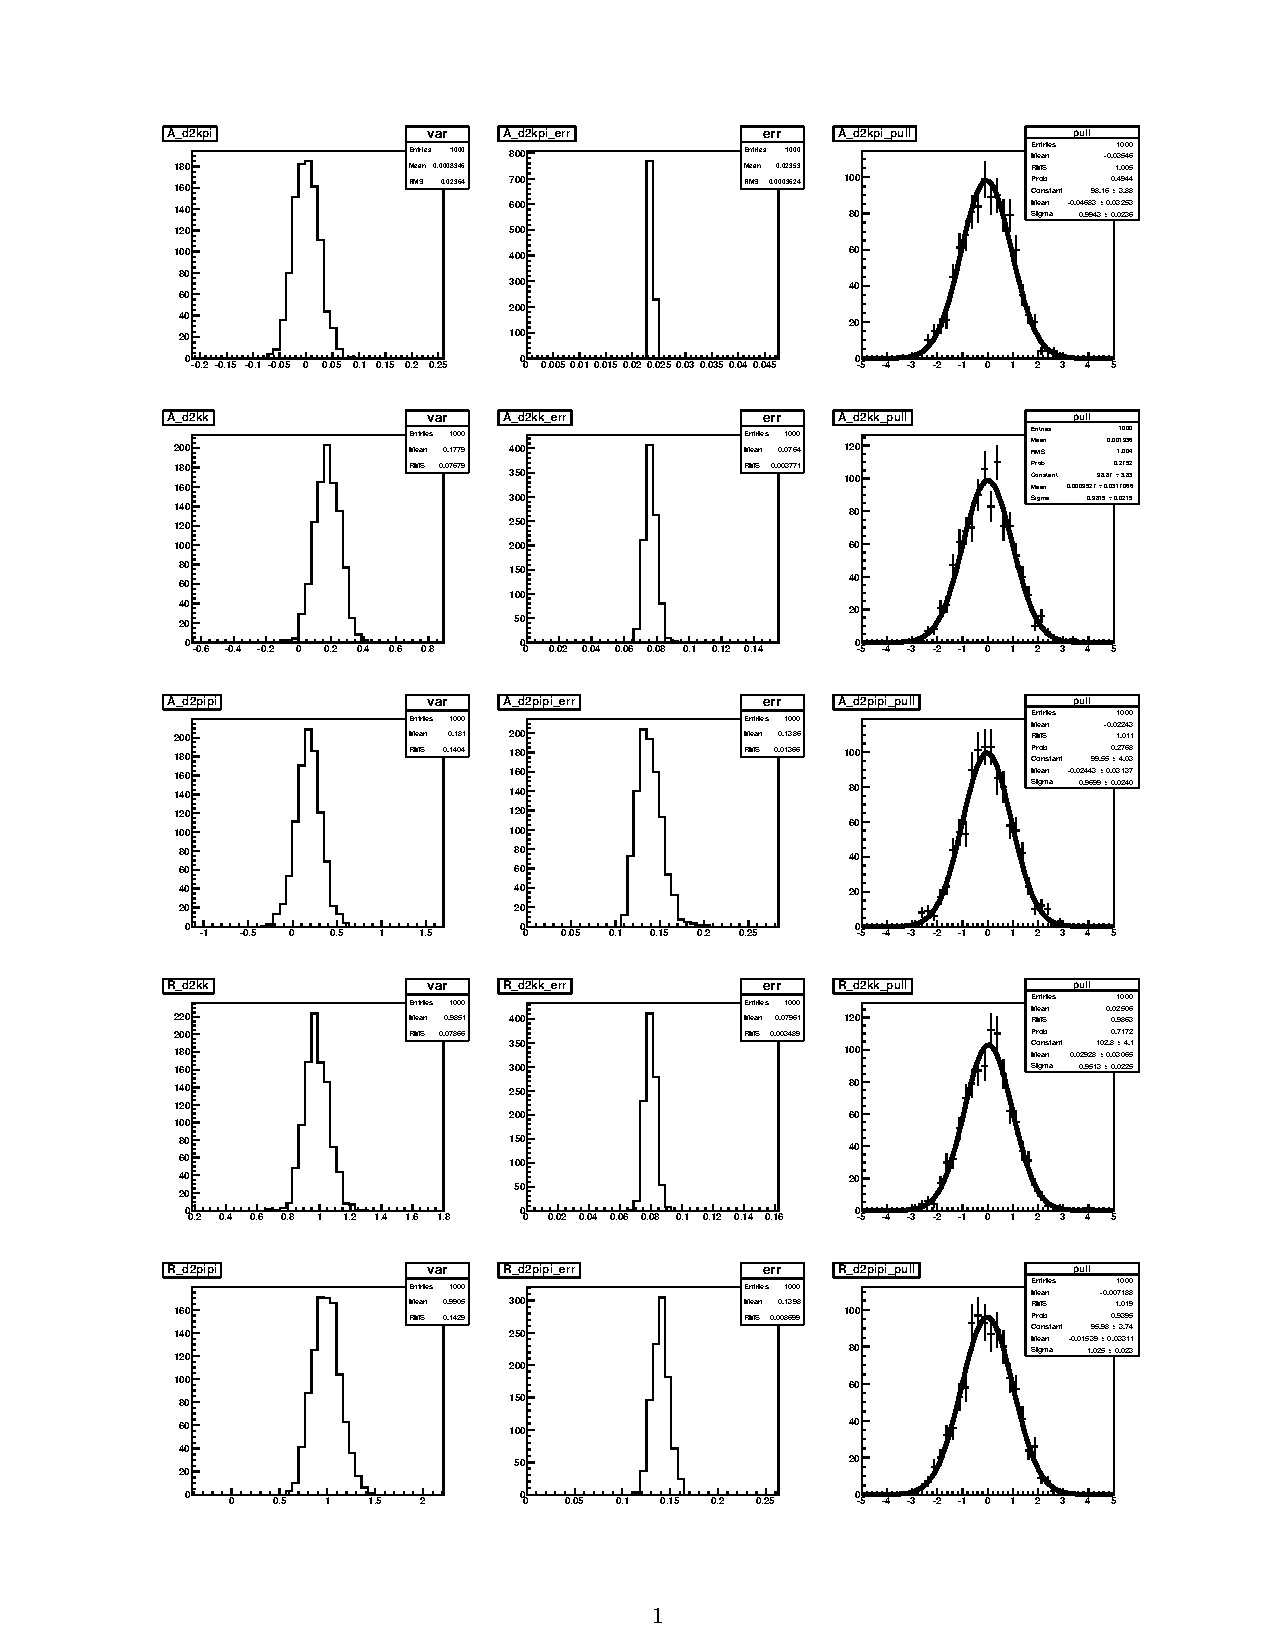
\includegraphics[page=1,trim = 0mm 24mm 0mm 0mm,clip,width=0.85\linewidth]{figures/results/toys.pdf}
\includegraphics[page=2,trim = 0mm 165mm 0mm 15mm,clip,width=0.85\linewidth]{figures/results/toys.pdf}
\caption{Pulls of the physics observables in the fit. The left hand column shows the fitted parameter distribution, the middle shows the fit error distribution and the right most plots are the pull distributions fitted with a Gaussian.}
\label{pulls1}
\end{figure}

\begin{figure}[!h]
\centering
\includegraphics[page=2,trim = 0mm 24mm 0mm 113mm,clip,width=0.85\linewidth]{figures/results/toys.pdf}
\includegraphics[page=3,trim = 0mm 165mm 0mm 15mm,clip,width=0.85\linewidth]{figures/results/toys.pdf}
\caption{Pulls of the physics observables in the fit. The left hand column shows the fitted parameter distribution, the middle shows the fit error distribution and the right most plots are the pull distributions fitted with a Gaussian.}
\label{pulls2}
\end{figure}

\subsection{Optimisation of BDT and \Kstar selection using toys}
\label{sec:cpfit:optimisation}

The BDT selection, \Kstar mass window and \KS helicity selection were optimised simultaneously with the aim of minimising the uncertainty on the \CP parameters, \Akpi, \Akk, \Apipi, \Rkk, \Rpipi, \Rptwo, \Rmtwo, \Akpipipi, \Apipipipi, \Rpipipipi, \Rpfour and \Rmfour. The selection was applied to data with no \Kstar selection and a loose ($>-0.8$) BDT selection. A single fit was performed to the two- and four-body favoured modes, as in Section \ref{sec:massfit:fit}, to give the expected signal, combinatoric and partially reconstructed yields. The signal and background efficiencies were calculated, from simulations and data, for the various selctions explored:

\begin{itemize}
\item{\Kstar mass window: 100, 75 and 50 MeV}
\item{\textbar cos(\KS helicity angle) \textbar : 0, 0.1, 0.2, 0.3 and 0.4}
\item{BDT selection: -0.8, -0.6, -0.4, -0.2, 0, 0.2, 0.4, 0.6, 0.7, 0.8, 0.9, 0.95}
\end{itemize}

Using the initial yields and efficiencies from simulation, the estimated yields for the various selections were calculated. Pseudoexperiments were generated with the expected yields and efficiencies. For the signal yield, the favoured mode was estimated from the data fit and the yield ratios and asymmetries were inferred from physics parameters using Equations \ref{exp_Acp}, \ref{exp_Rcp} and \ref{exp_Rpm}. For this optimisation process values of $r_B = 0.1$, $\delta_B = 150^{\circ}$ and $\gamma = 70^{\circ}$ were assumed. The value for \Pgamma is taken from the central value of the current \lhcb combination and $r_B$ is assumed to be the same as for \decay{\B}{\D\kaon}. A value of $\delta_B$ is chosen to be similar to values from previous analysis, although the value is completely unknown. The optimisation was repeated for various values of $\delta_B$ and it was found that the choice of selection is not sensitive to $\delta_B$.

Pseudoexperiments were performed for different selections to calculate the fit uncertainty for each selection. The fit uncertainty was taken to be the mean of the uncertainty distribution. For optimising the selection for the GLW modes, the fit error was minimised for $A_{KK}$, $R_{KK}$, $A_{\pi\pi}$ and $R_{\pi\pi}$. Figure \ref{optimisation} shows an example of the optimisation studies performed. The BDT selection for the ADS modes was optimised to minimise the fit errors in $R^+$ and $R^-$. Studies were performed to investigate a tighter BDT cut for the ADS mode as illustrated in Figure \ref{adsoptimisation}. The tighter BDT cut for DD candidates was chosen as it resulted in a lower uncertainty on $R^+$ and $R^-$ due to a reduction in the background rejection from 7\% to 2\% while retaining 80\% of the signal. In cases when the figure of merits in these optimisation studies were not especially sensitive to changes in the selection, the selection giving the highest coherence was chosen. For the BDT selection the signal and background efficiencies were taken into account.

\begin{figure}
\centering
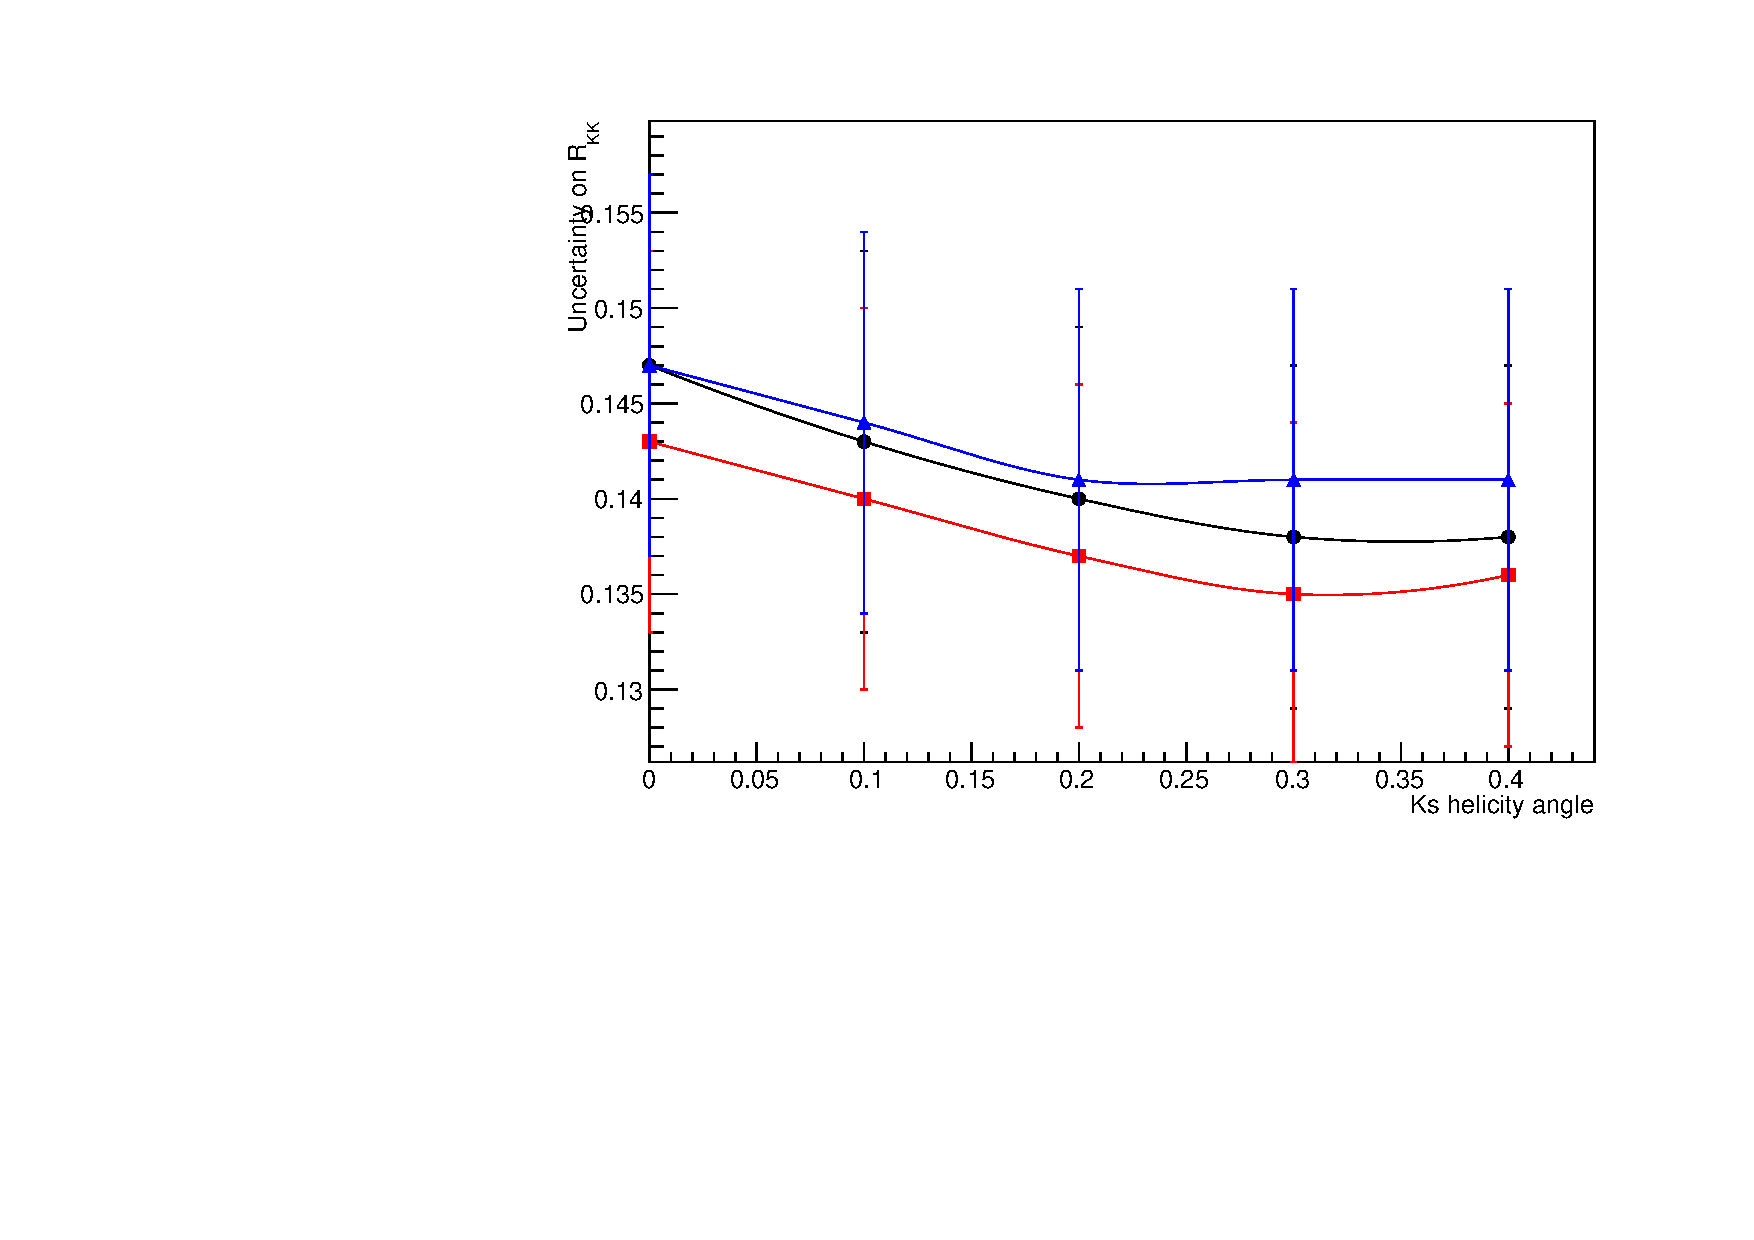
\includegraphics[width=0.8\linewidth]{figures/selection/optimisation.pdf}
\caption{Value of the uncertainty on $R_{KK}$ as a function of \KS helicity angle selection for different \Kstar mass selections. The black curve is using a \Kstar mass window of 100 MeV, the red curve is using a \Kstar mass window of 75 MeV and the blue curve is using a \Kstar mass window of 50 MeV. The minimum uncertainty is given for a \Kstar mass window of 75 MeV and \KS helicity angle of 0.3. This was the \Kstar selection chosen after investigating uncertainties in other variables}
\label{optimisation}
\end{figure}

\begin{figure}
\centering
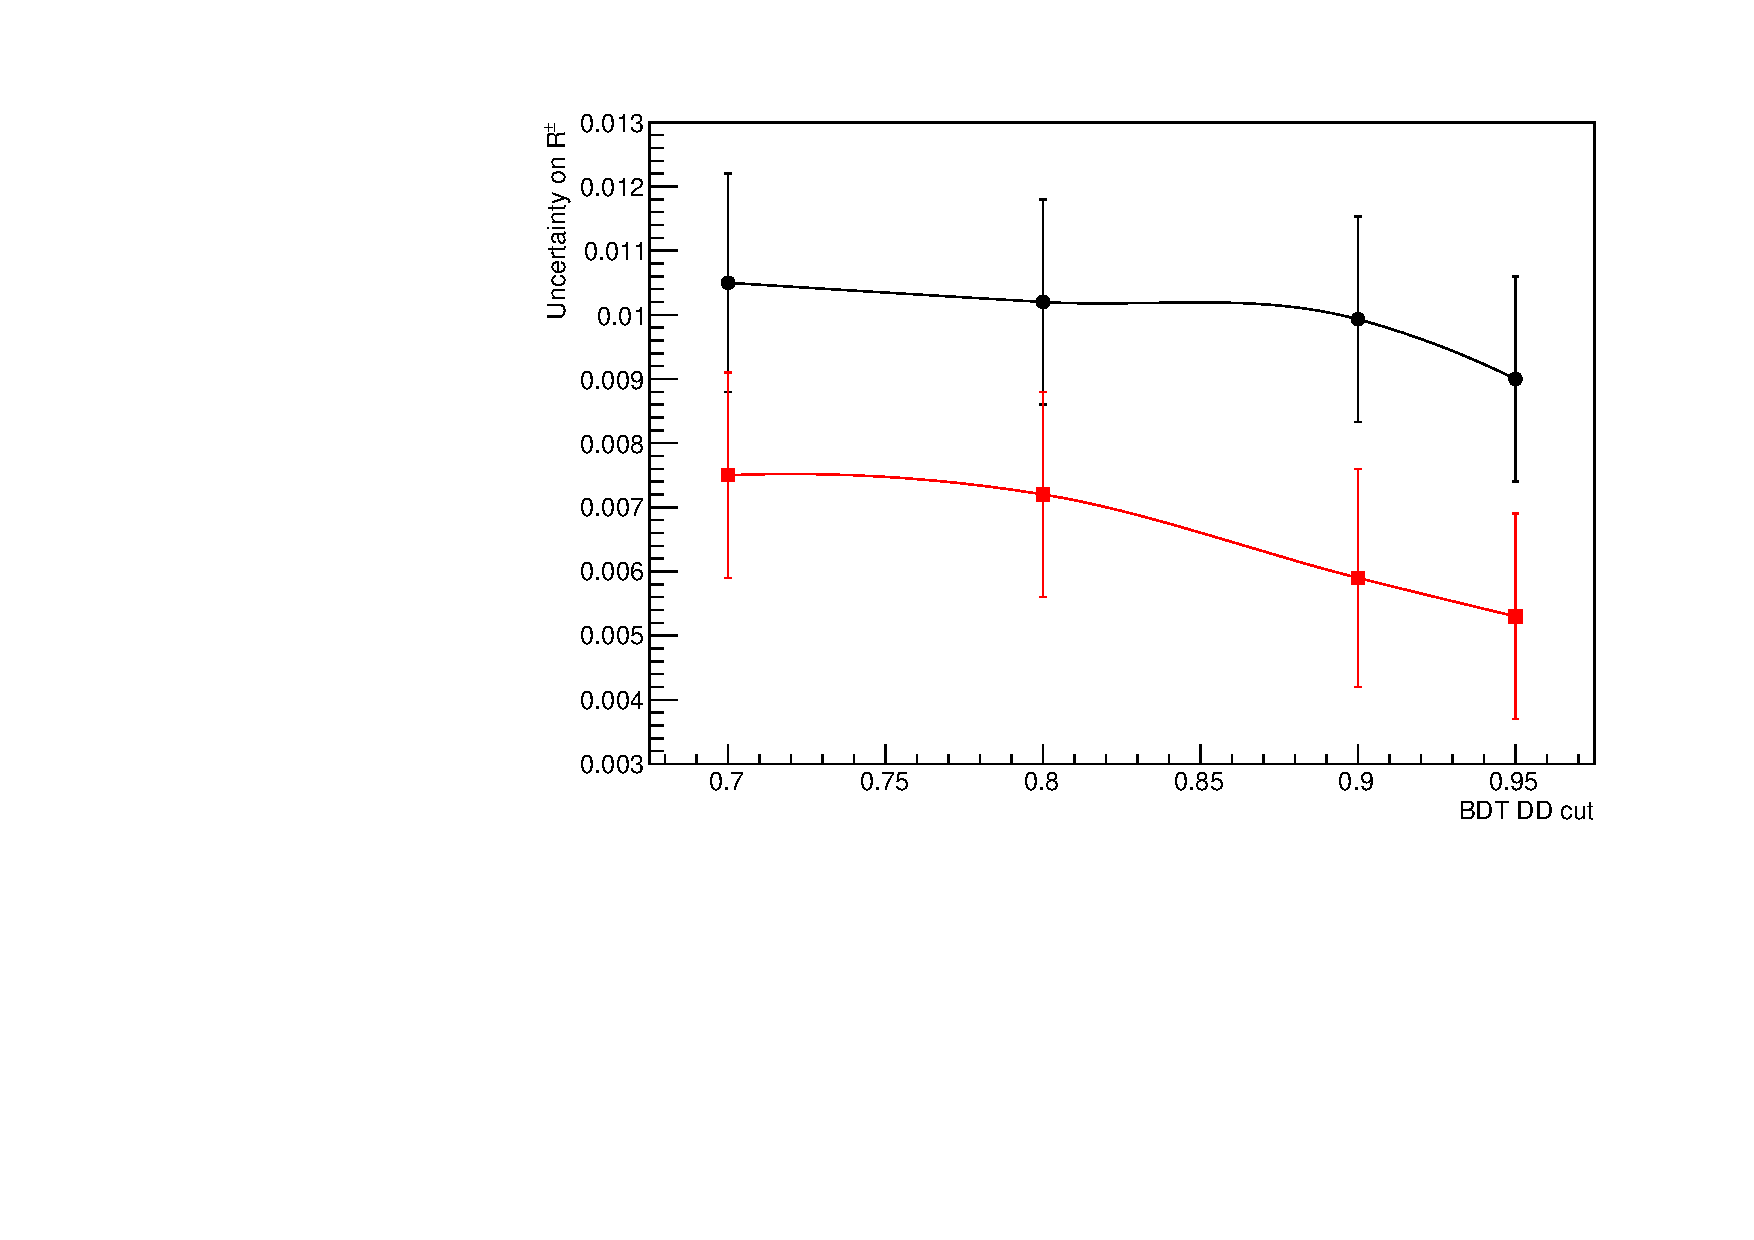
\includegraphics[width=0.8\linewidth]{figures/selection/ADSoptimisation.pdf}
\caption{Value of the uncertainty on $R^+$ and $R^-$ as a function of BDT\_DD cut in the ADS mode. These toys were run with a BDT LL cut of 0.6 on all modes and BDT DD cut of 0.7 on all modes other than the ADS. The black curve is the uncertainty of $R^+$ and the red curve is the uncertainty of $R^-$. Although the uncertainty continues to decrease for a BDT cut of 0.95, this resulted in a significant drop in signal efficiency, therefore a cut of 0.9 was chosen for the ADS}
\label{adsoptimisation}
\end{figure}

The final selection chosen was:

\begin{itemize}
\item{75 MeV \Kstar mass window}
\item{\textbar cos(\KS helicity angle) \textbar $>$ 0.3}
\item{BDT $>$ 0.6 for LL and 0.7 for DD, except in the ADS mode where BDT $>$ 0.6 for LL and 0.9 for DD}
\end{itemize}

The choice of BDT selection in ADS mode remains optimal when tested against a scenario of low combinatoric in the ADS mode. 

%%%%%%%%%%%%%%%%%%%%%%%%
\section{Fit results}
\label{sec:cpfit:results}

The fits to data are shown in Figures \ref{datafit2bodyRun1}, \ref{datafit4bodyRun1}, \ref{datafit2bodyRun2} and \ref{datafit4bodyRun2}. Table \ref{cpfitresultsphysics} shows the fit results of the physics parameters of interest and Table \ref{cpfitresultsshapes} shows the fit results for $K\pi$ and $K\pi\pi\pi$ signal yields and shape parameters. All the combinatoric yields are left floating in the fit and these results are tabulated in Appendix \ref{sec:app:cpfit}.

The fitted yields obtained for running the fit with \Bp and \Bm samples combined are given in Table \ref{fittedyields}. 

\begin{sidewaysfigure}[h]
\centering
\subfloat[$K\pi$, LL]{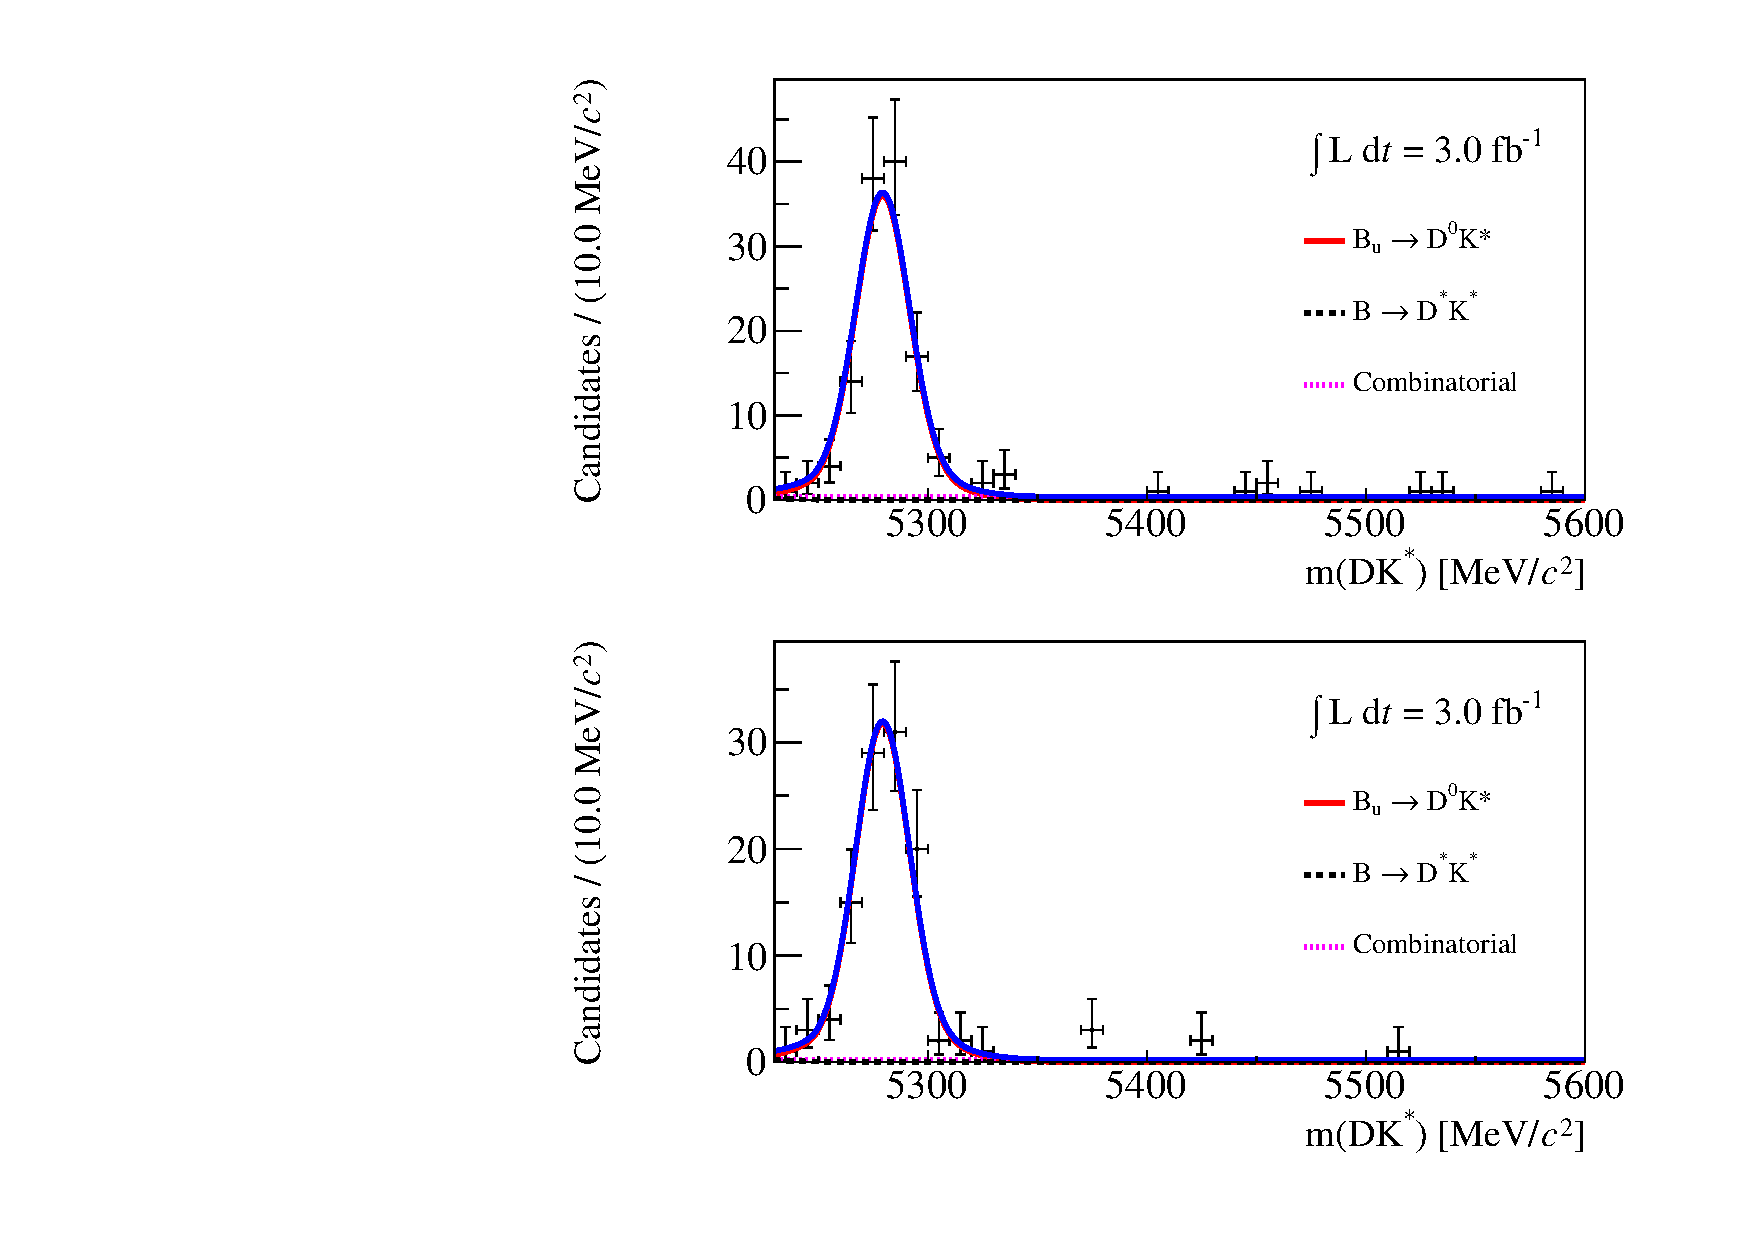
\includegraphics[width=0.25\linewidth]{figures/results/canvas_d2kpi_LL_run1.pdf}}
\hfill
\subfloat[$KK$, LL]{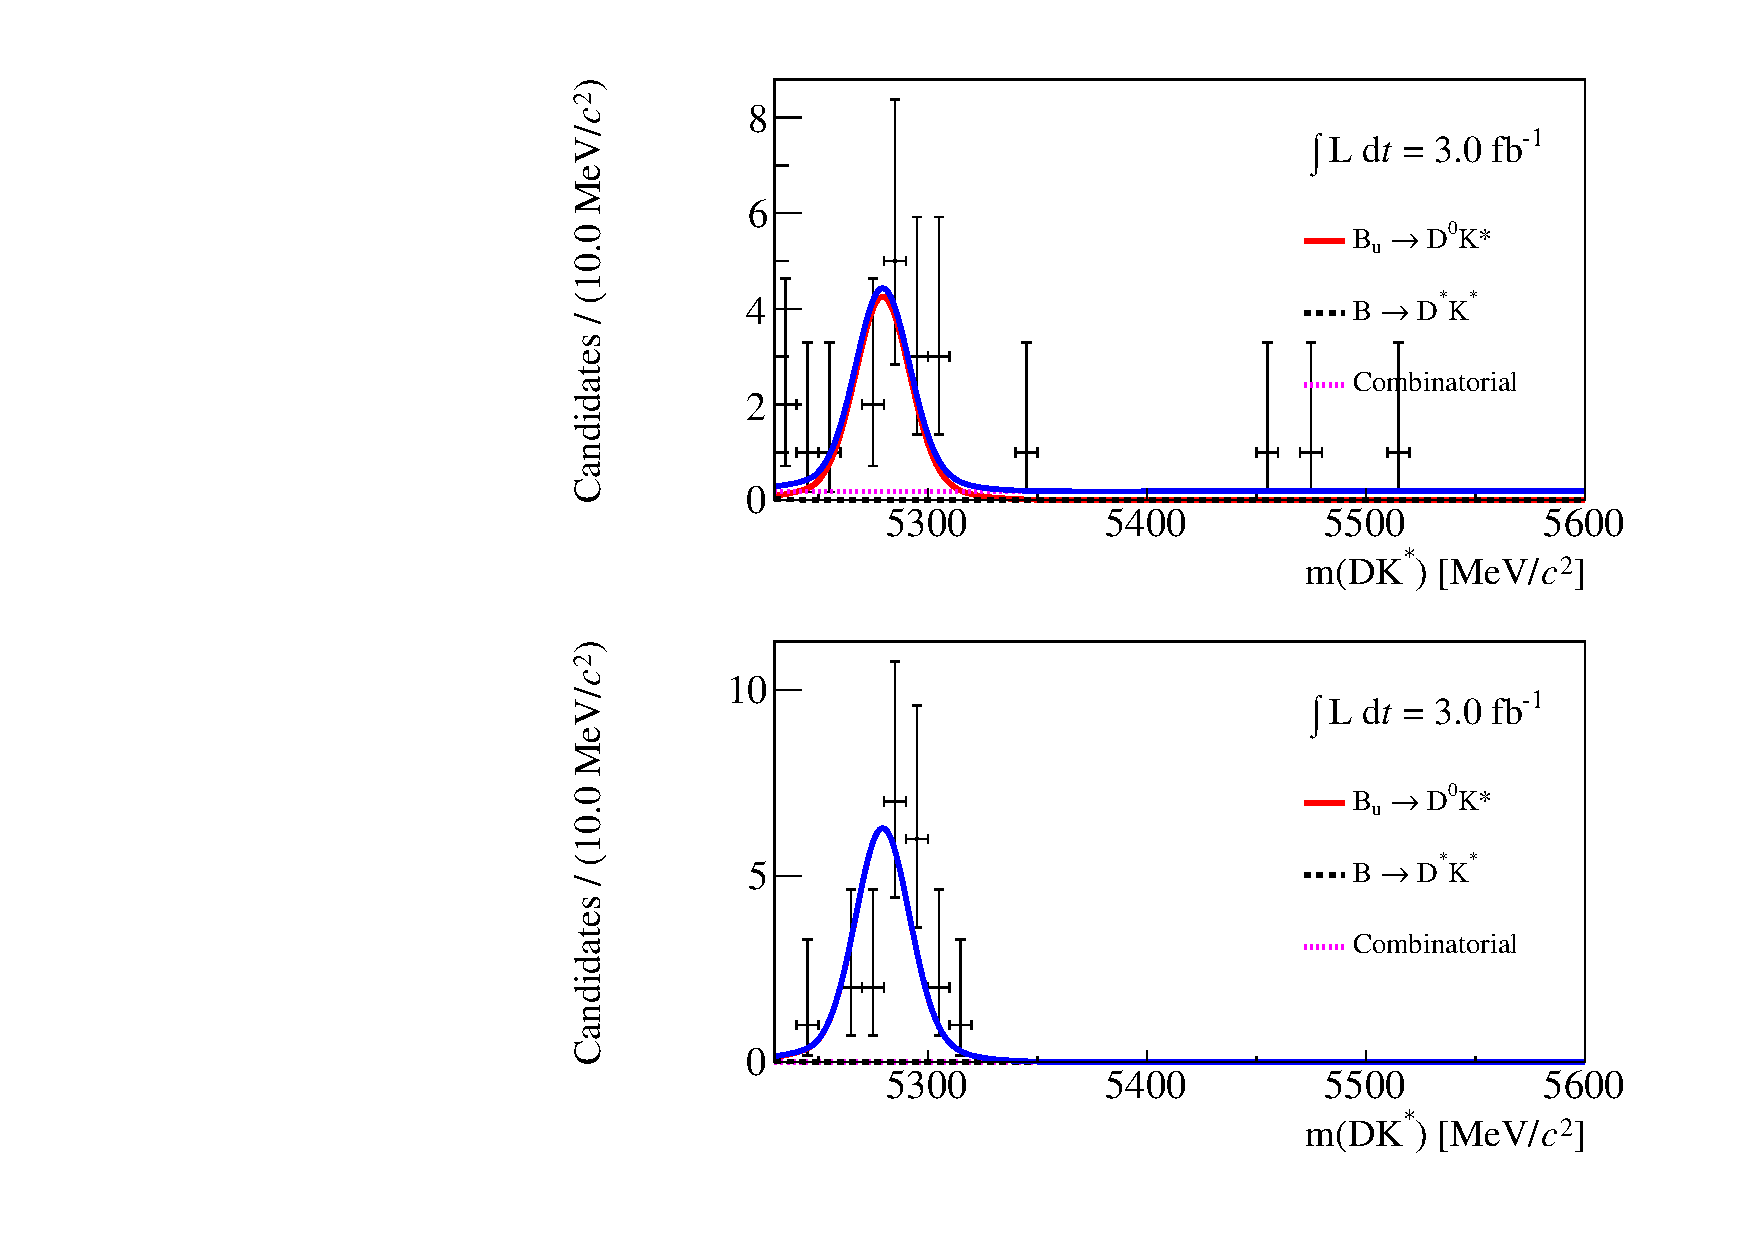
\includegraphics[width=0.25\linewidth]{figures/results/canvas_d2kk_LL_run1.pdf}}
\hfill
\subfloat[$\pi\pi$, LL]{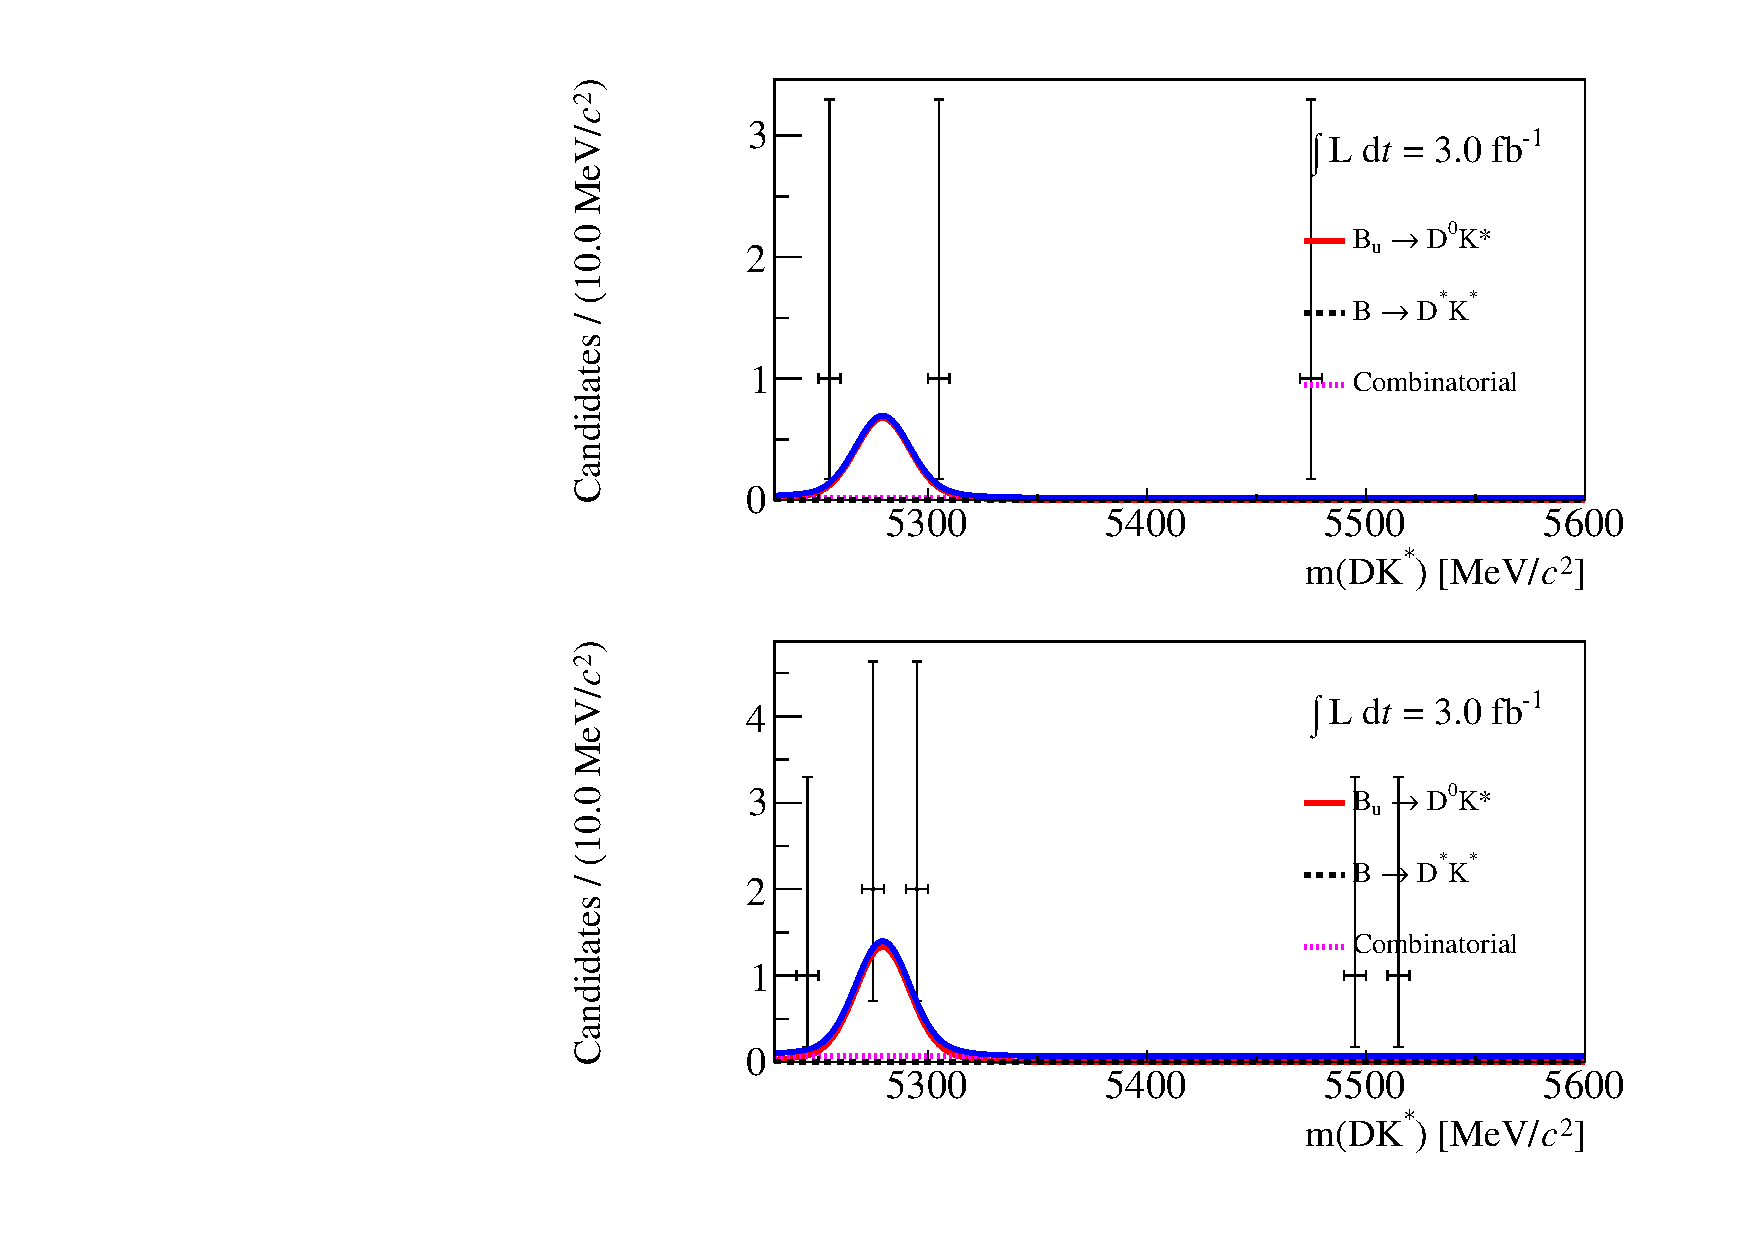
\includegraphics[width=0.25\linewidth]{figures/results/canvas_d2pipi_LL_run1.pdf}}
\hfill
\subfloat[$\pi K$, LL]{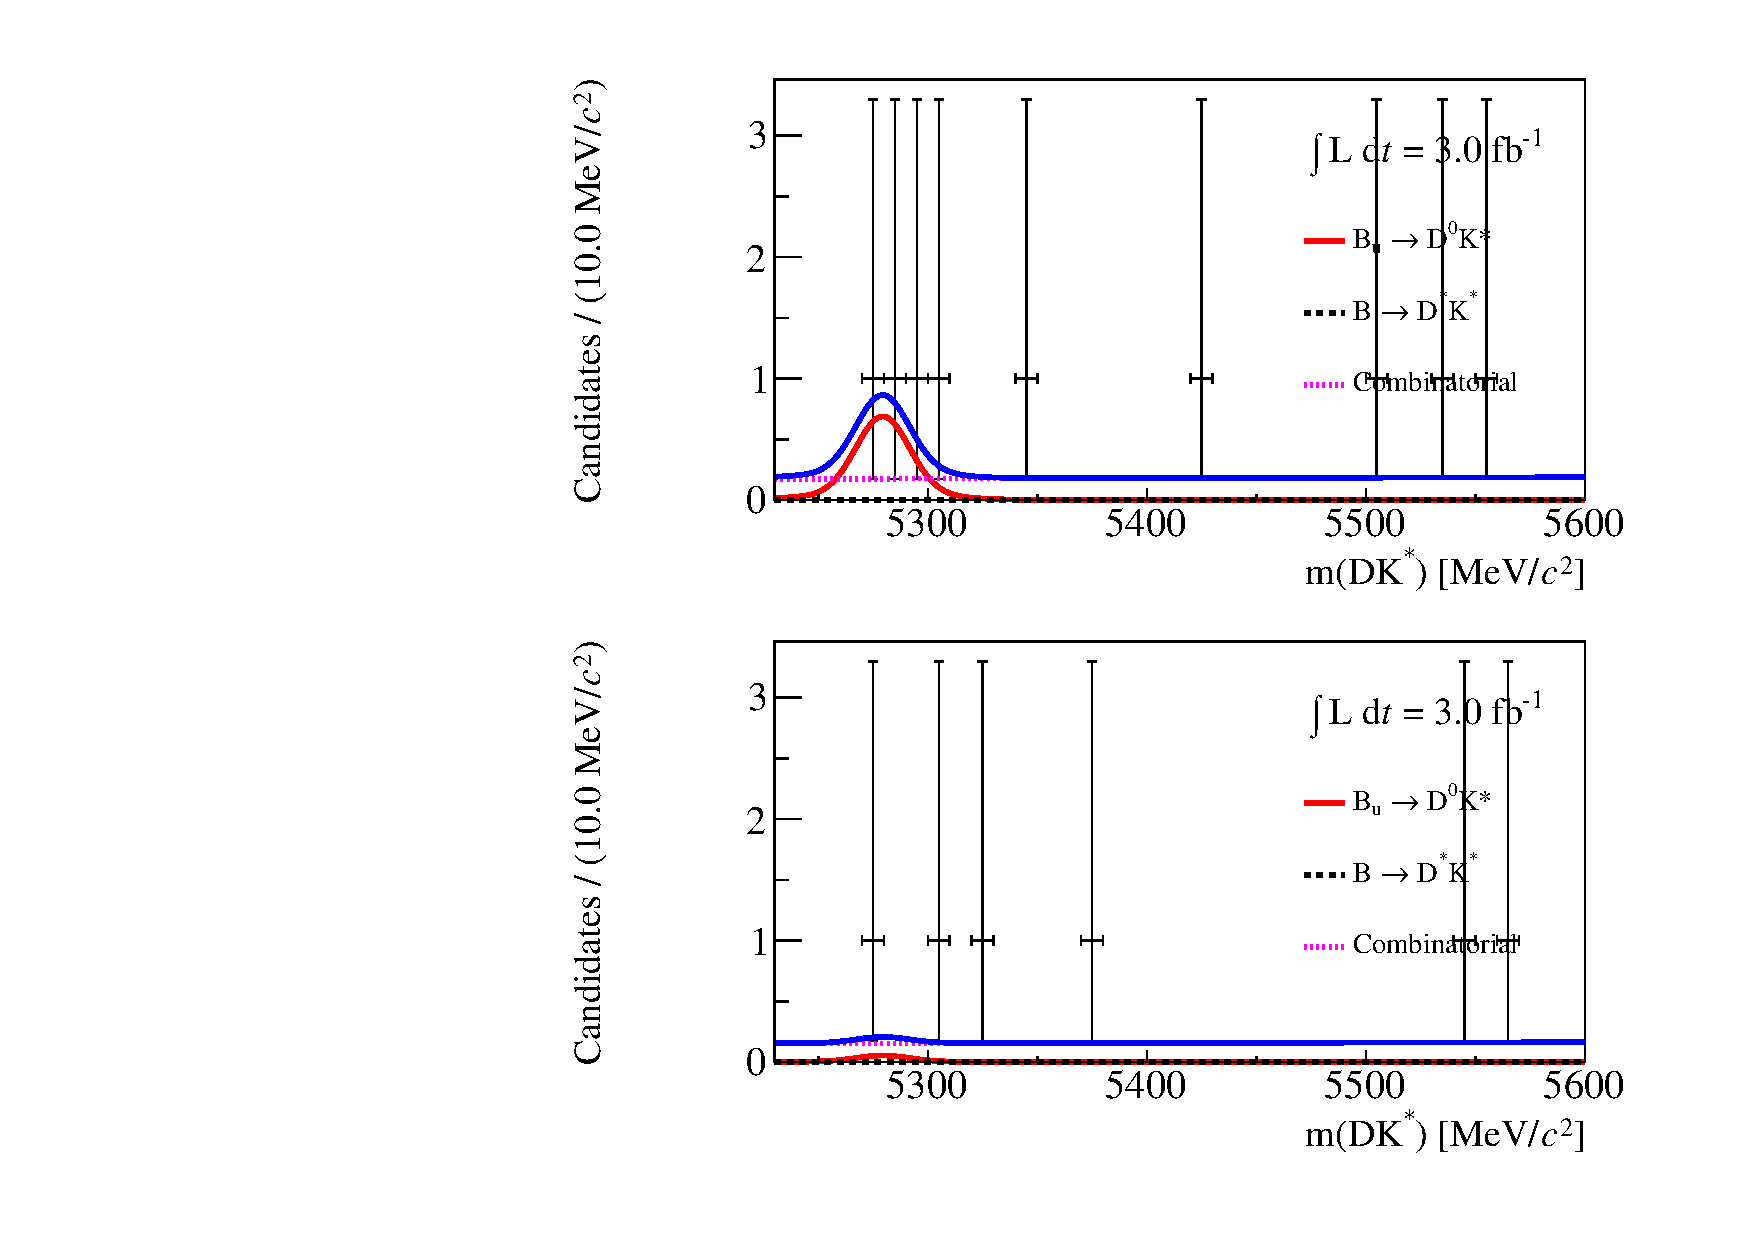
\includegraphics[width=0.25\linewidth]{figures/results/canvas_d2pik_LL_run1.pdf}}
\hfill
\subfloat[$K\pi$, DD]{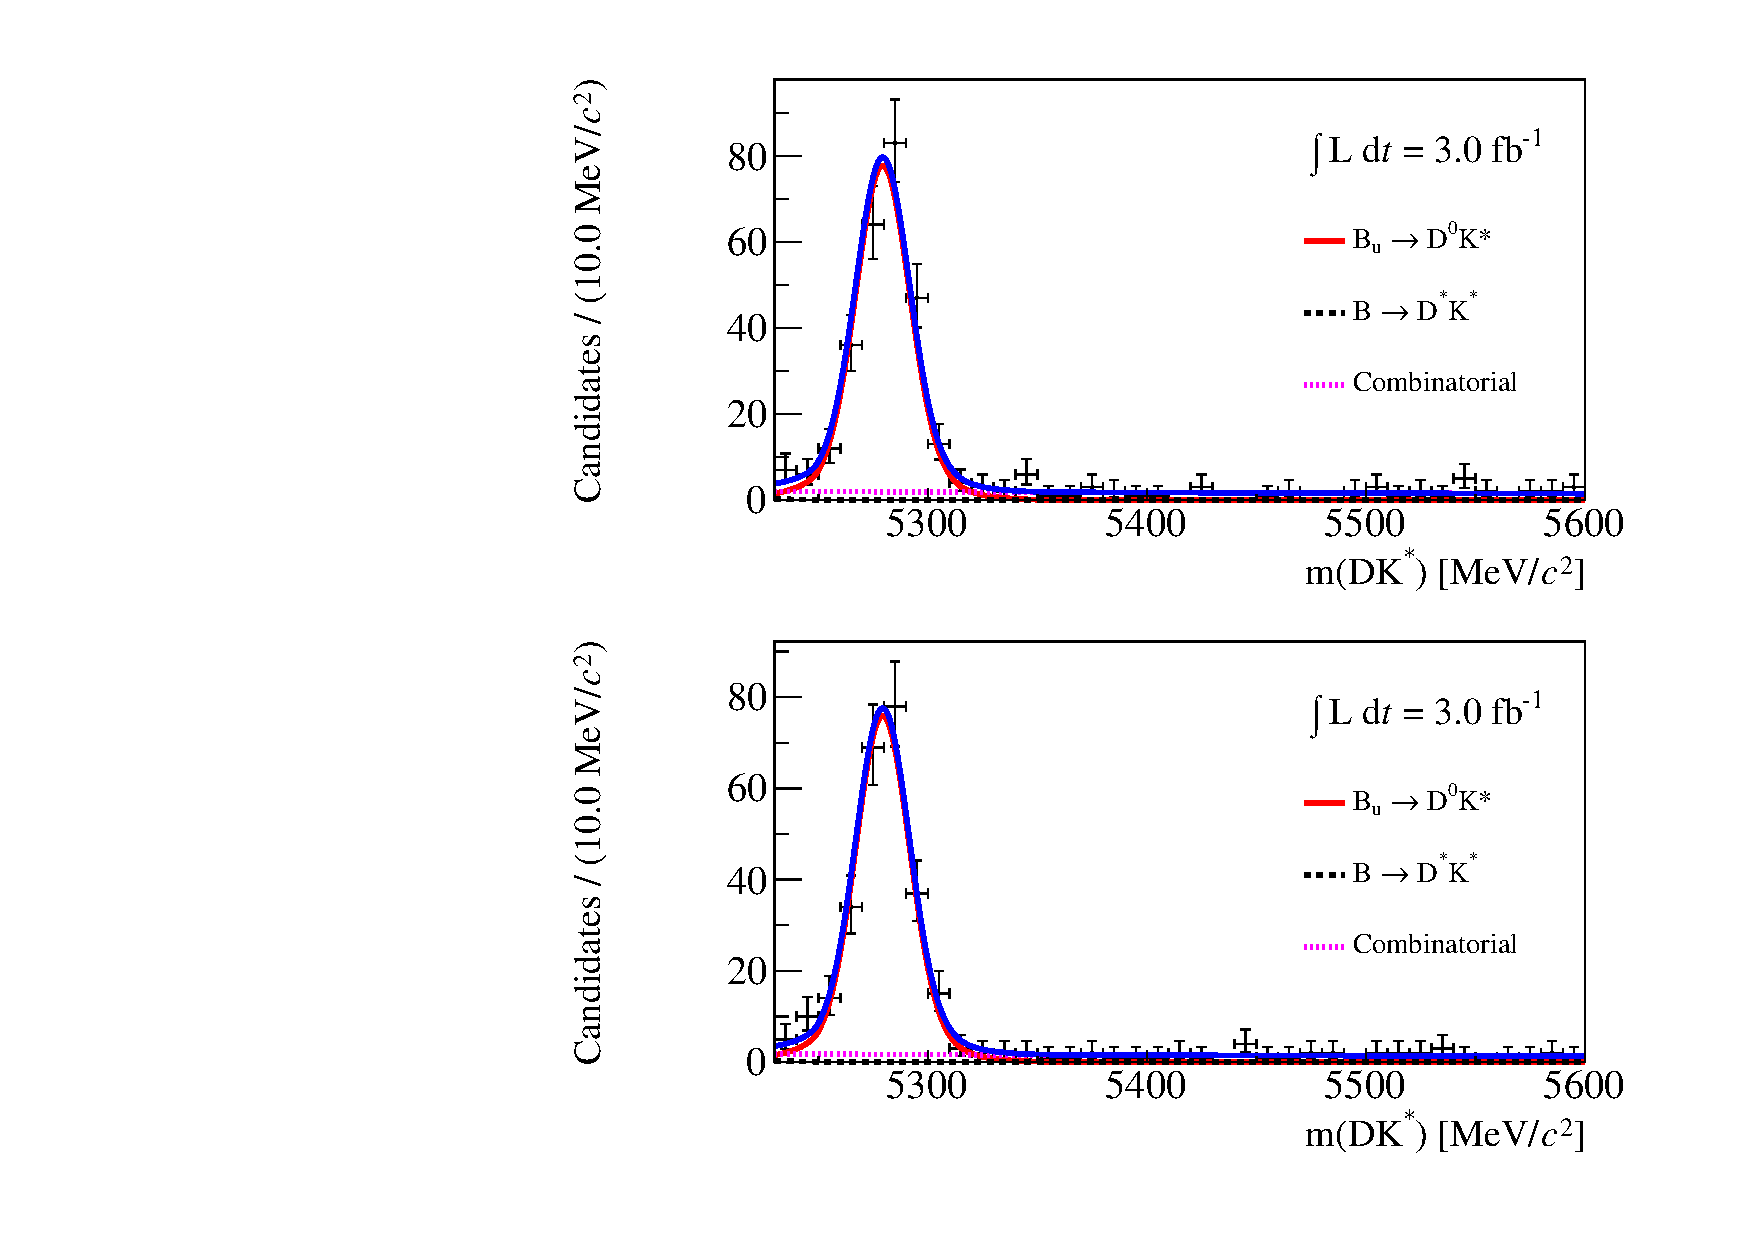
\includegraphics[width=0.25\linewidth]{figures/results/canvas_d2kpi_DD_run1.pdf}}
\hfill
\subfloat[$KK$, DD]{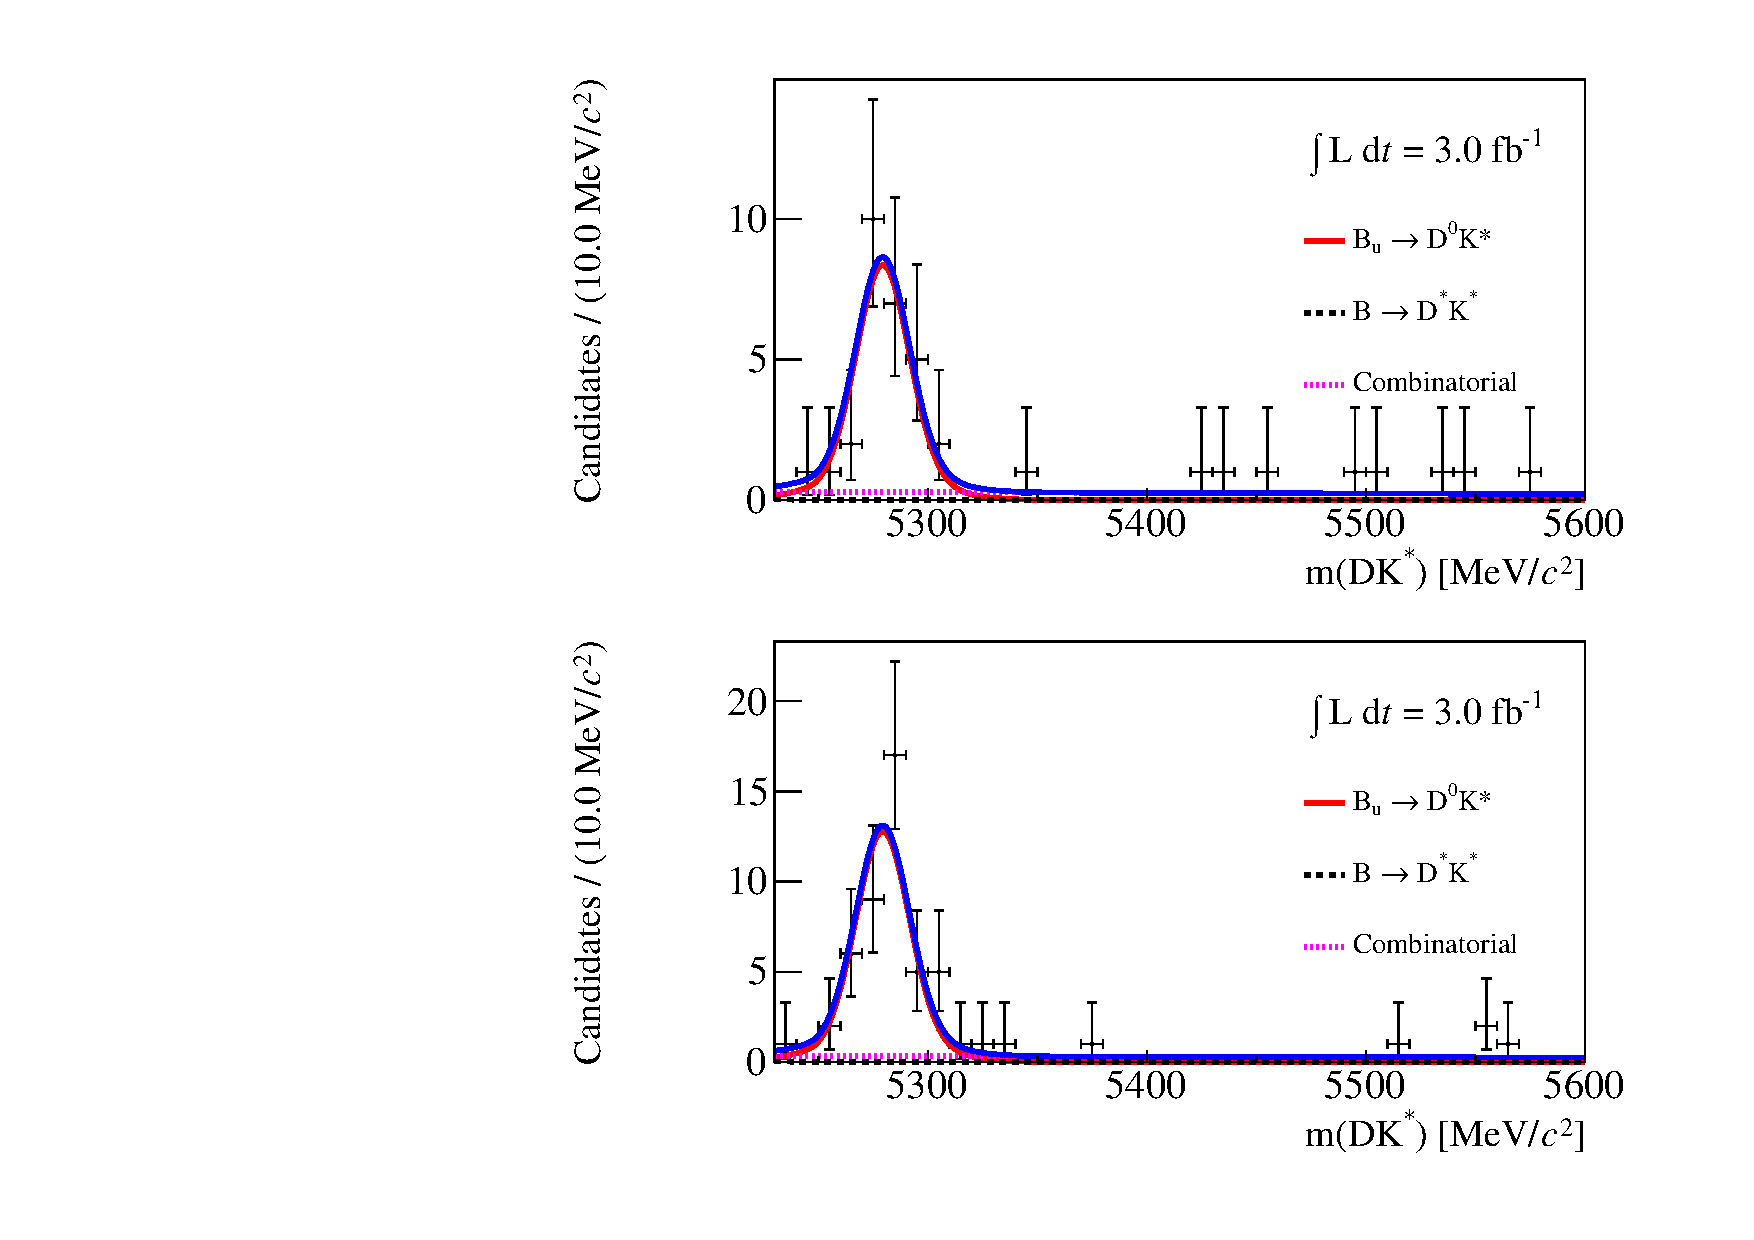
\includegraphics[width=0.25\linewidth]{figures/results/canvas_d2kk_DD_run1.pdf}}
\hfill
\subfloat[$\pi\pi$, DD]{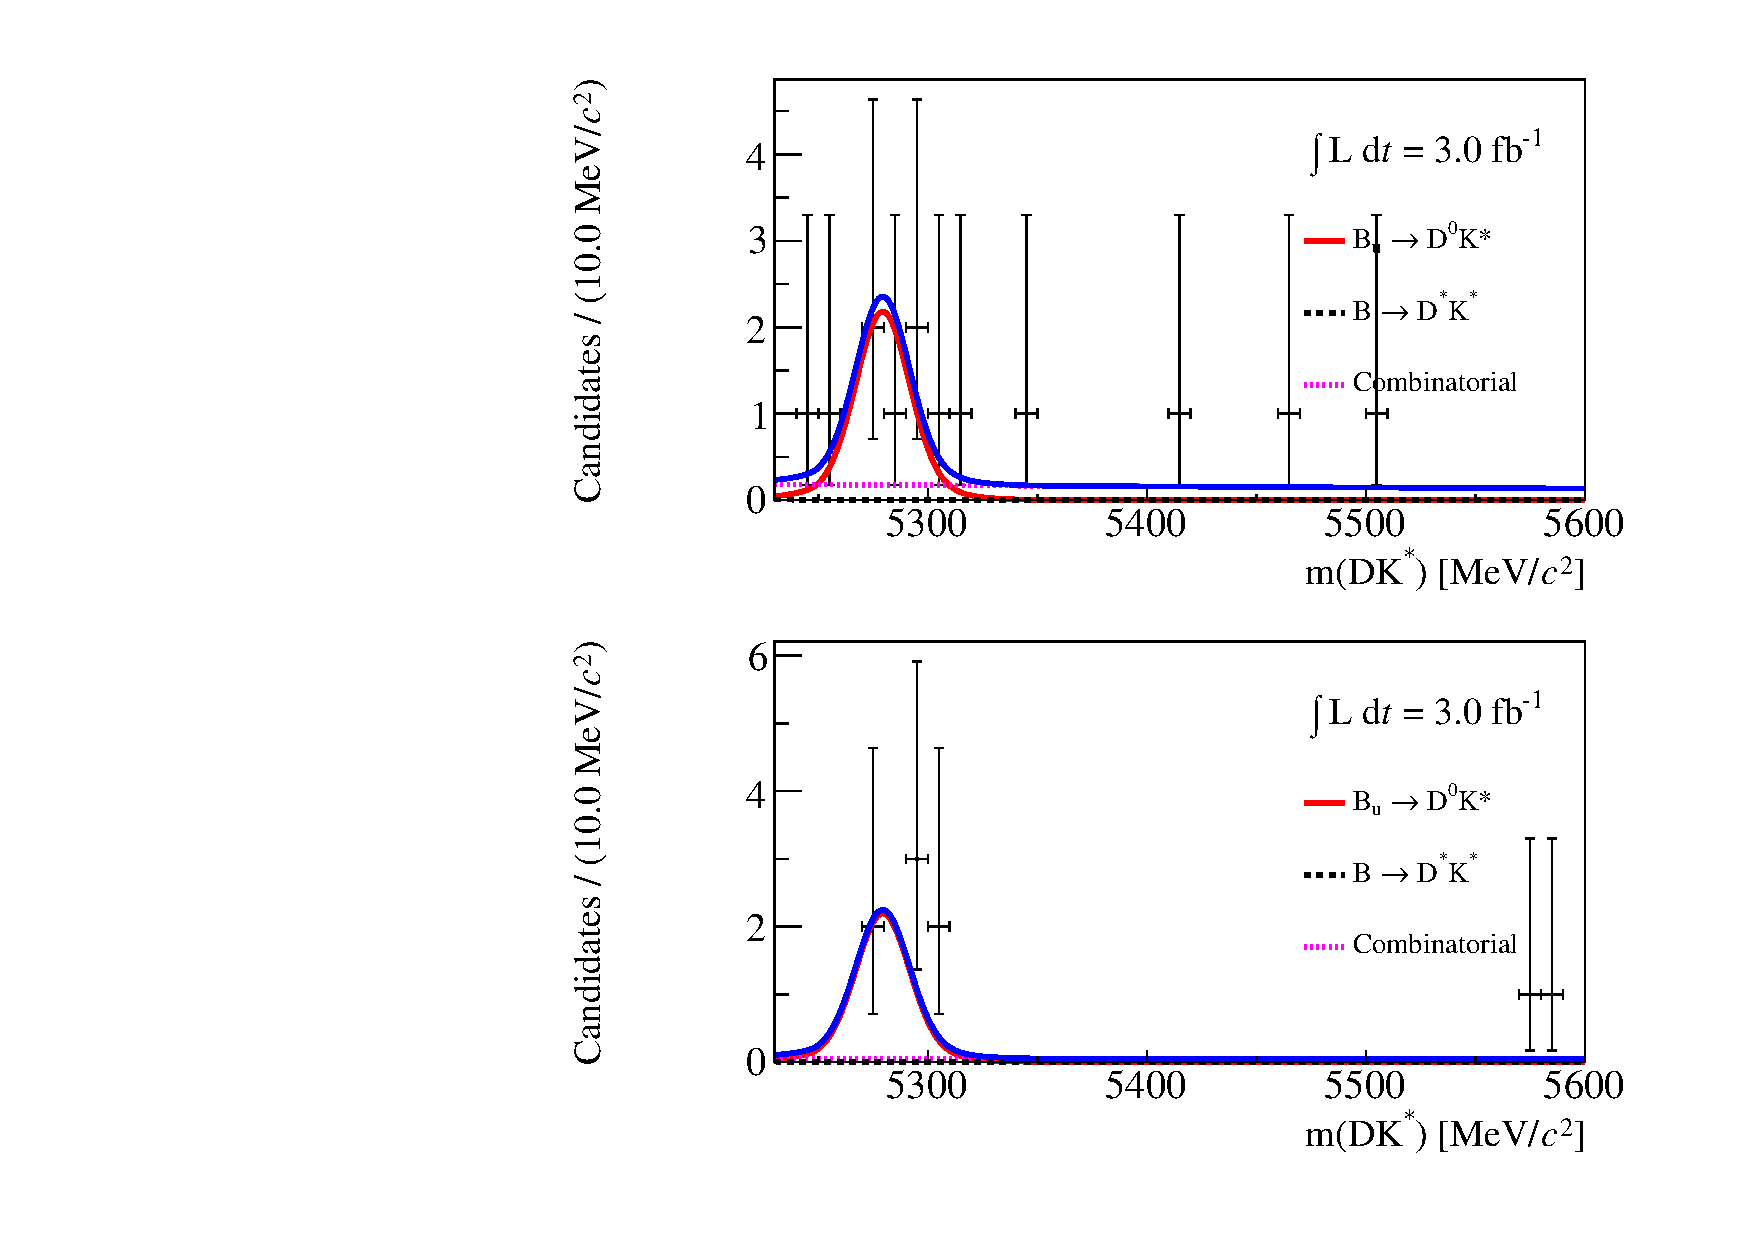
\includegraphics[width=0.25\linewidth]{figures/results/canvas_d2pipi_DD_run1.pdf}}
\hfill
\subfloat[$\pi K$, DD]{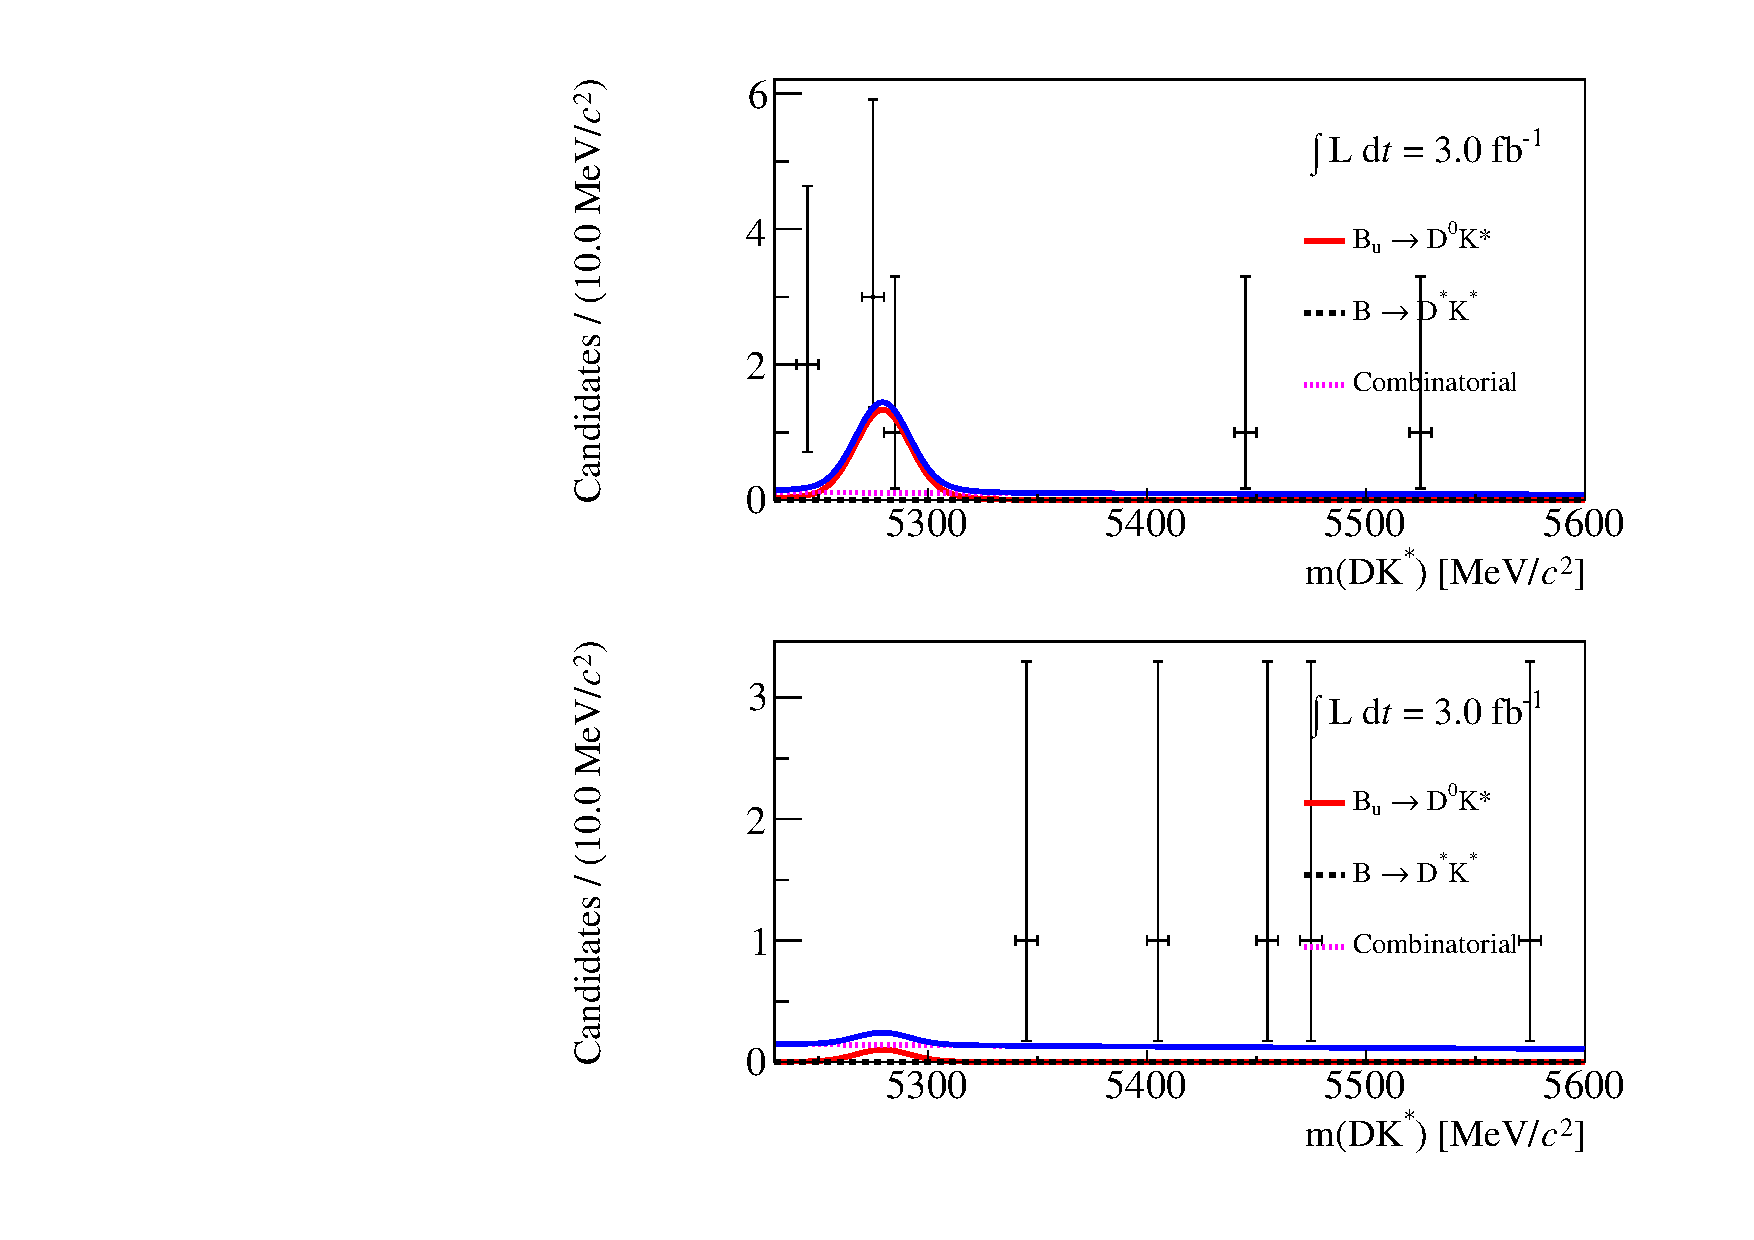
\includegraphics[width=0.25\linewidth]{figures/results/canvas_d2pik_DD_run1.pdf}}
\caption{Results of the simultaneous fit for Run 1 data for 2-body modes. In each pair the top plot is for \Bp decays and the bottom plot is for \Bm decays.}
\label{datafit2bodyRun1}
\end{sidewaysfigure}

\begin{sidewaysfigure}[h]
\centering
\subfloat[$K\pi\pi\pi$, LL]{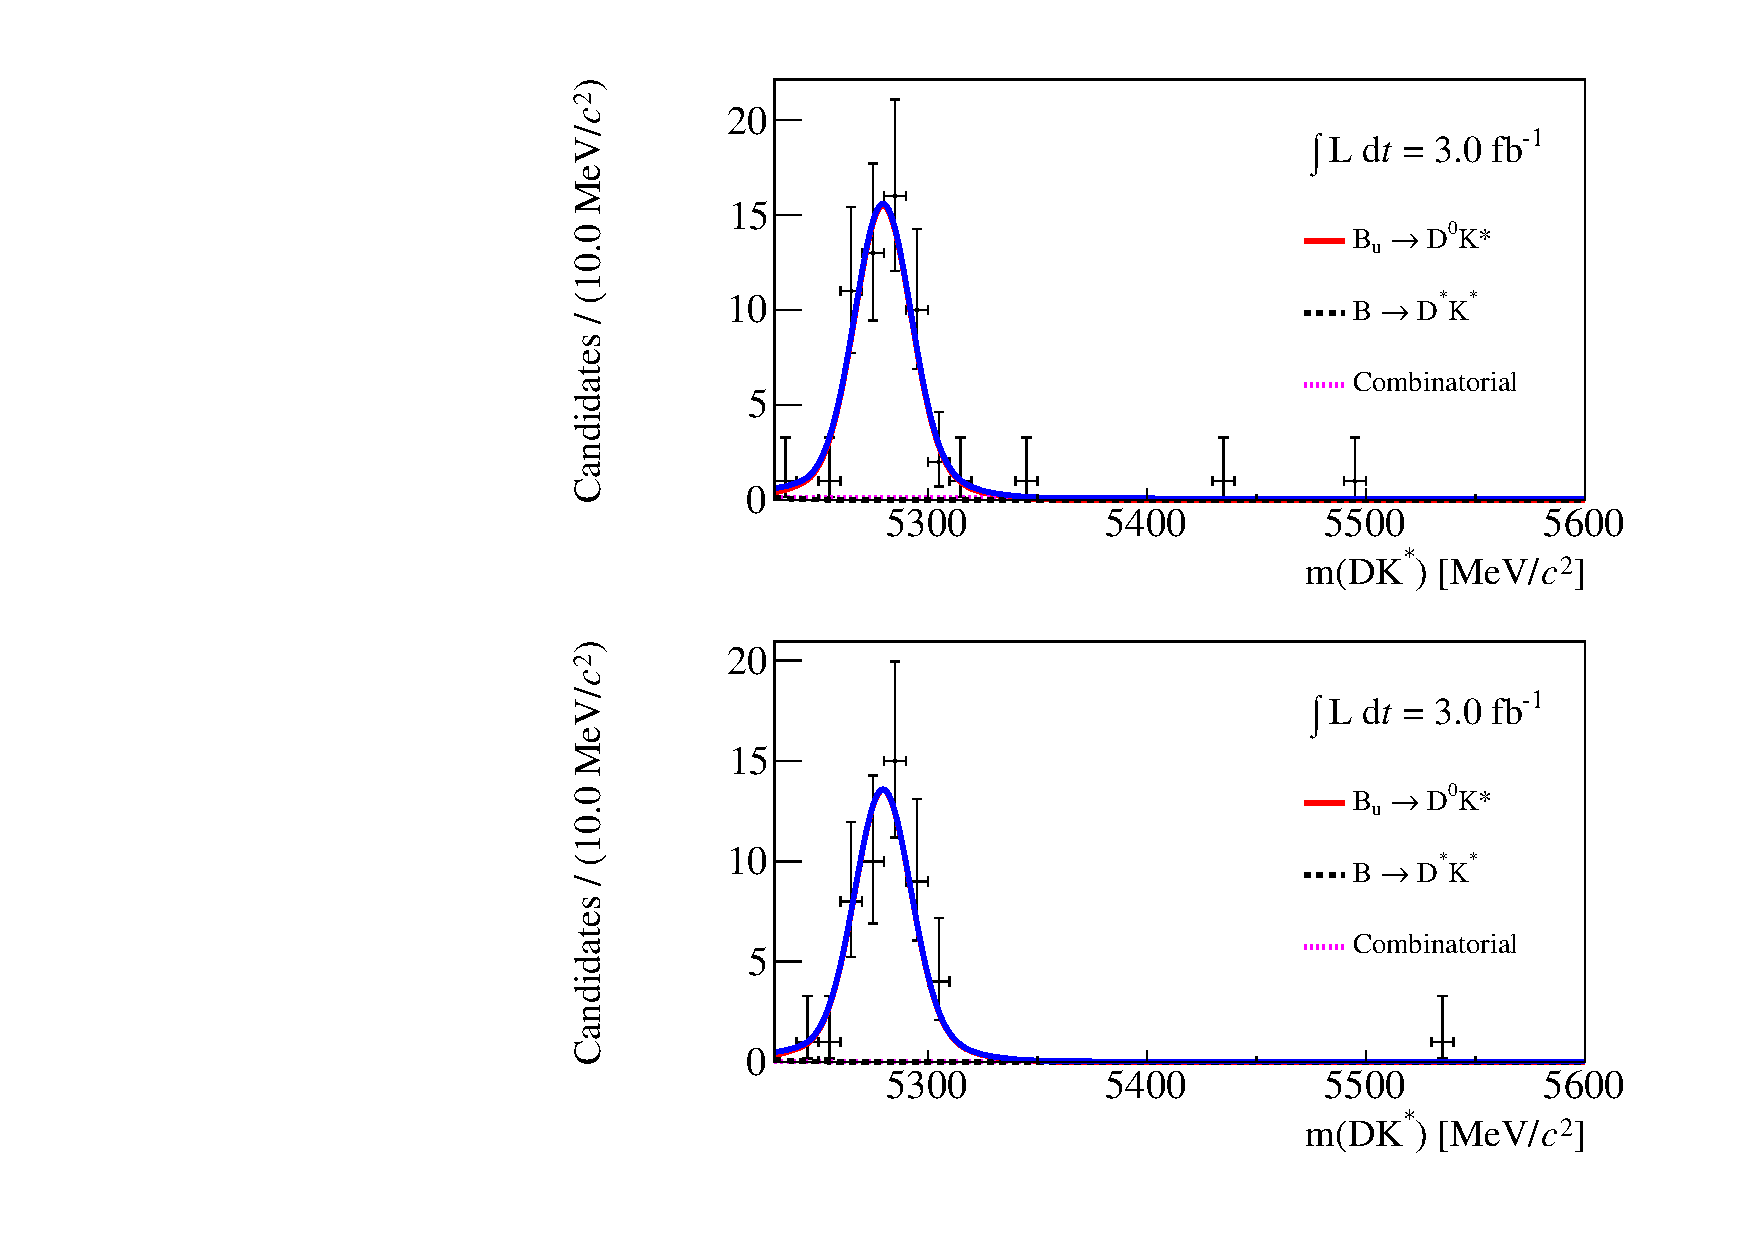
\includegraphics[width=0.3\linewidth]{figures/results/canvas_d2kpipipi_LL_run1.pdf}}
\hfill
\subfloat[$\pi\pi\pi\pi$, LL]{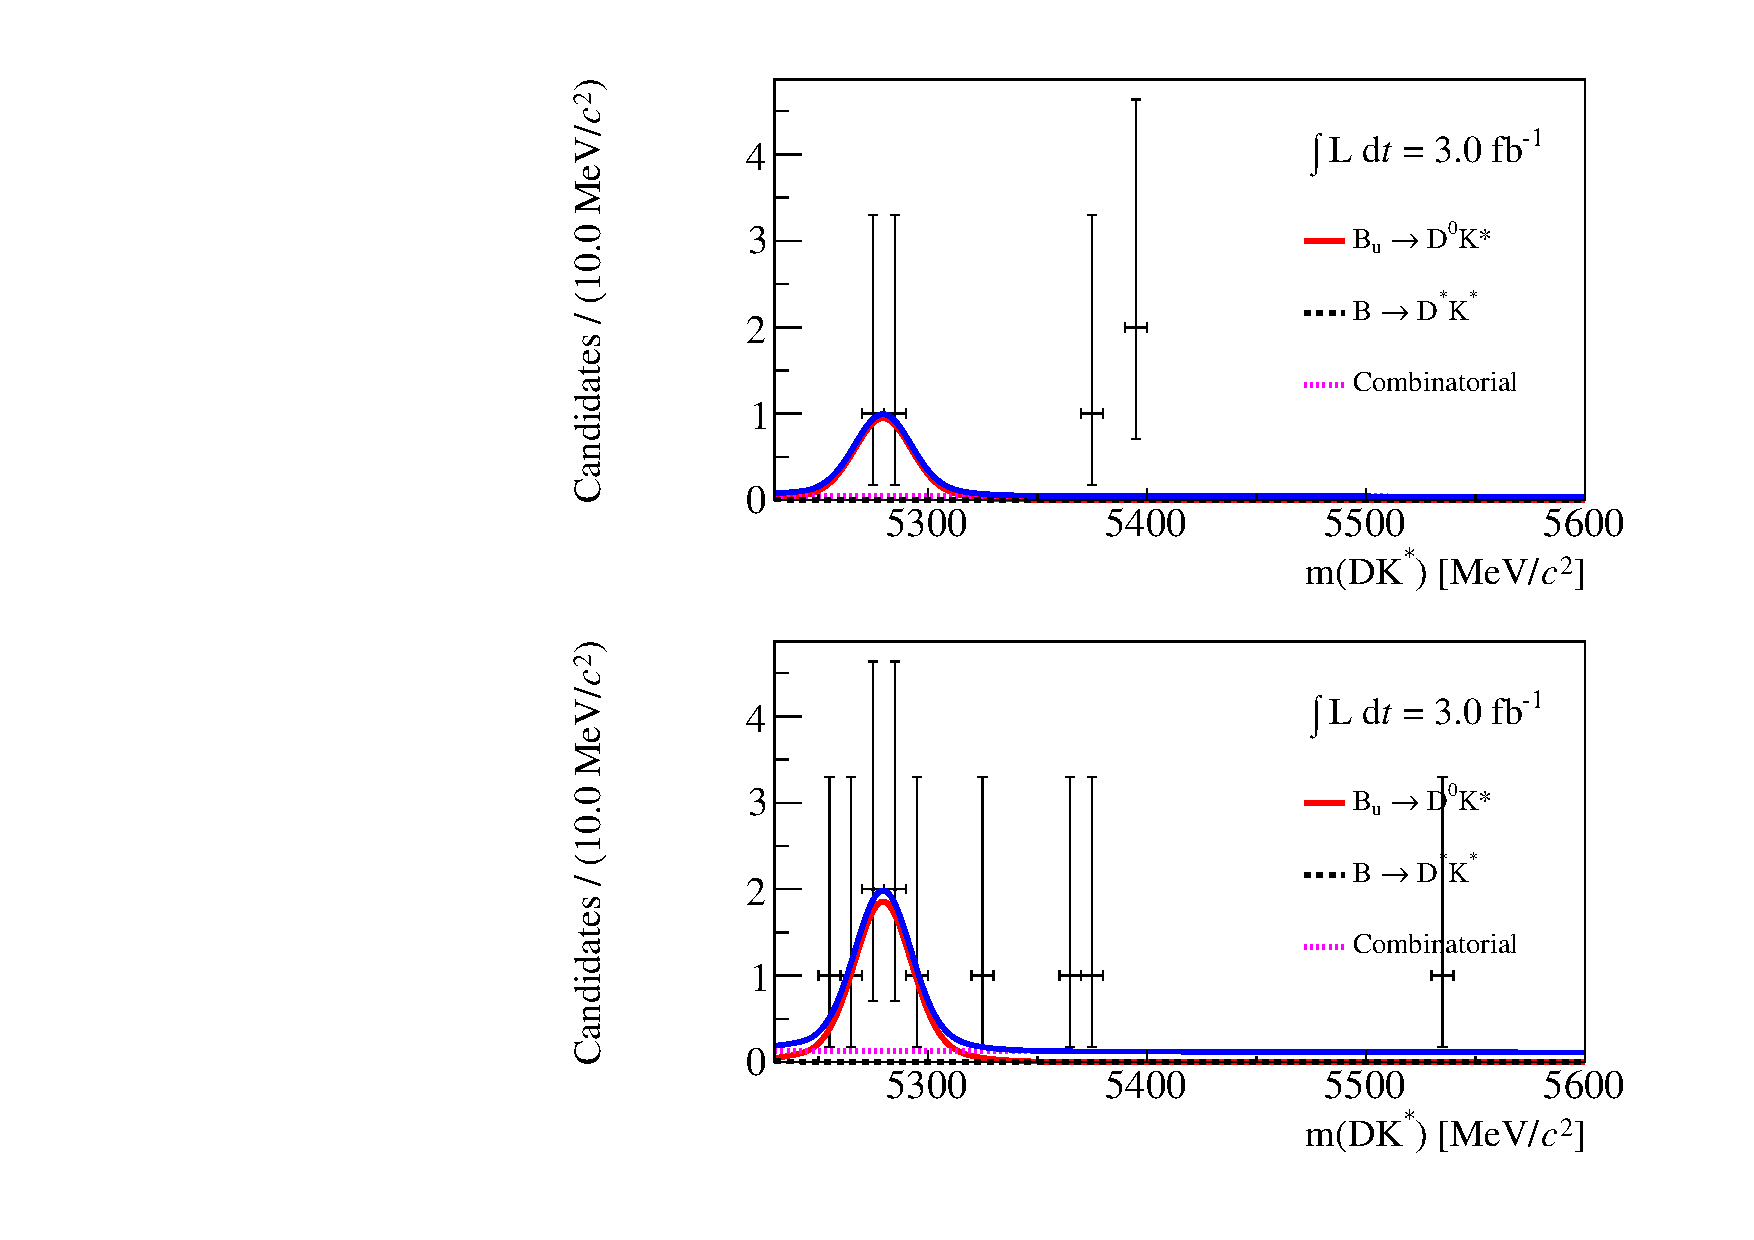
\includegraphics[width=0.3\linewidth]{figures/results/canvas_d2pipipipi_LL_run1.pdf}}
\hfill
\subfloat[$\pi K\pi\pi$, LL]{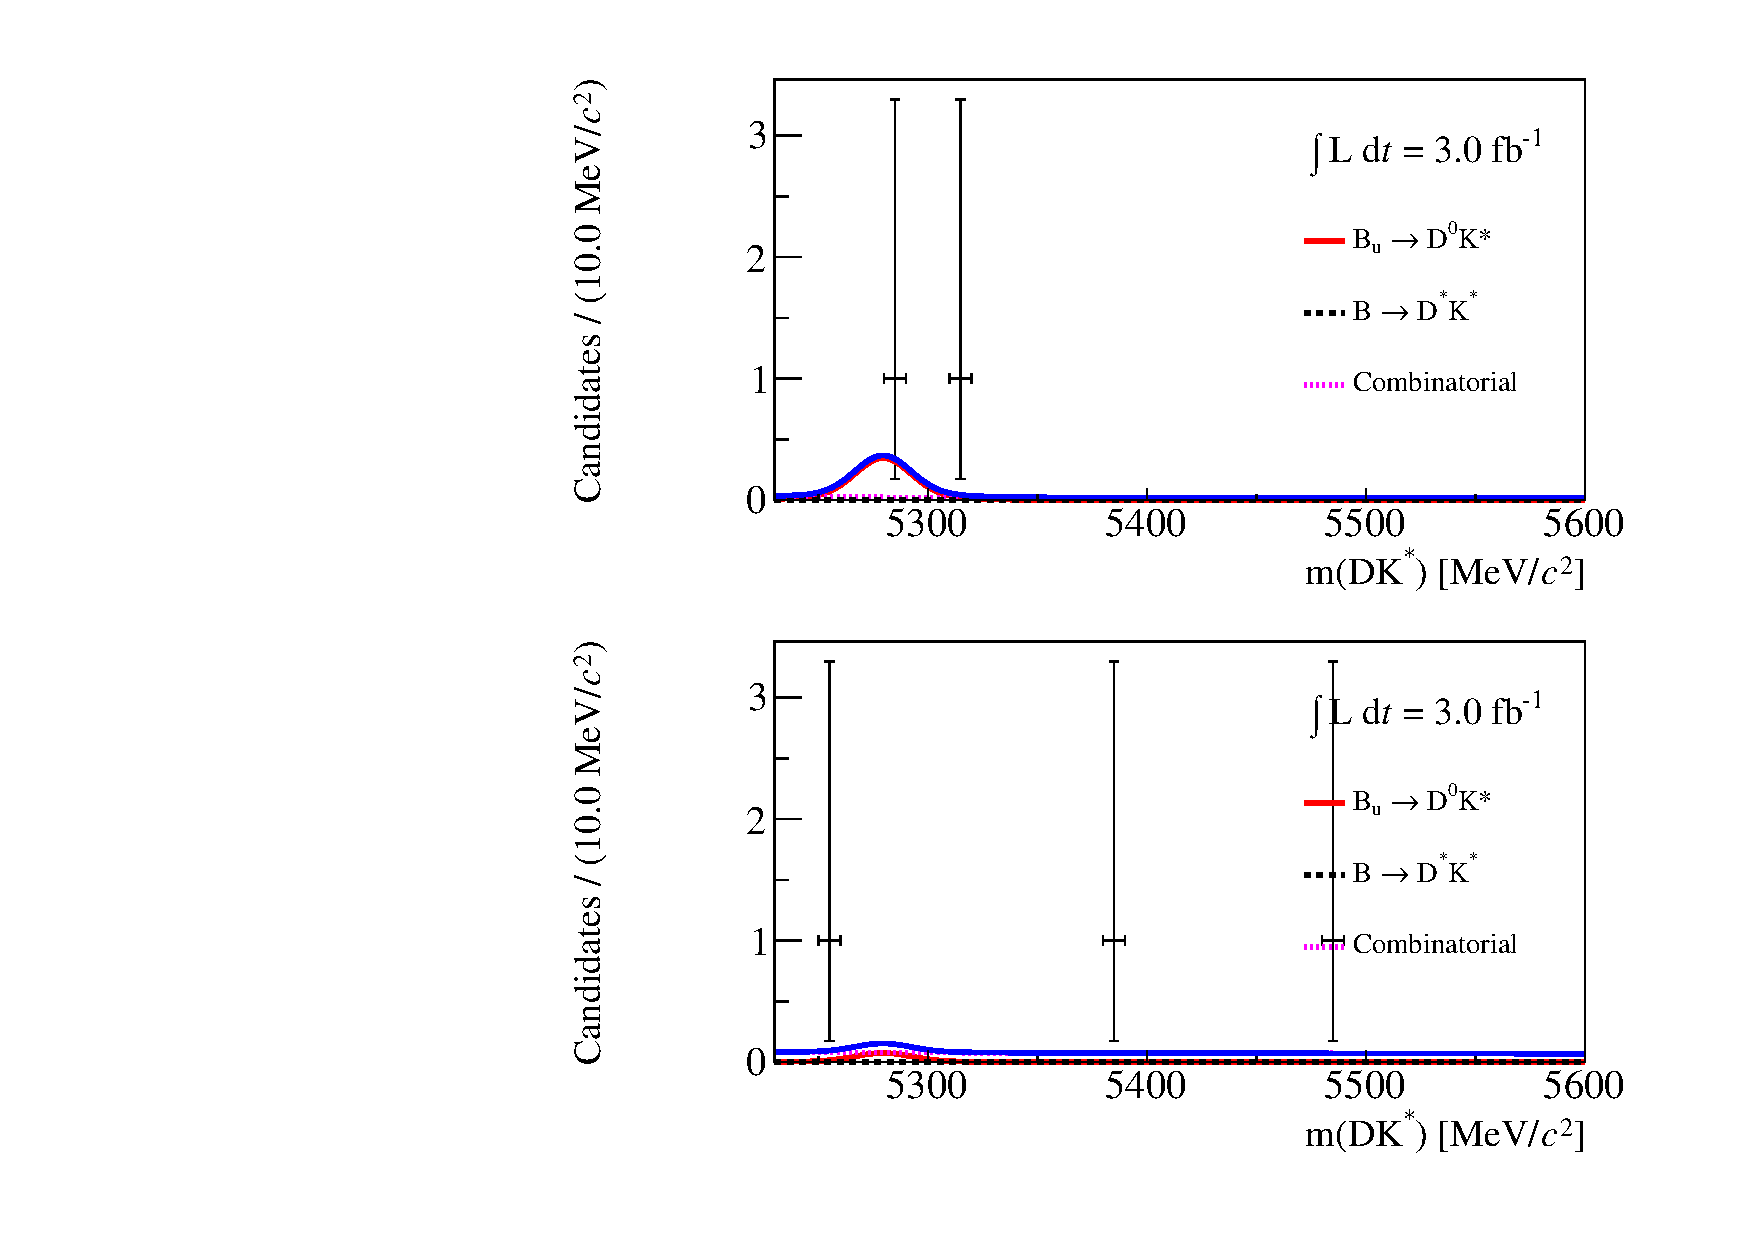
\includegraphics[width=0.3\linewidth]{figures/results/canvas_d2pikpipi_LL_run1.pdf}}
\hfill
\subfloat[$K\pi\pi\pi$, DD]{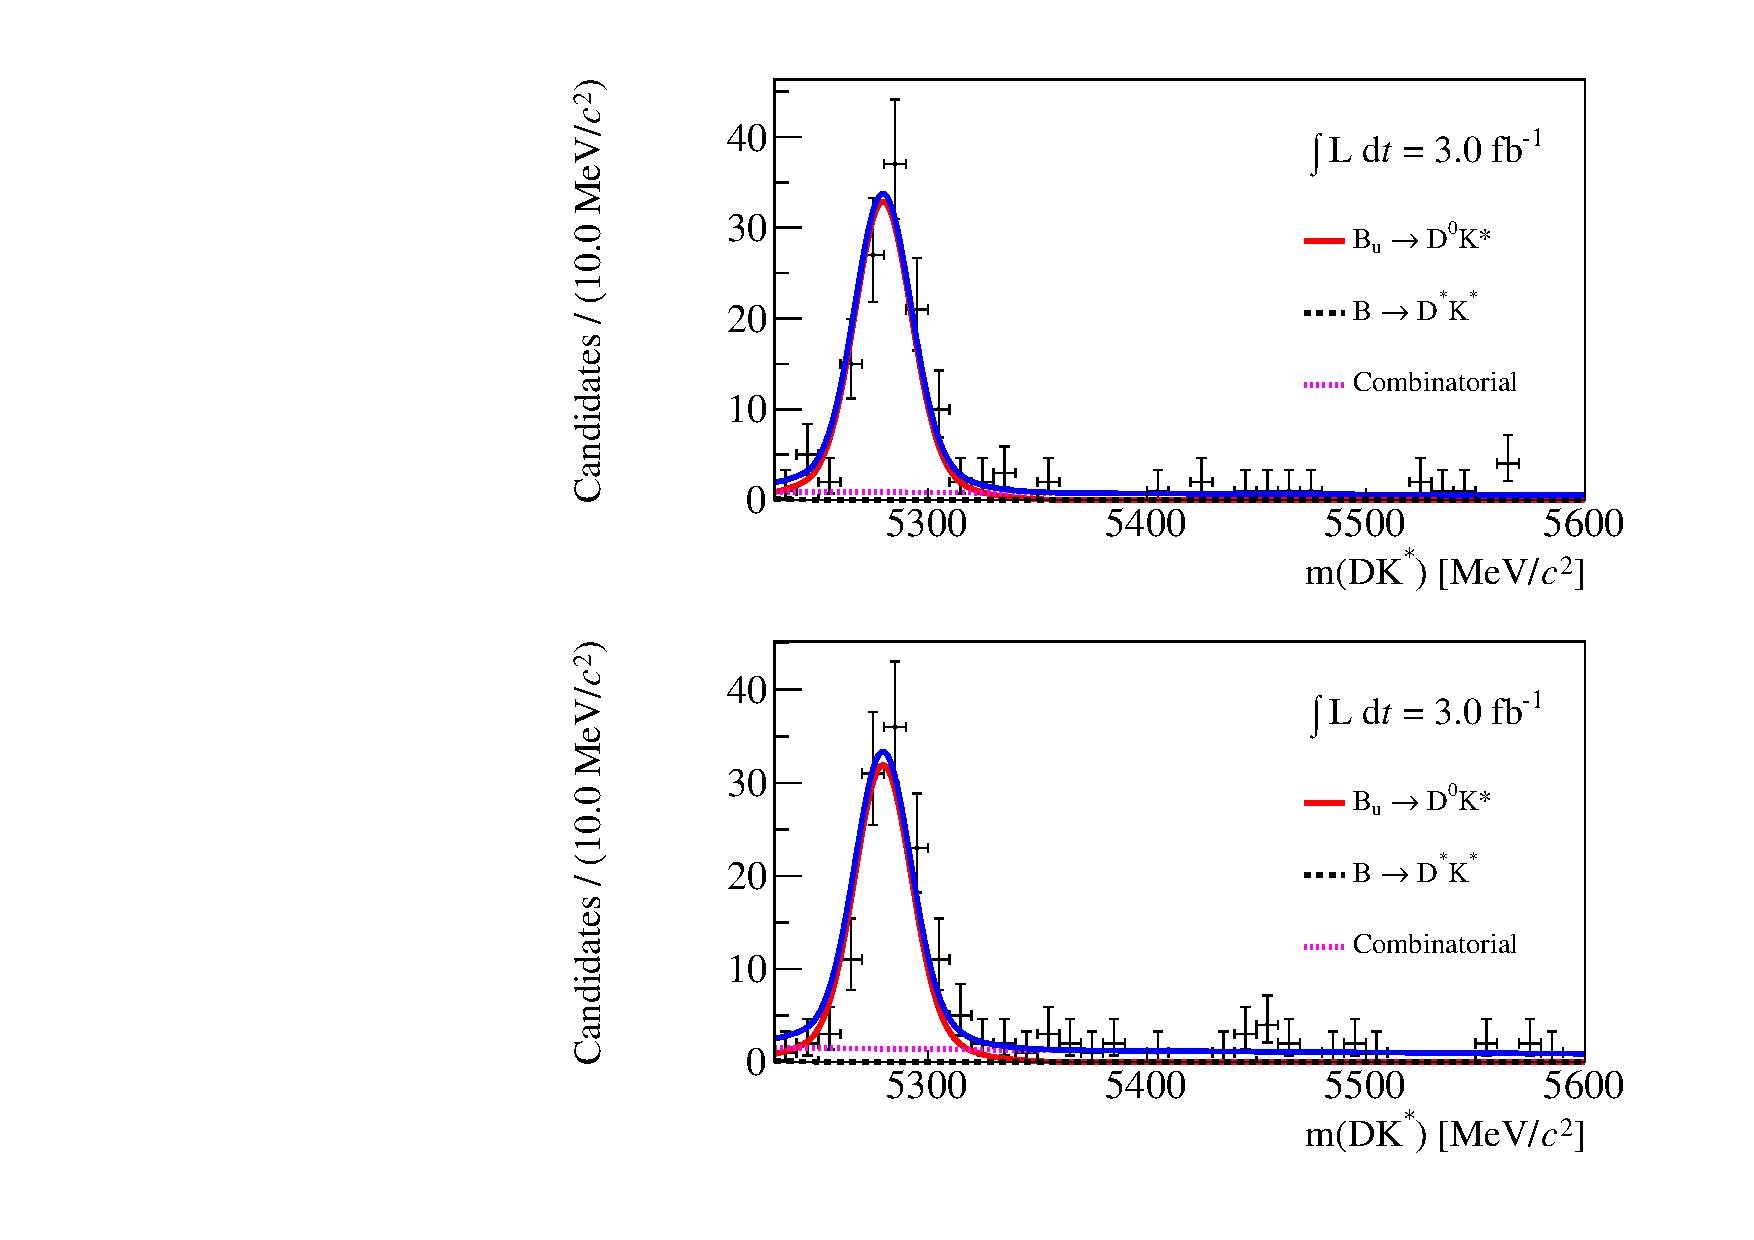
\includegraphics[width=0.3\linewidth]{figures/results/canvas_d2kpipipi_DD_run1.pdf}}
\hfill
\subfloat[$\pi\pi\pi\pi$, DD]{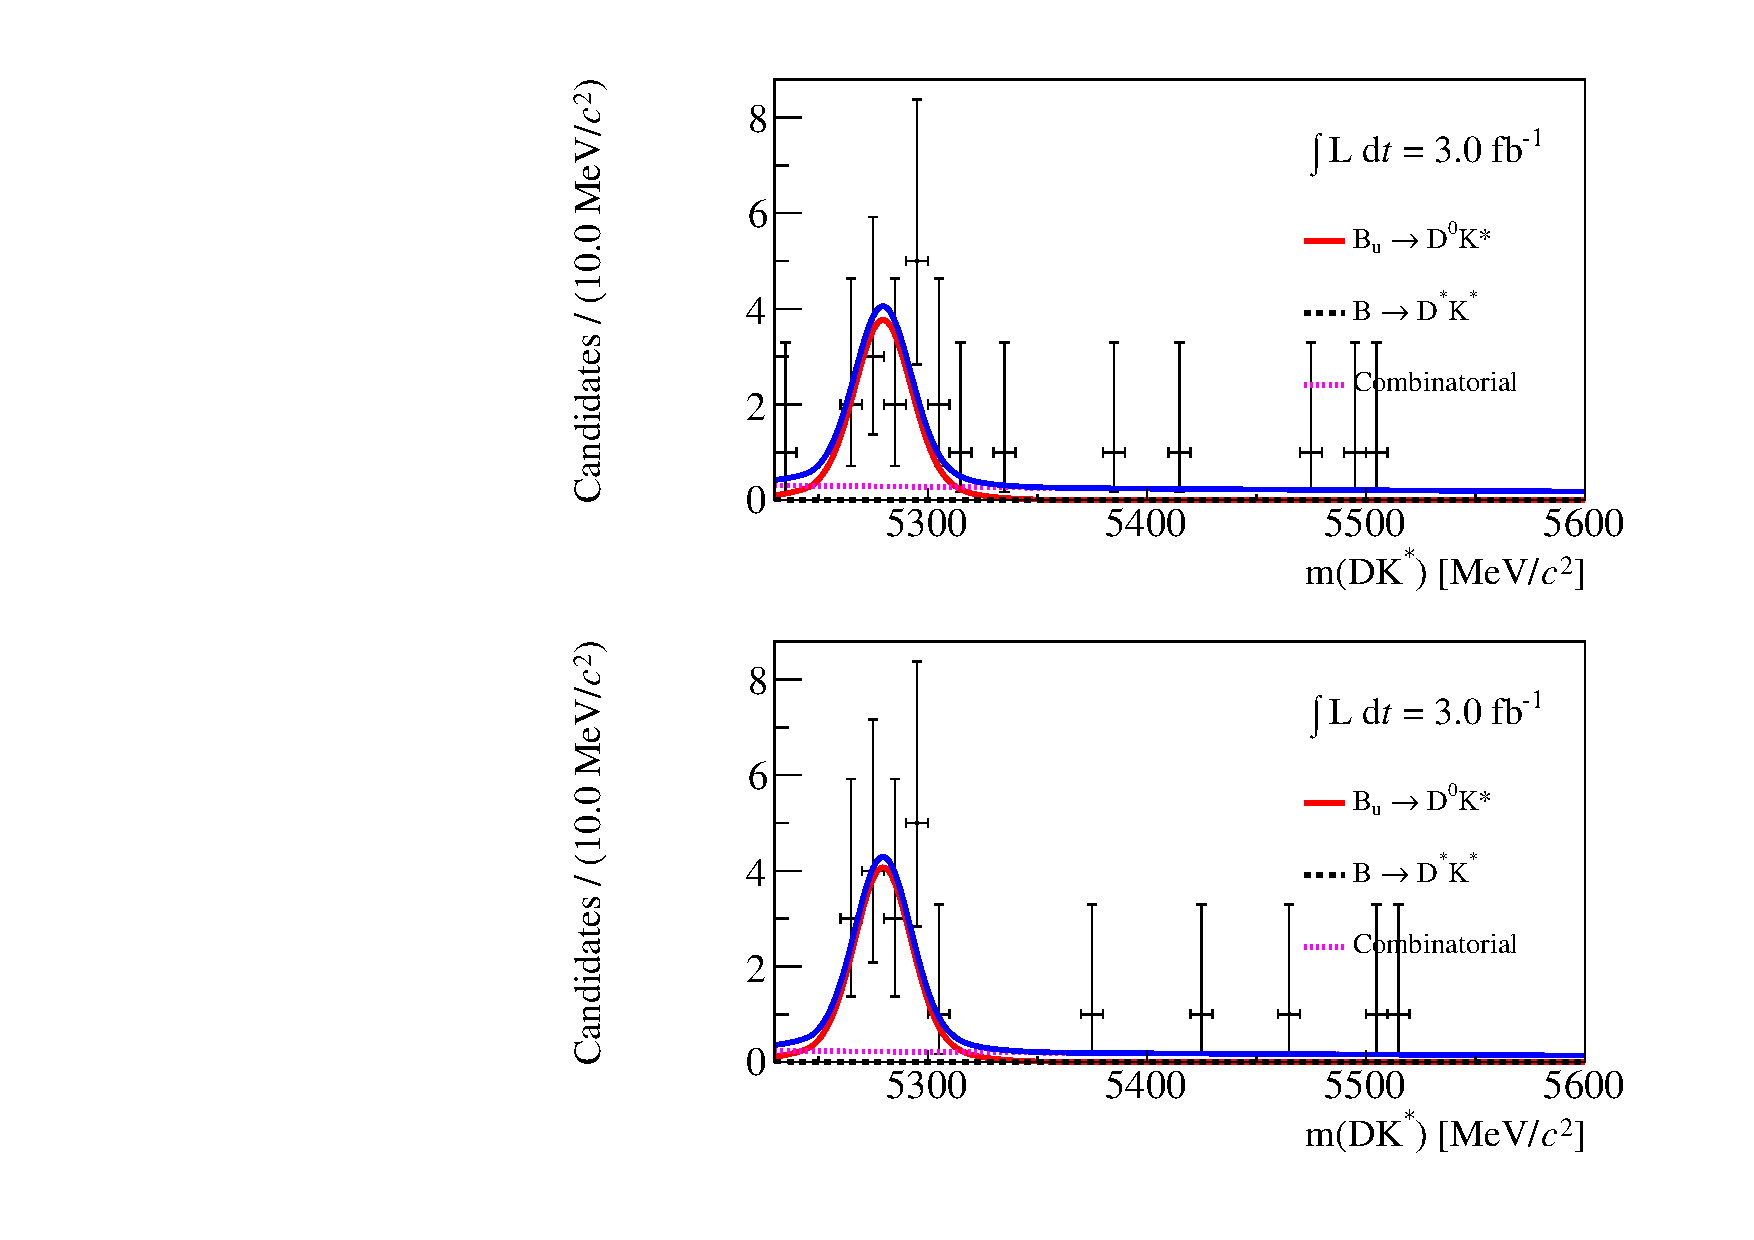
\includegraphics[width=0.3\linewidth]{figures/results/canvas_d2pipipipi_DD_run1.pdf}}
\hfill
\subfloat[$\pi K\pi\pi$, DD]{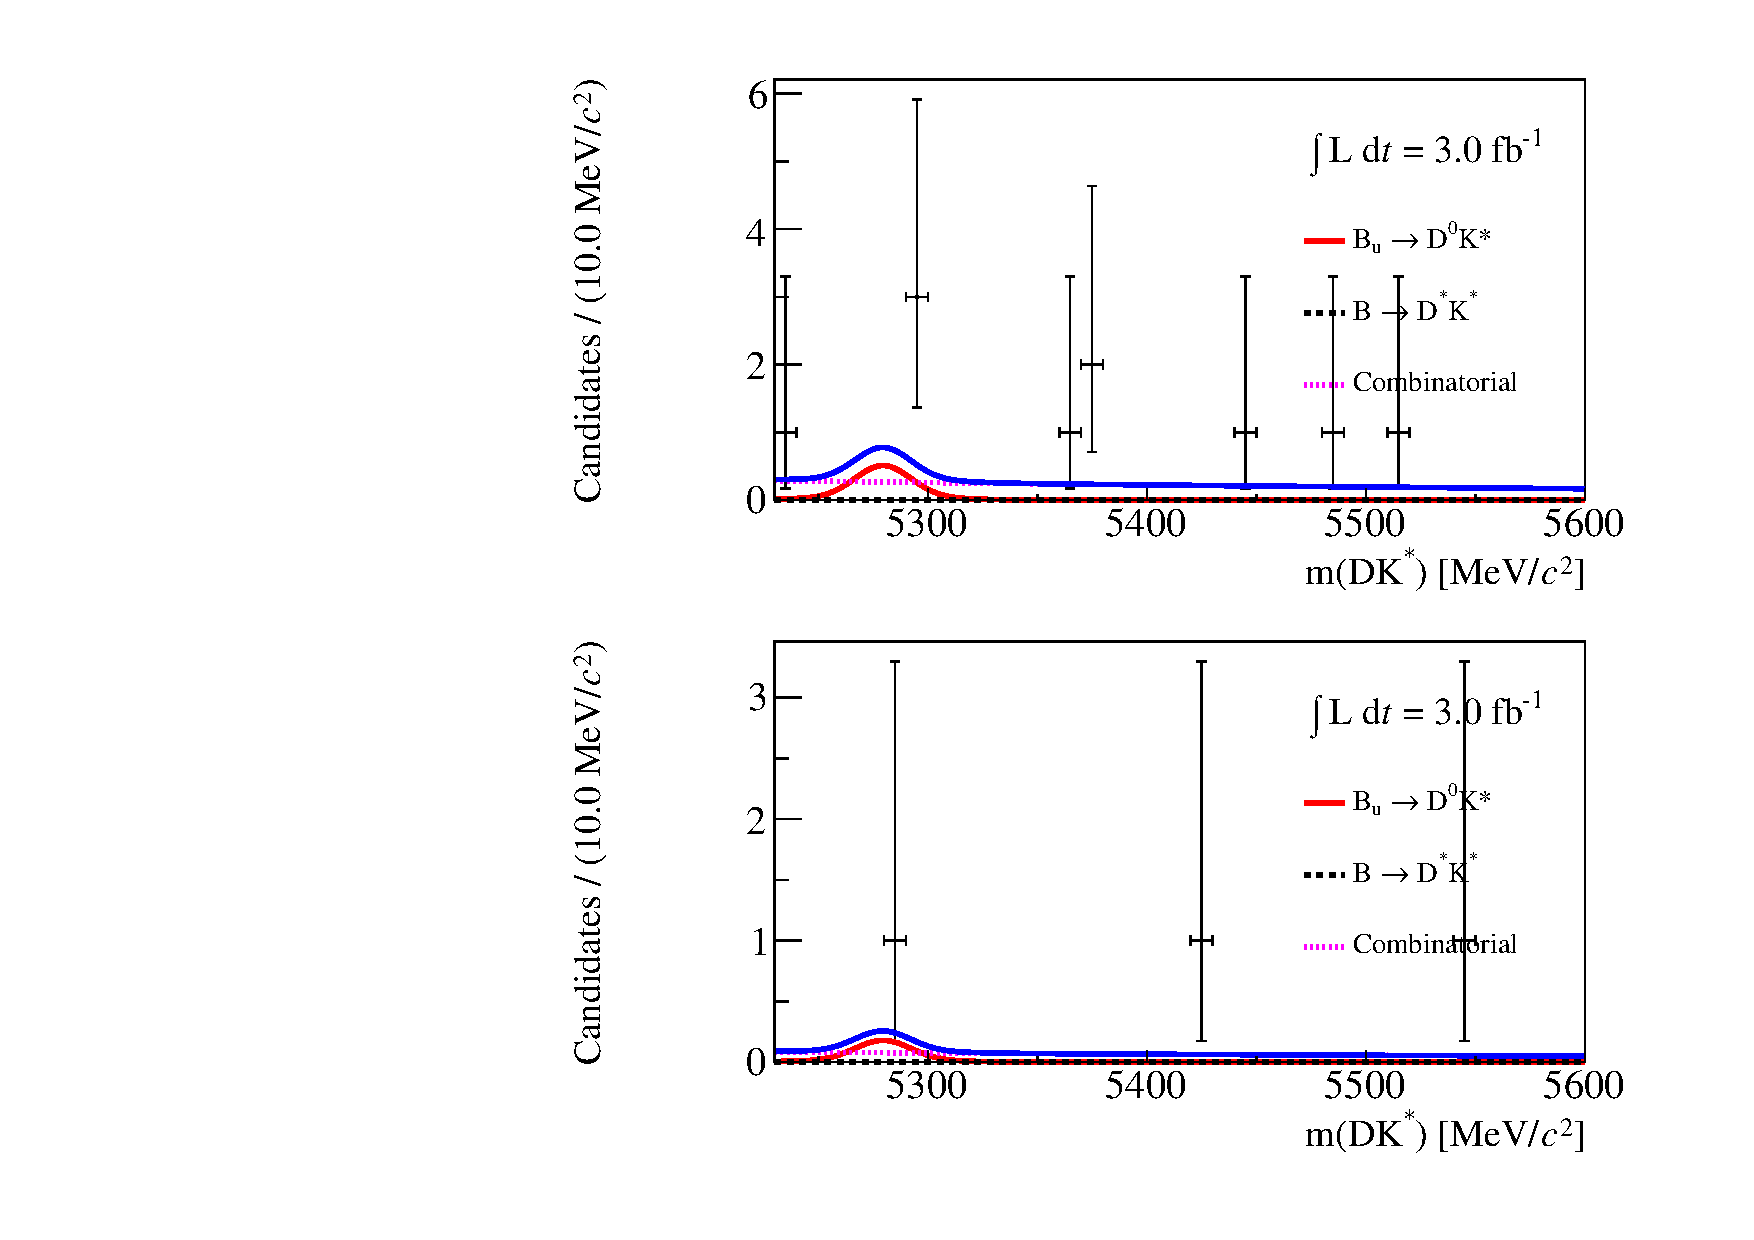
\includegraphics[width=0.3\linewidth]{figures/results/canvas_d2pikpipi_DD_run1.pdf}}
\caption{Results of the simultaneous fit for Run 1 data for 4-body modes. In each pair the top plot is for \Bp decays and the bottom plot is for \Bm decays.}
\label{datafit4bodyRun1}
\end{sidewaysfigure}

\begin{sidewaysfigure}[h]
\centering
\subfloat[$K\pi$, LL]{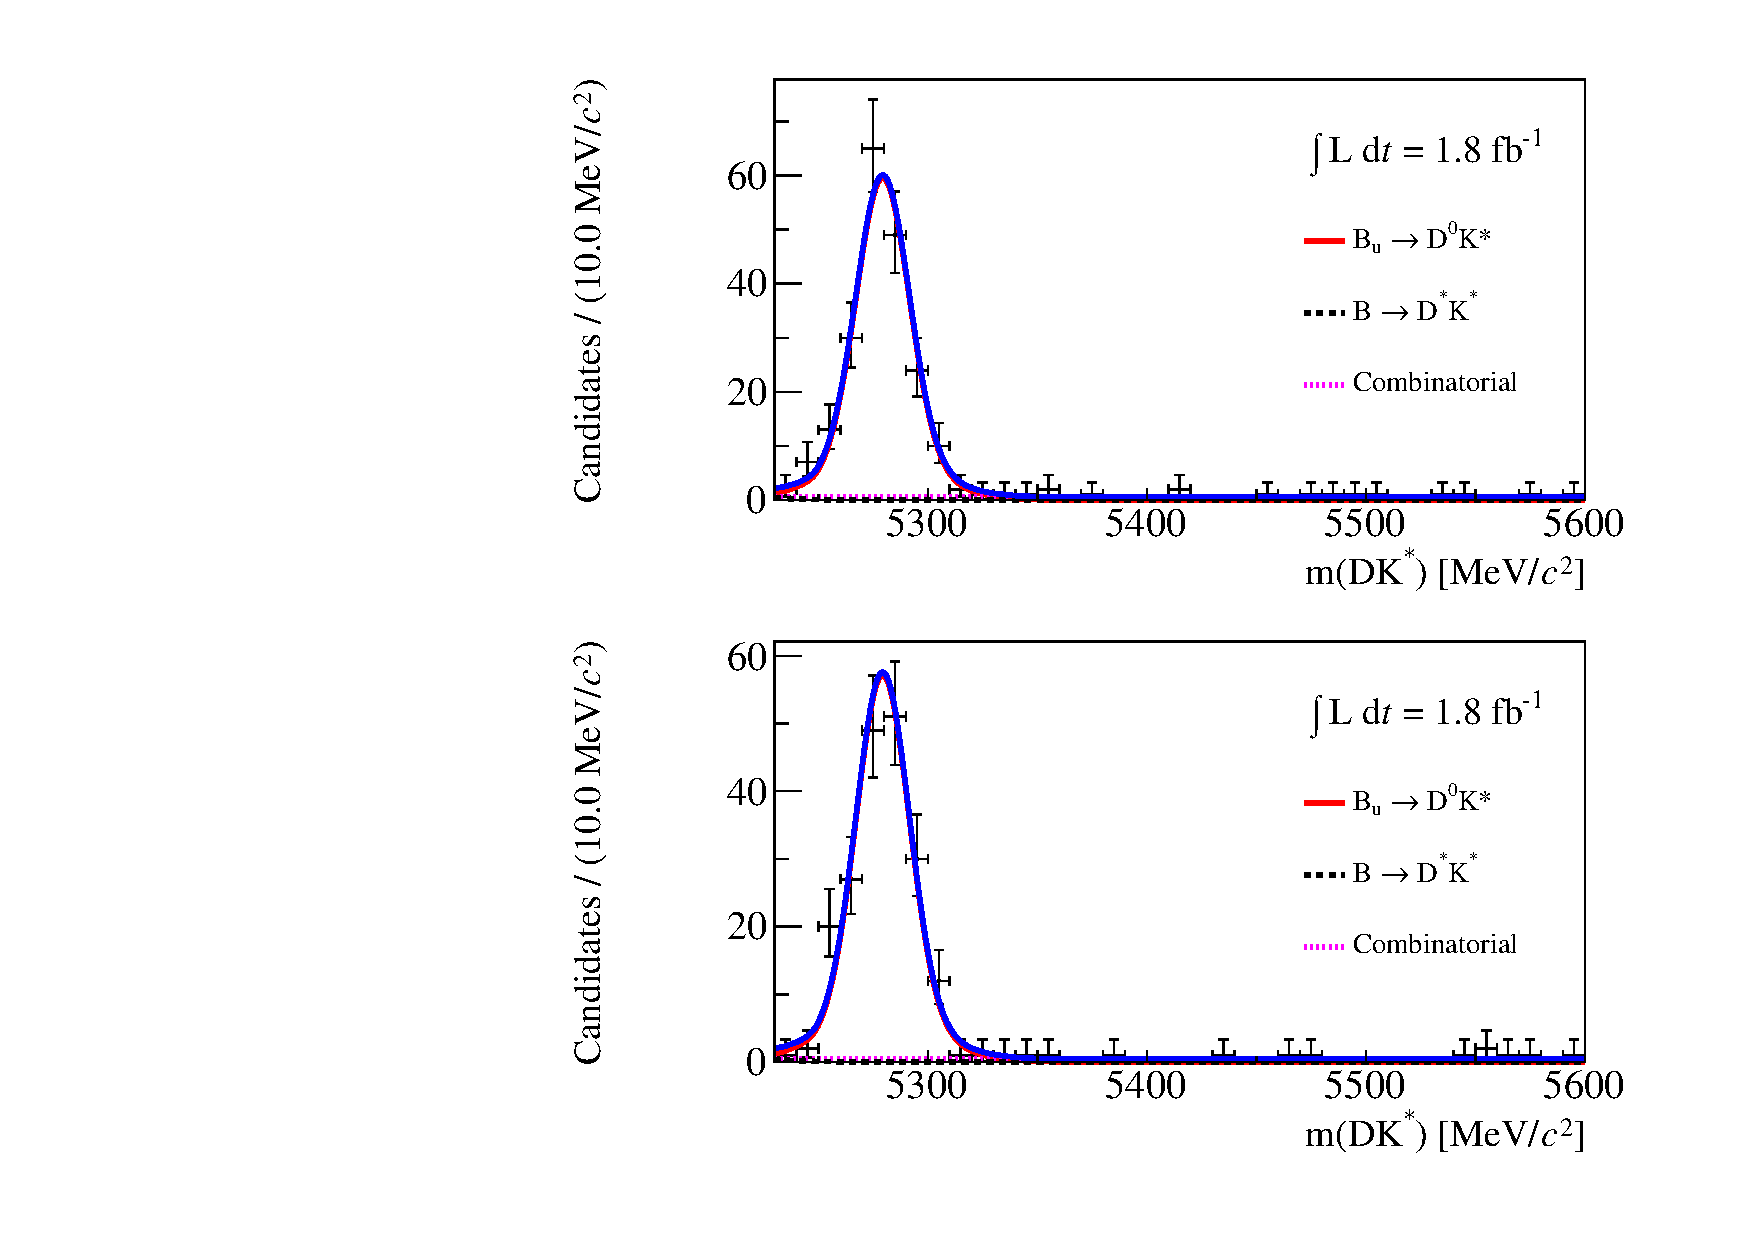
\includegraphics[width=0.25\linewidth]{figures/results/canvas_d2kpi_LL_run2.pdf}}
\hfill
\subfloat[$KK$, LL]{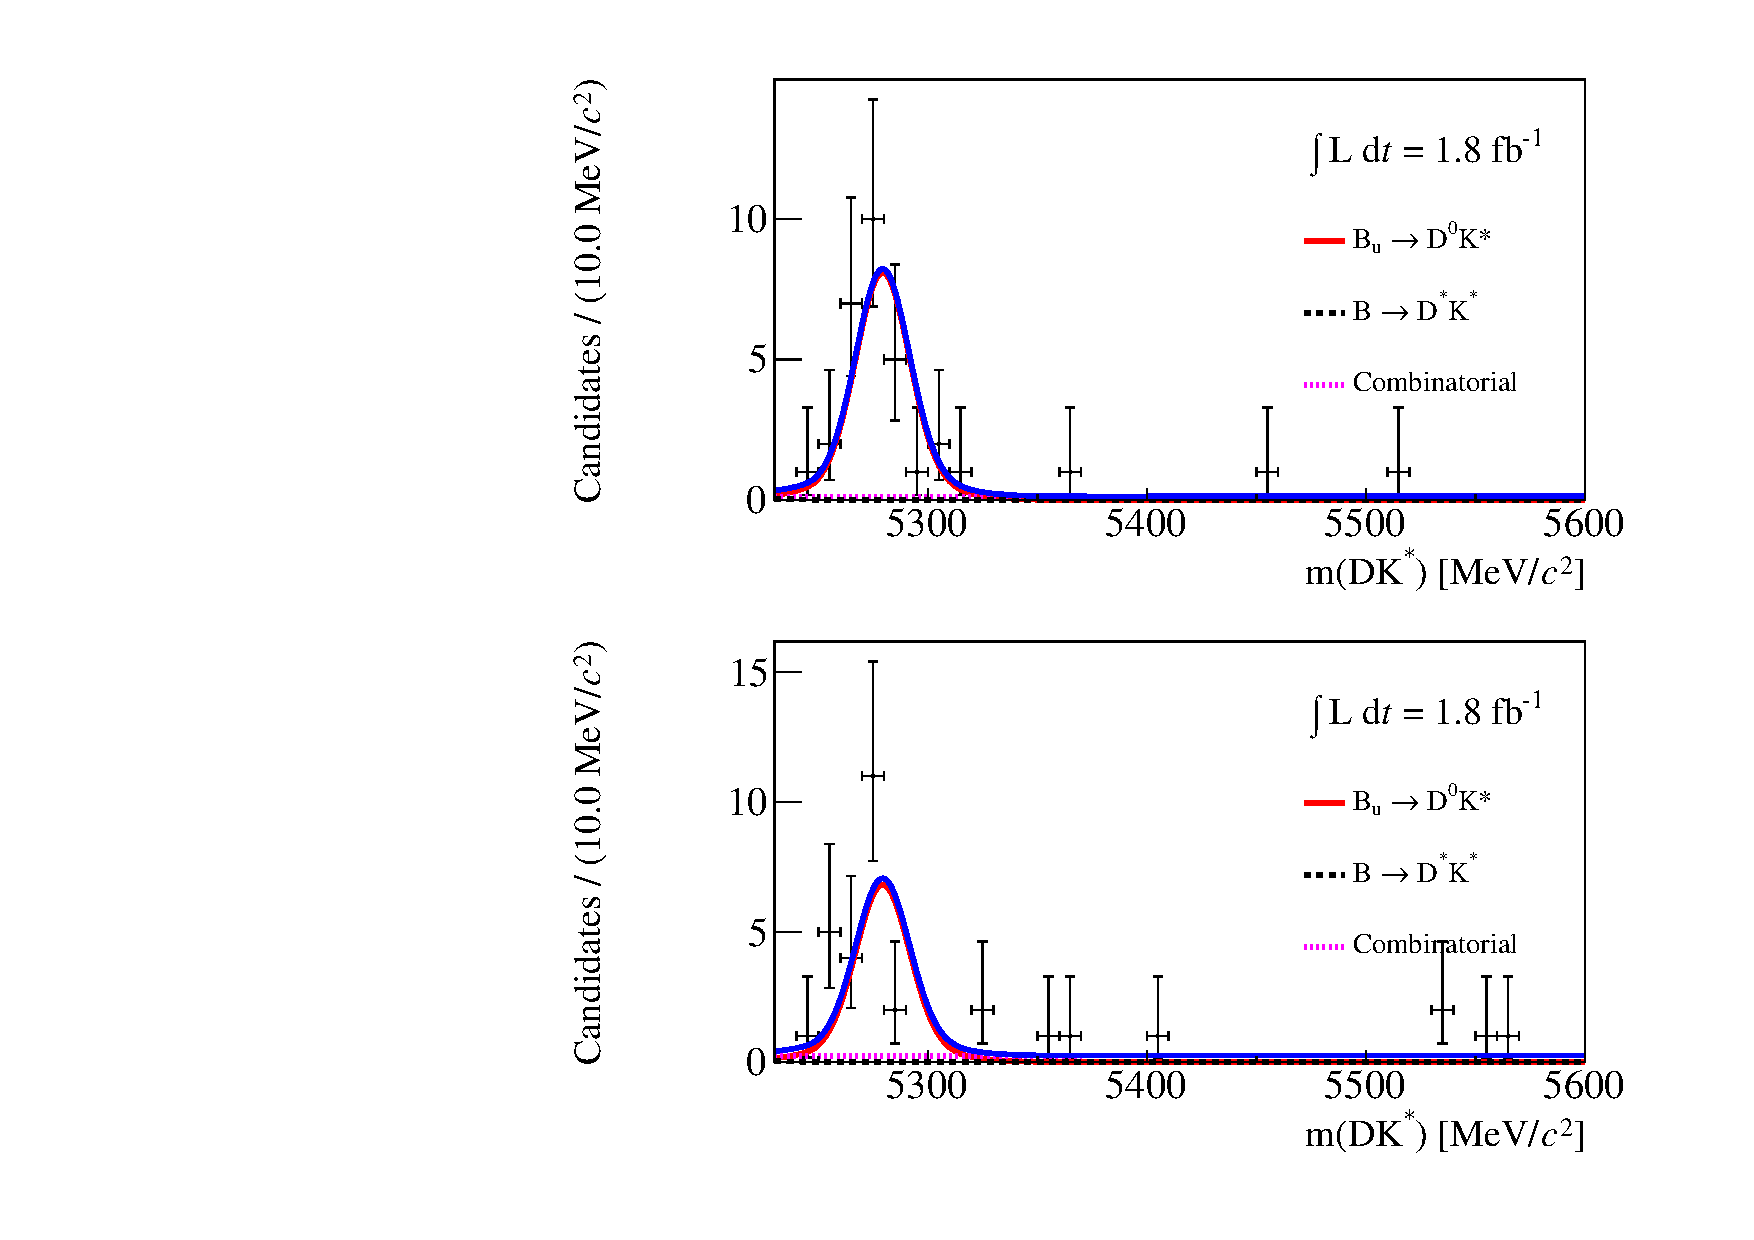
\includegraphics[width=0.25\linewidth]{figures/results/canvas_d2kk_LL_run2.pdf}}
\hfill
\subfloat[$\pi\pi$, LL]{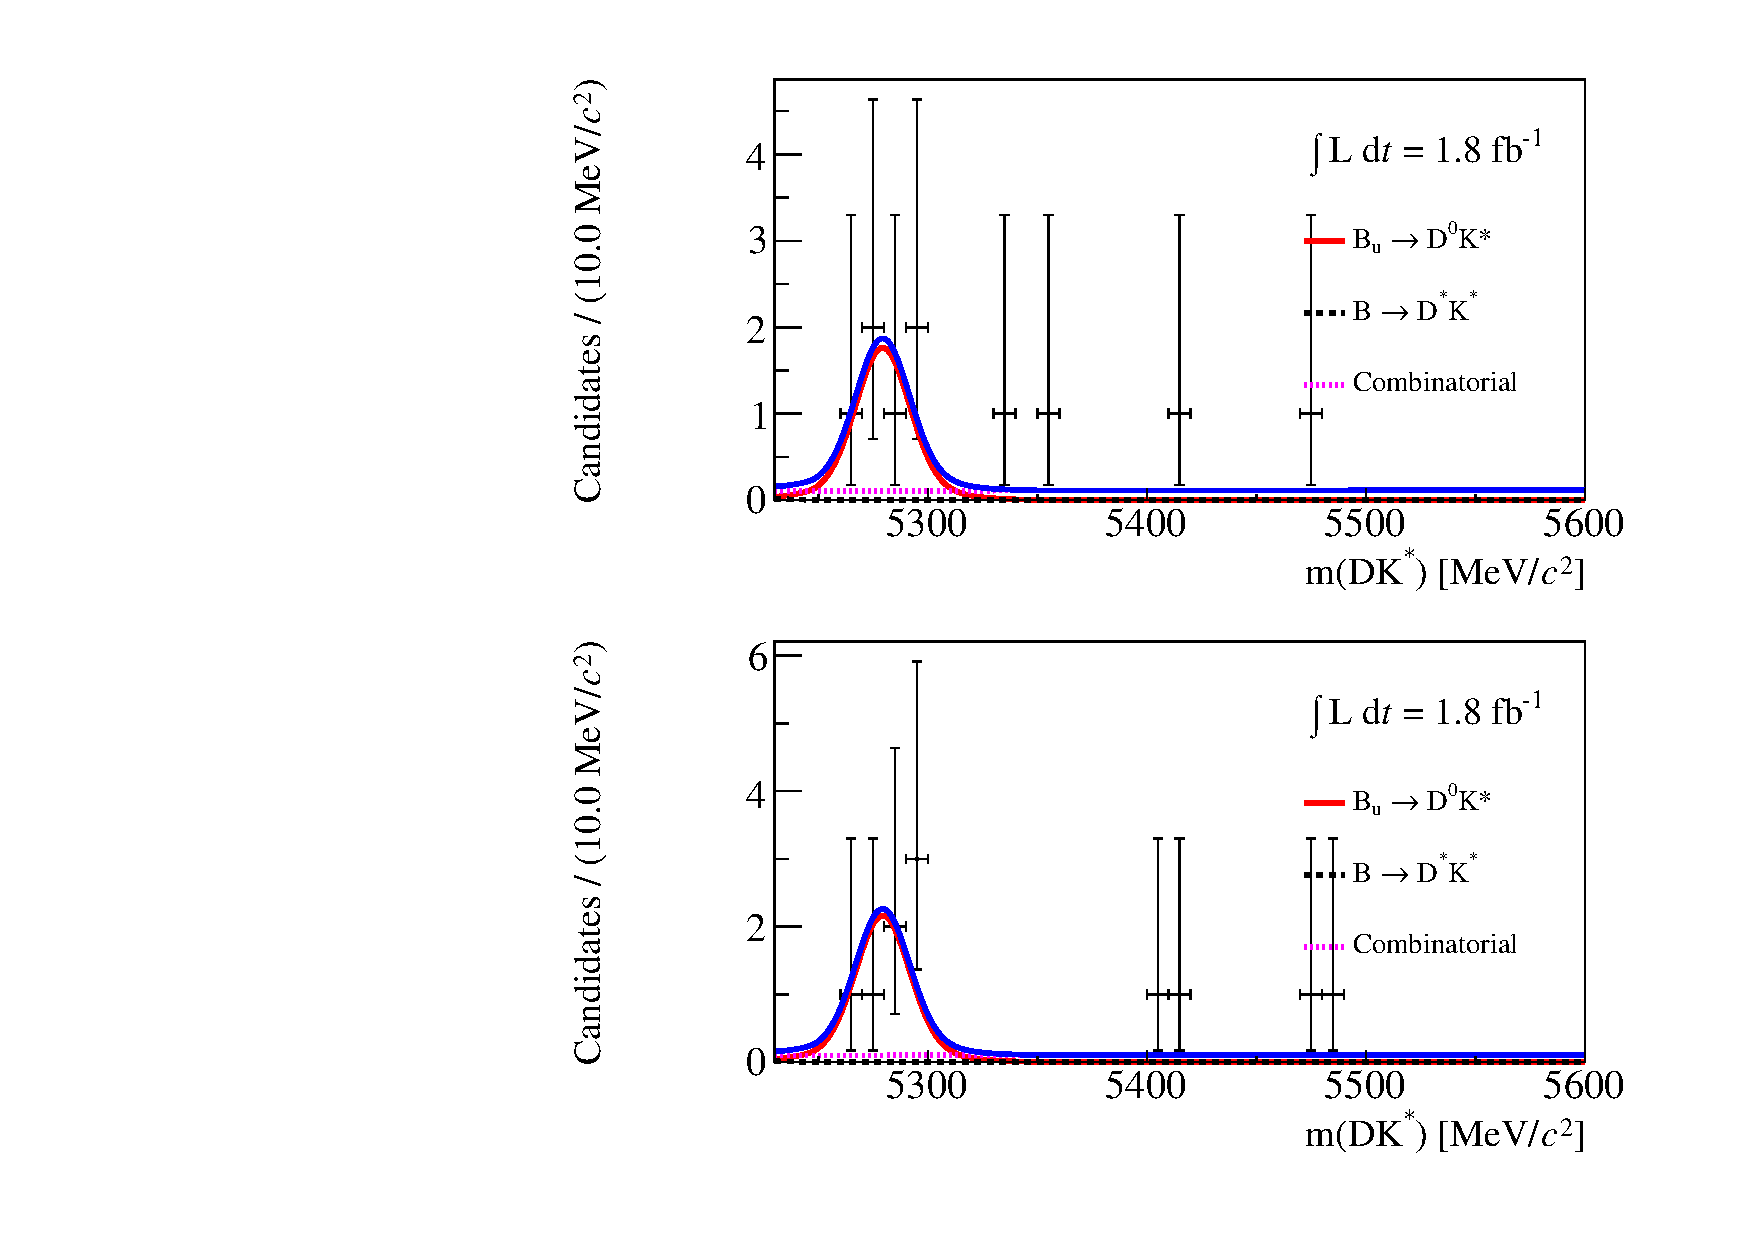
\includegraphics[width=0.25\linewidth]{figures/results/canvas_d2pipi_LL_run2.pdf}}
\hfill
\subfloat[$\pi K$, LL]{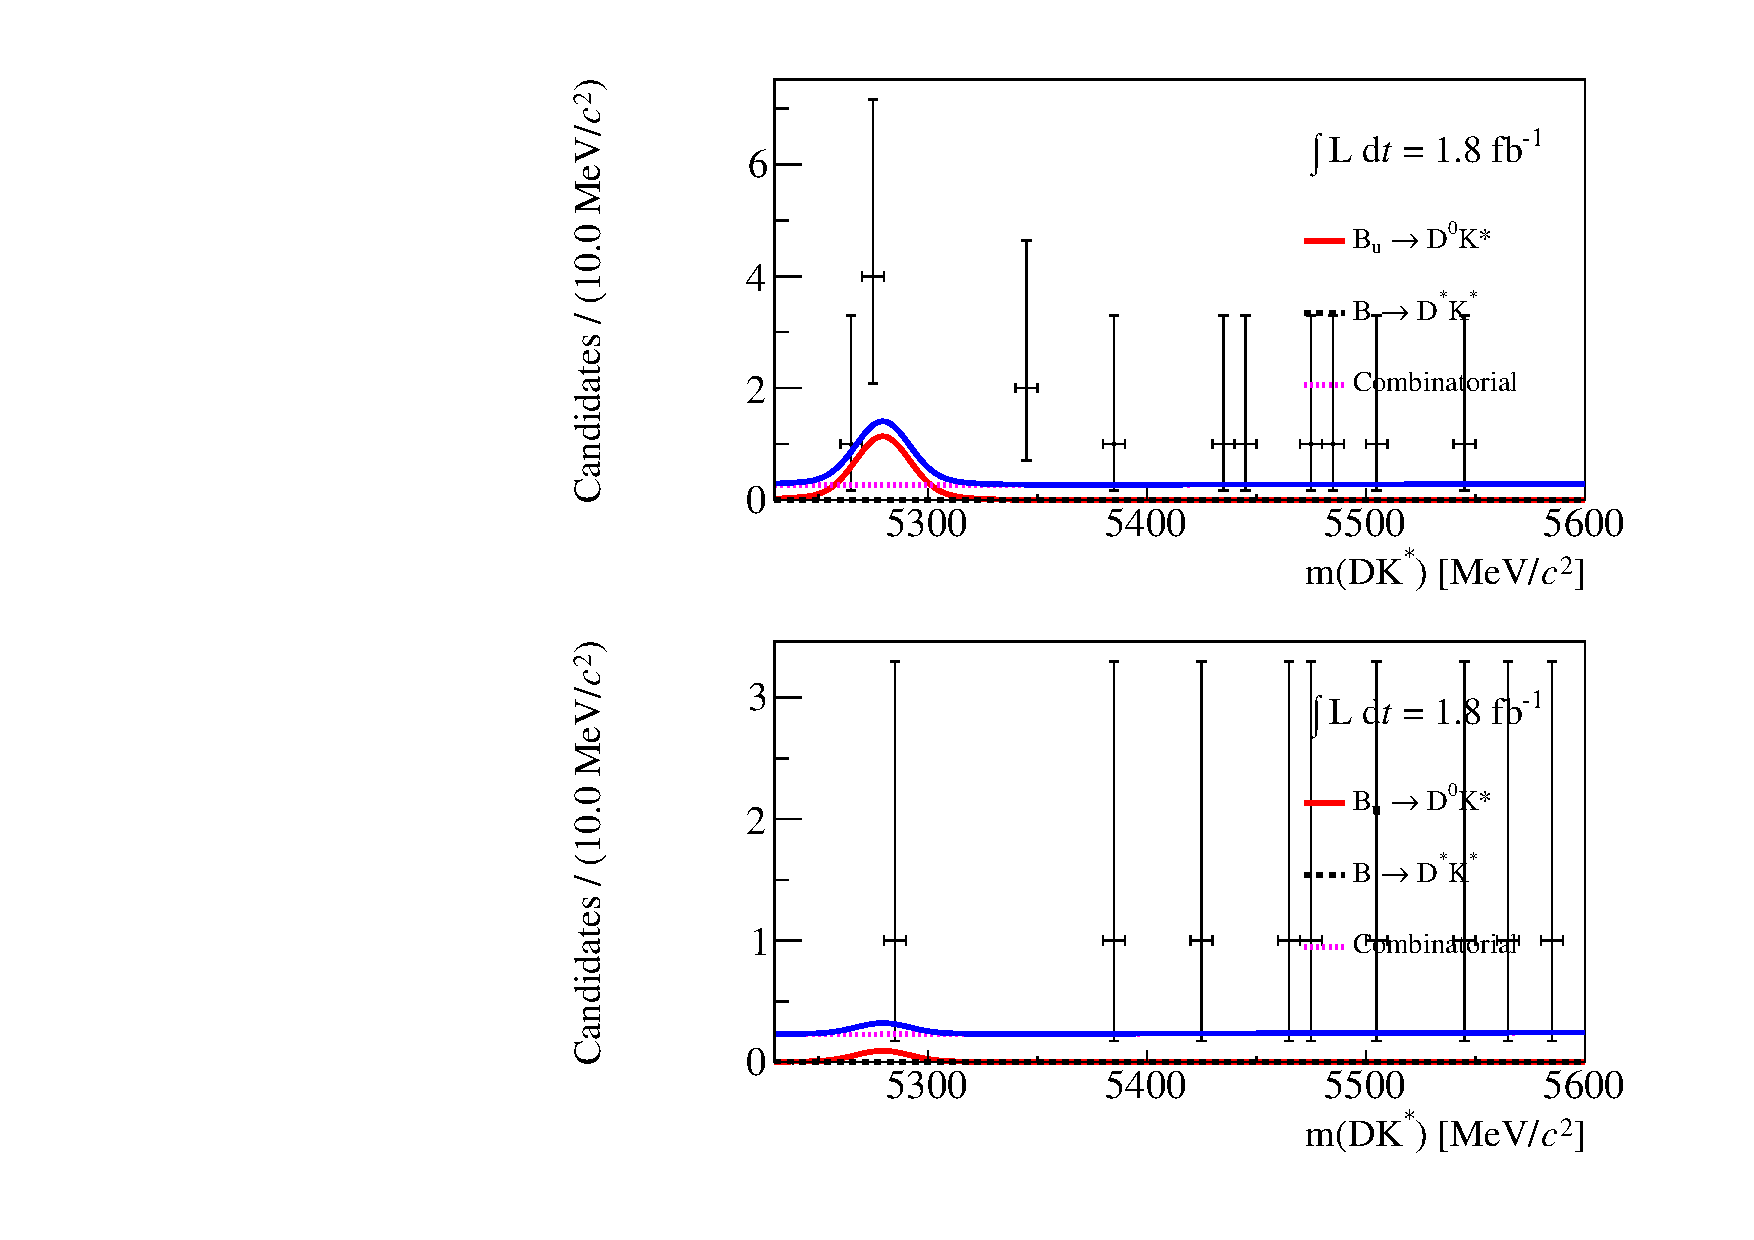
\includegraphics[width=0.25\linewidth]{figures/results/canvas_d2pik_LL_run2.pdf}}
\hfill
\subfloat[$K\pi$, DD]{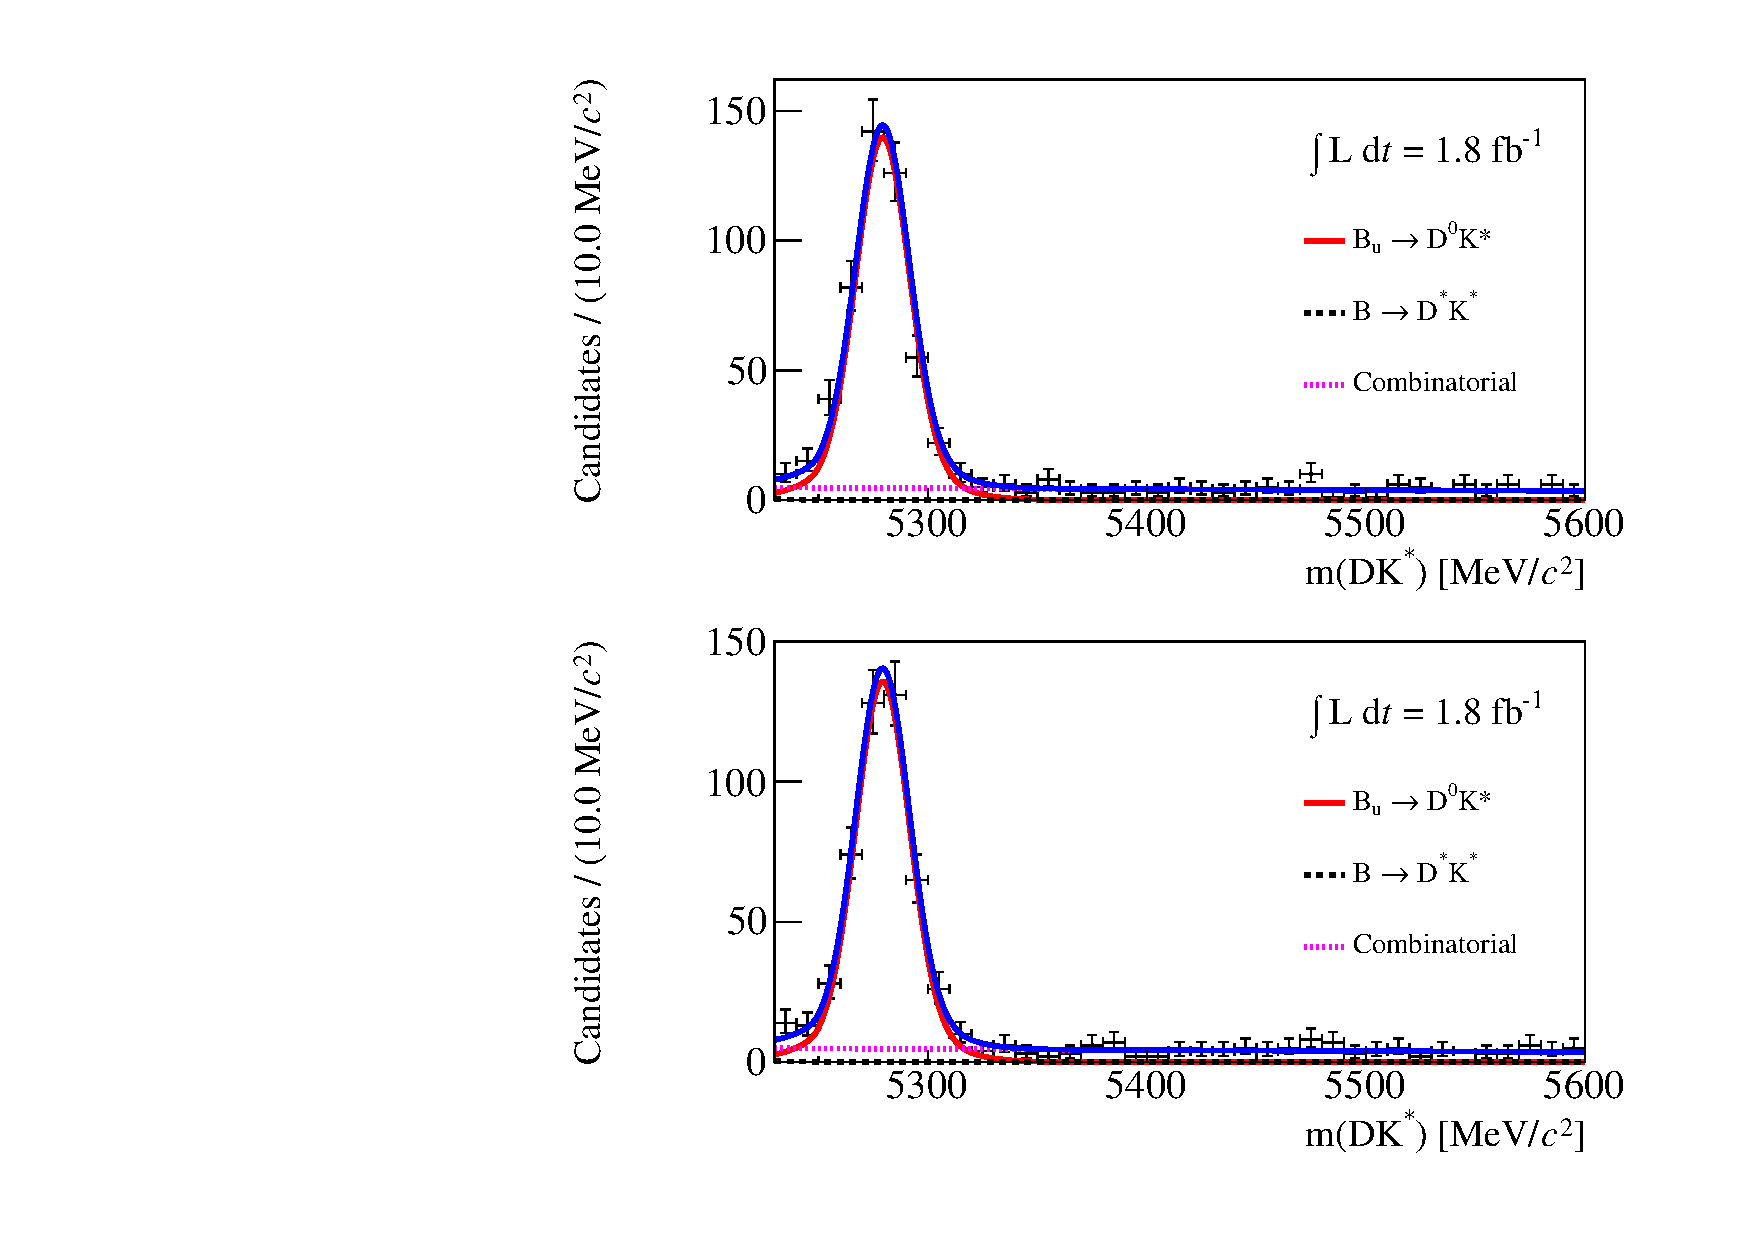
\includegraphics[width=0.25\linewidth]{figures/results/canvas_d2kpi_DD_run2.pdf}}
\hfill
\subfloat[$KK$, DD]{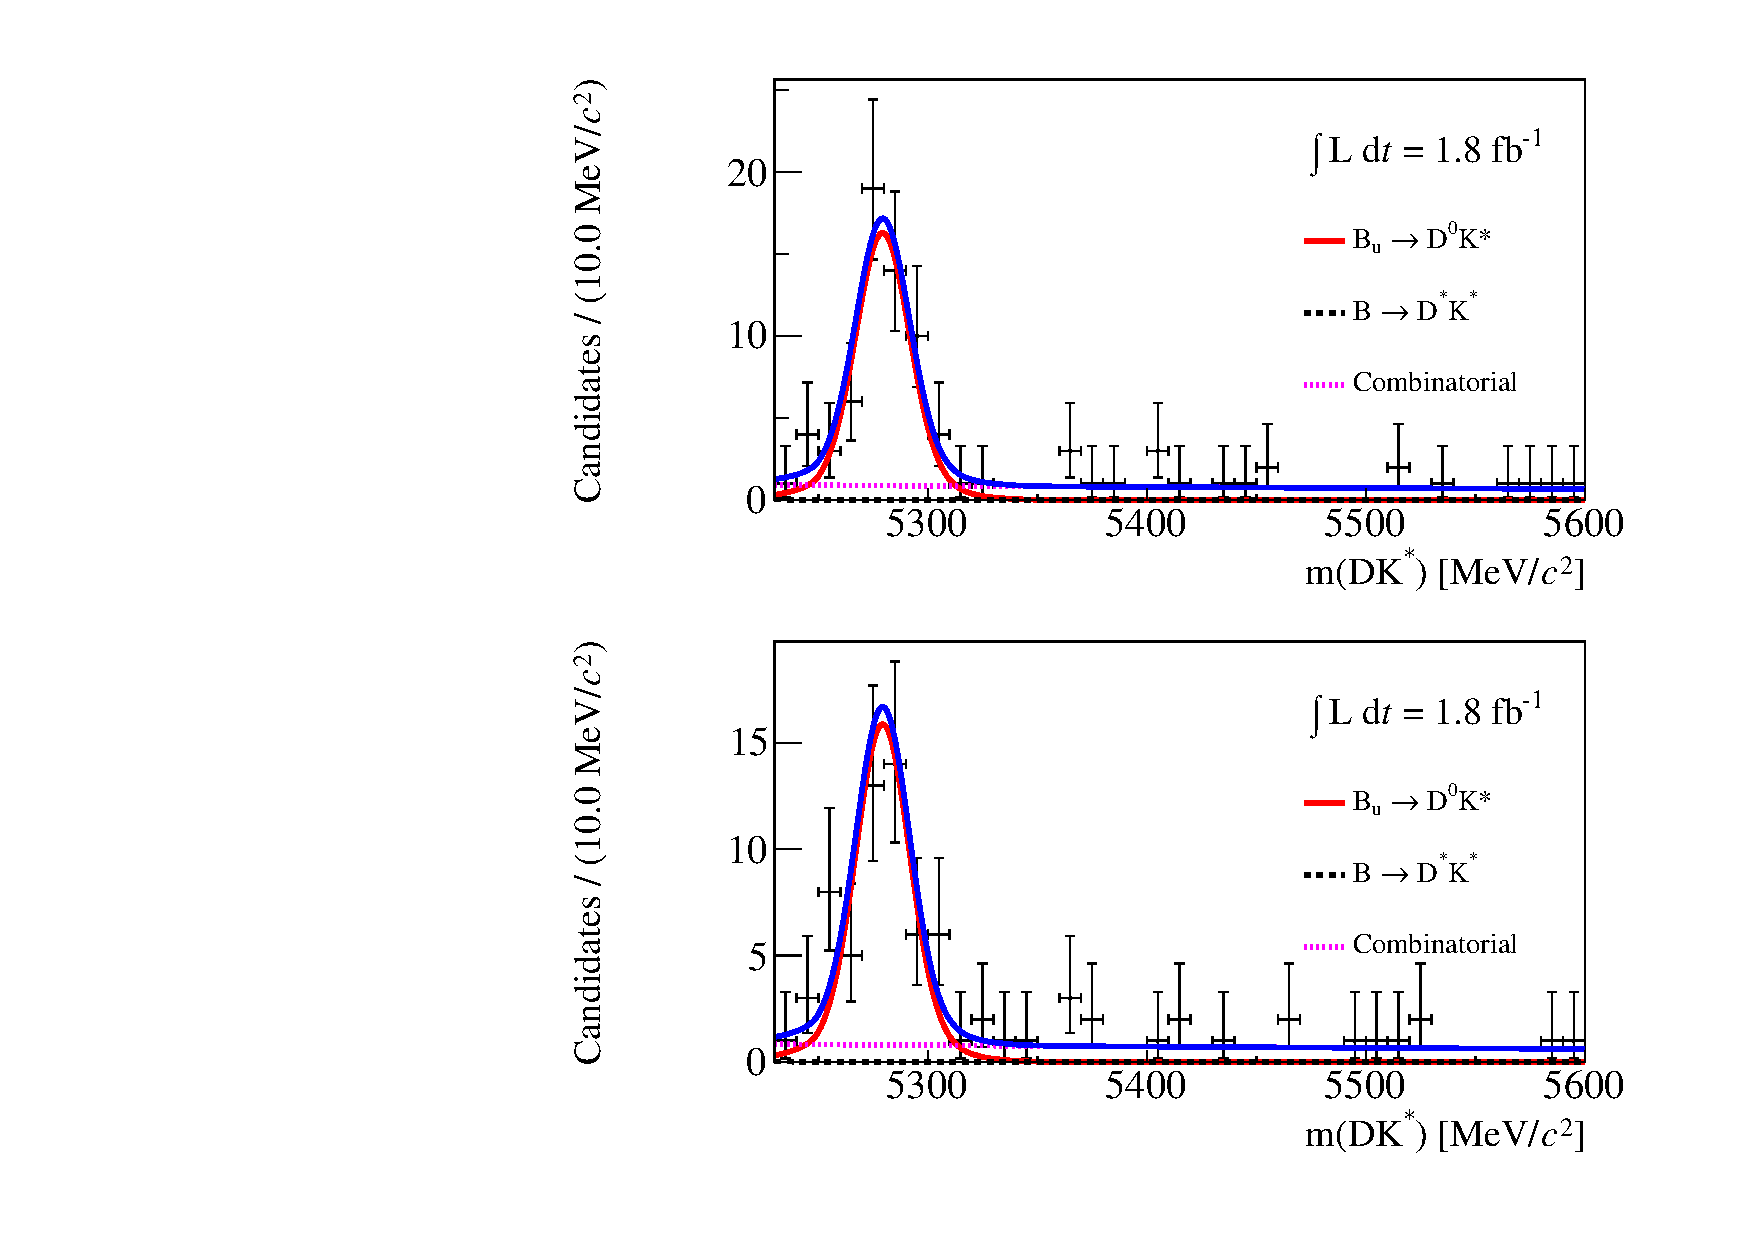
\includegraphics[width=0.25\linewidth]{figures/results/canvas_d2kk_DD_run2.pdf}}
\hfill
\subfloat[$\pi\pi$, DD]{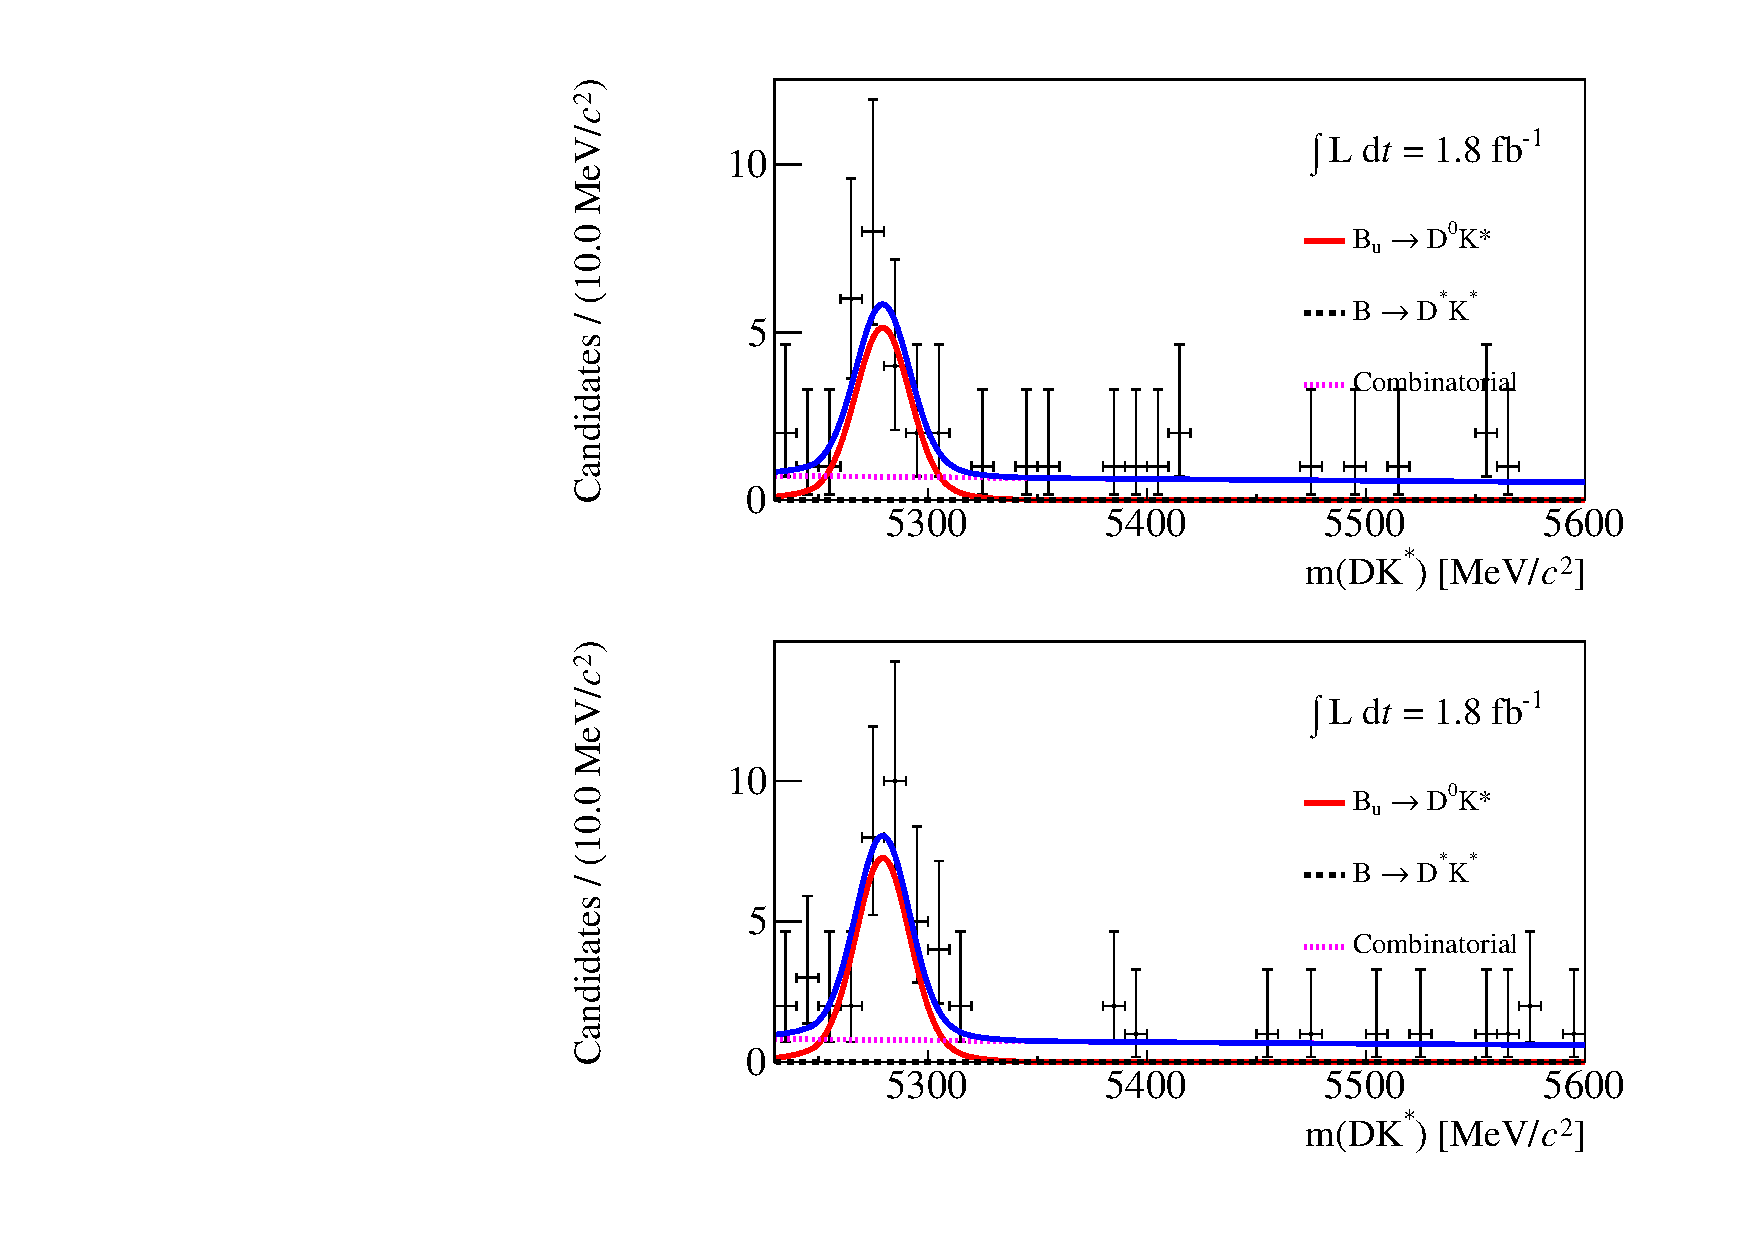
\includegraphics[width=0.25\linewidth]{figures/results/canvas_d2pipi_DD_run2.pdf}}
\hfill
\subfloat[$\pi K$, DD]{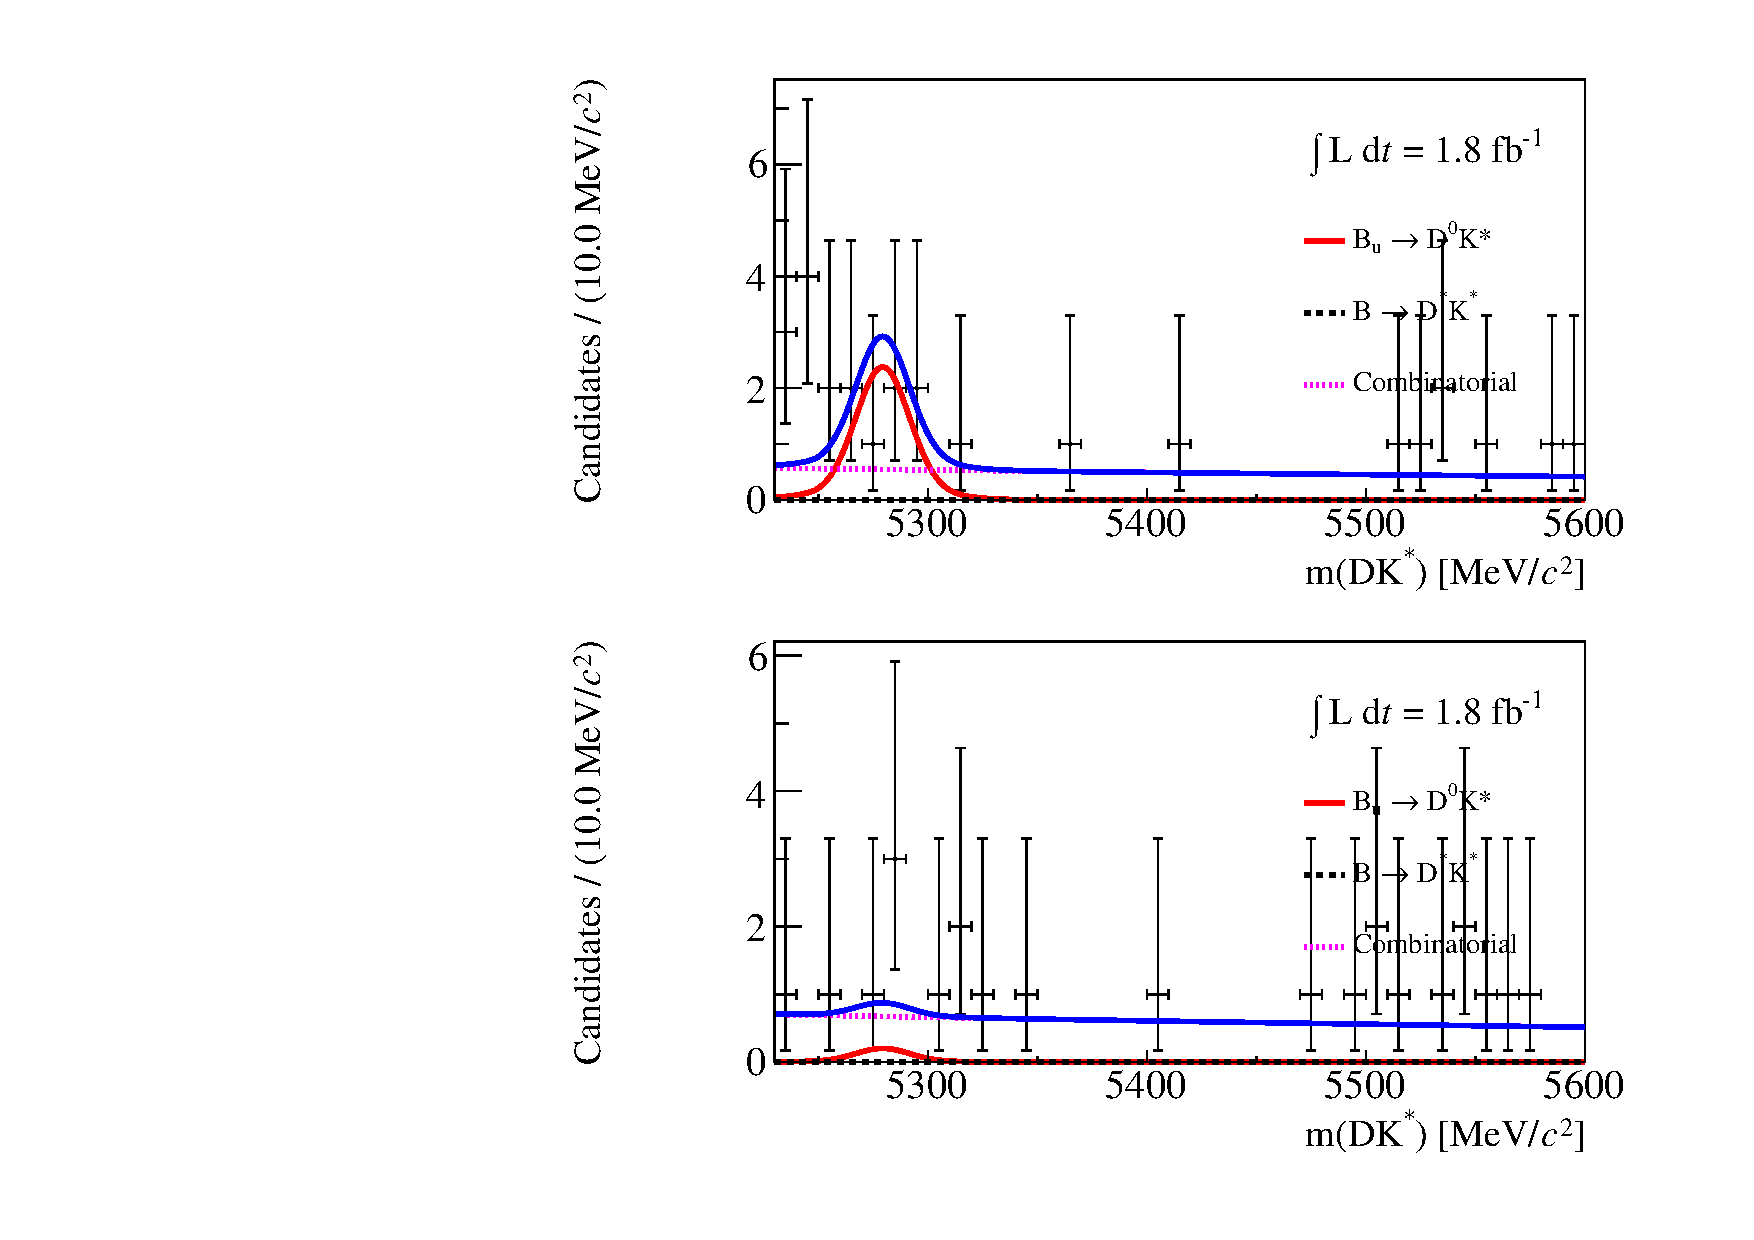
\includegraphics[width=0.25\linewidth]{figures/results/canvas_d2pik_DD_run2.pdf}}
\caption{Results of the simultaneous fit for Run 1 data for 2-body modes. In each pair the top plot is for \Bp decays and the bottom plot is for \Bm decays.}
\label{datafit2bodyRun2}
\end{sidewaysfigure}

\begin{sidewaysfigure}[h]
\centering
\subfloat[$K\pi\pi\pi$, LL]{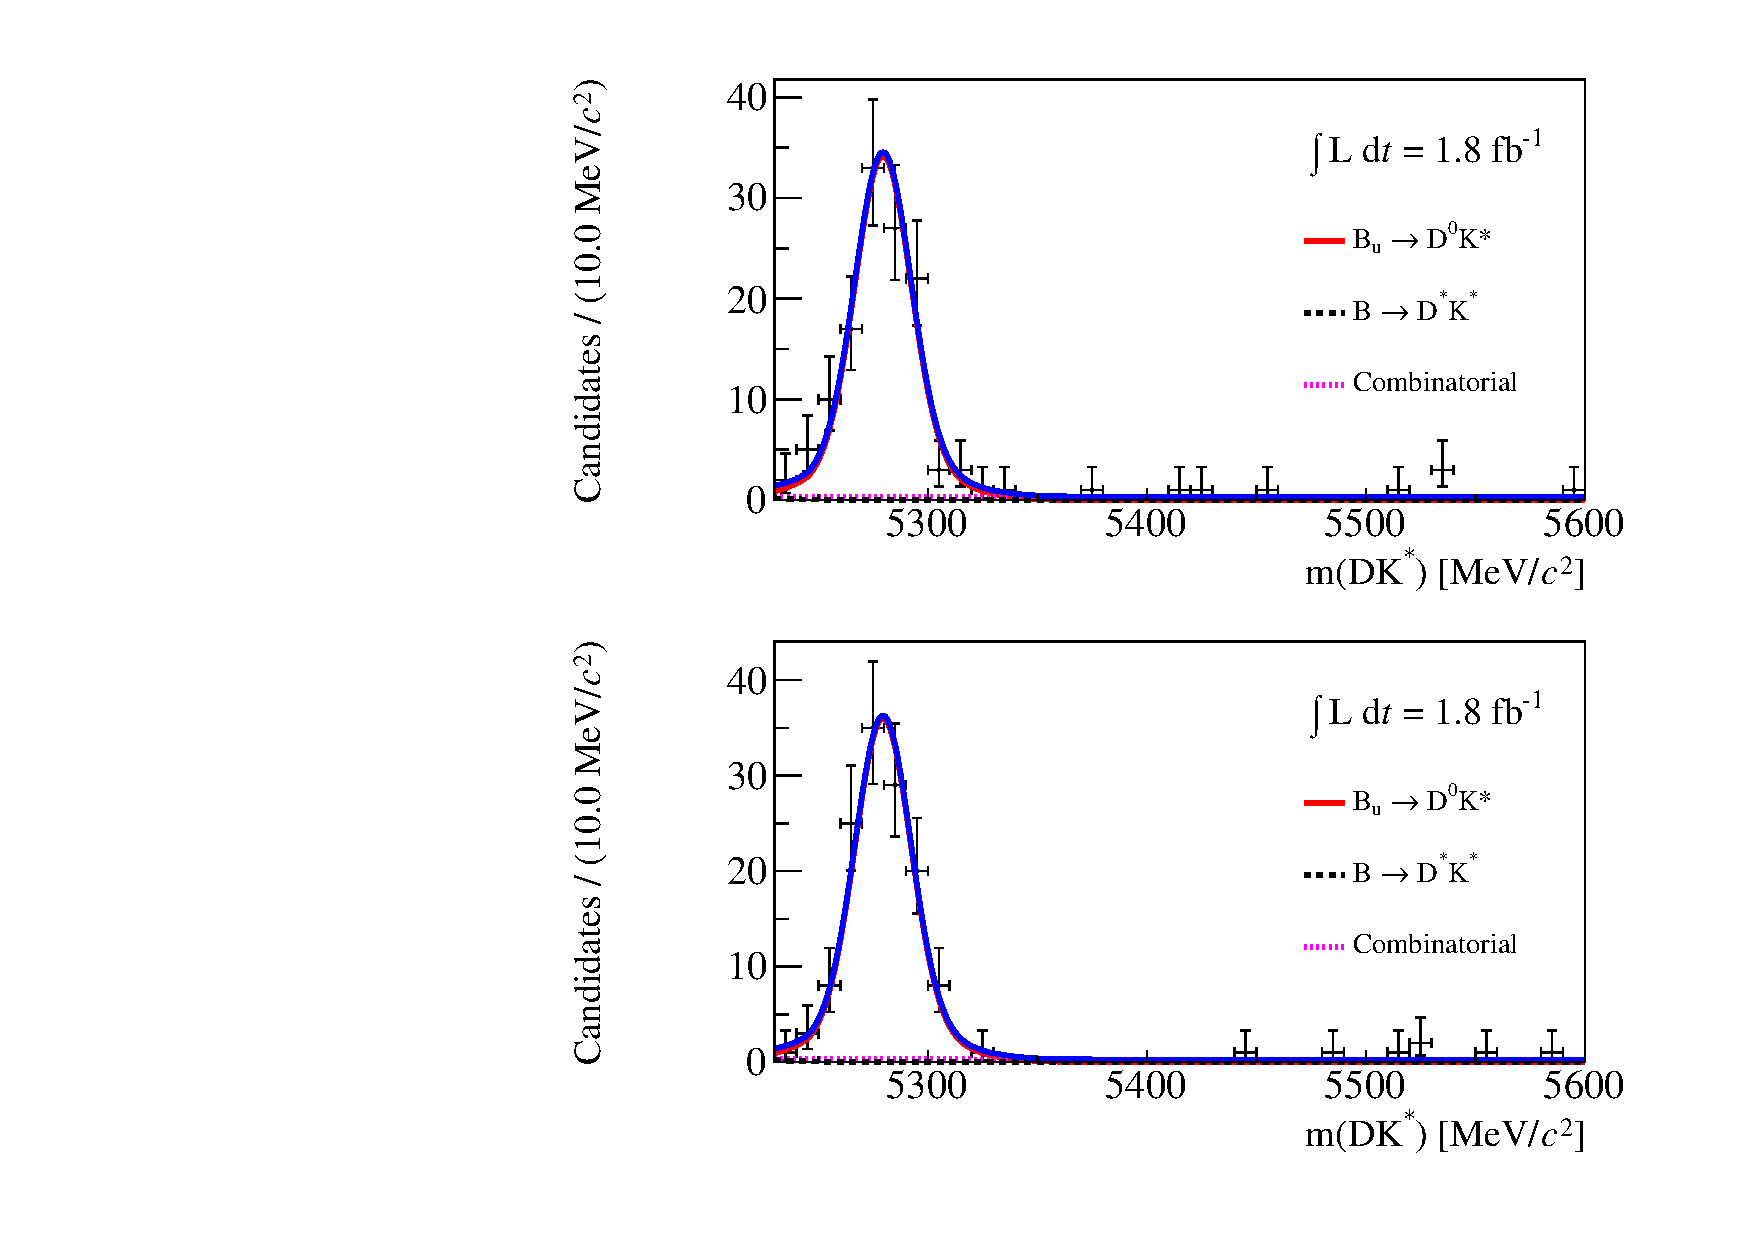
\includegraphics[width=0.3\linewidth]{figures/results/canvas_d2kpipipi_LL_run2.pdf}}
\hfill
\subfloat[$\pi\pi\pi\pi$, LL]{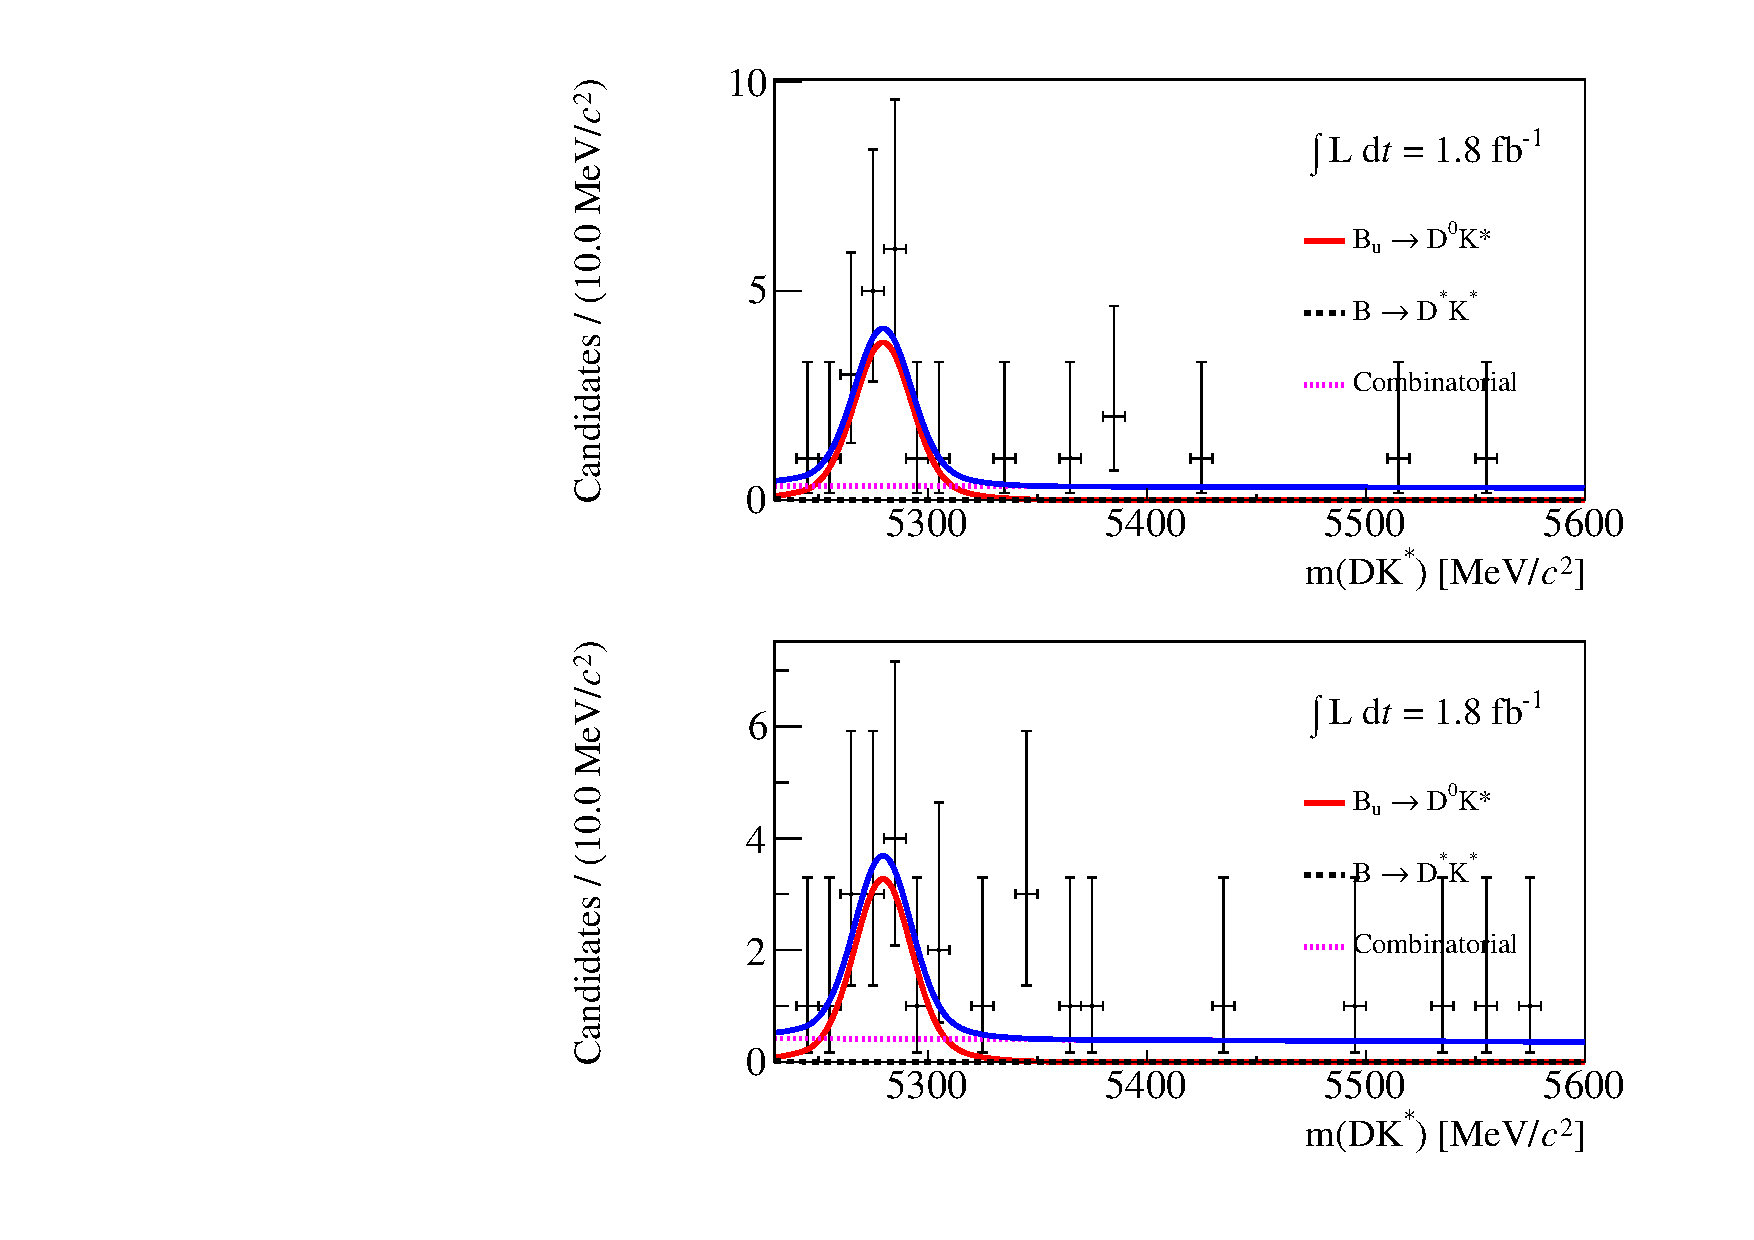
\includegraphics[width=0.3\linewidth]{figures/results/canvas_d2pipipipi_LL_run2.pdf}}
\hfill
\subfloat[$\pi K\pi\pi$, LL]{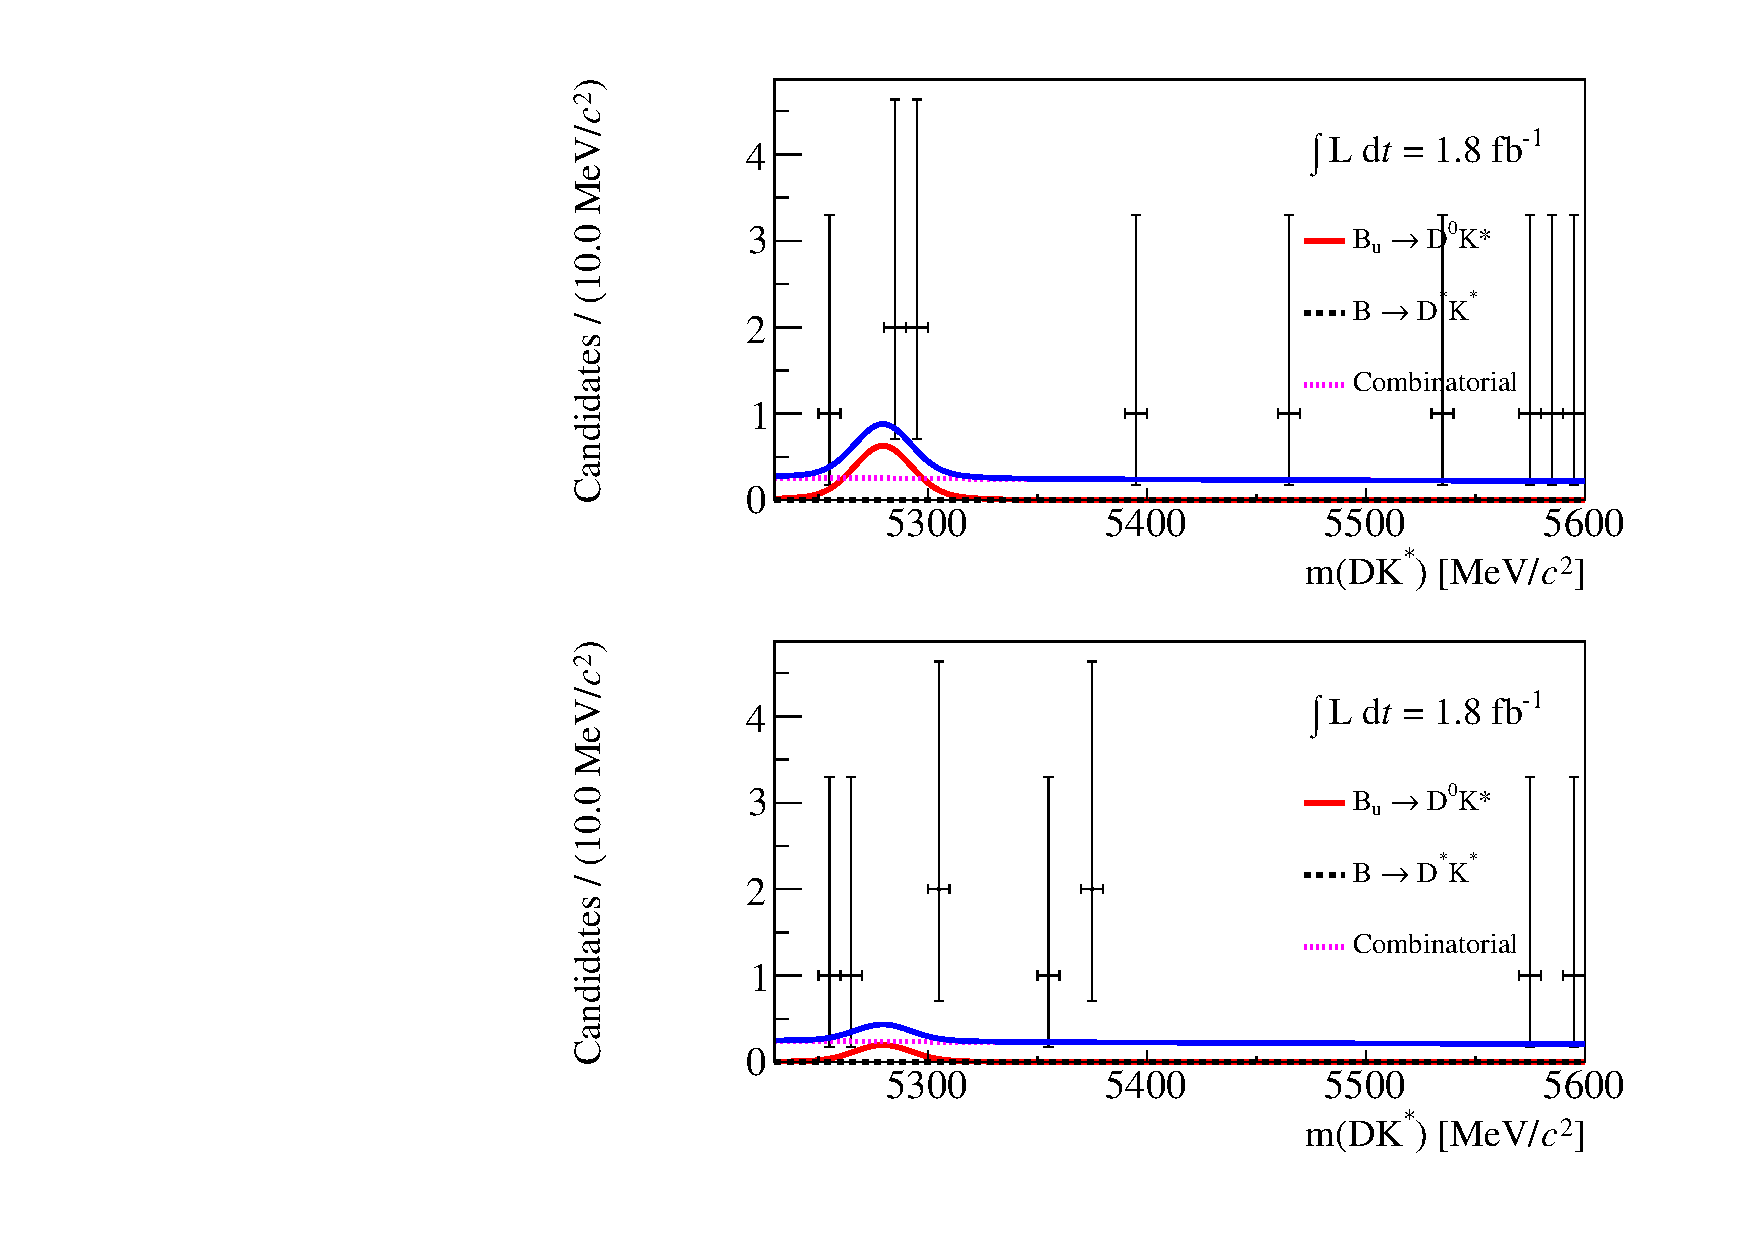
\includegraphics[width=0.3\linewidth]{figures/results/canvas_d2pikpipi_LL_run2.pdf}}
\hfill
\subfloat[$K\pi\pi\pi$, DD]{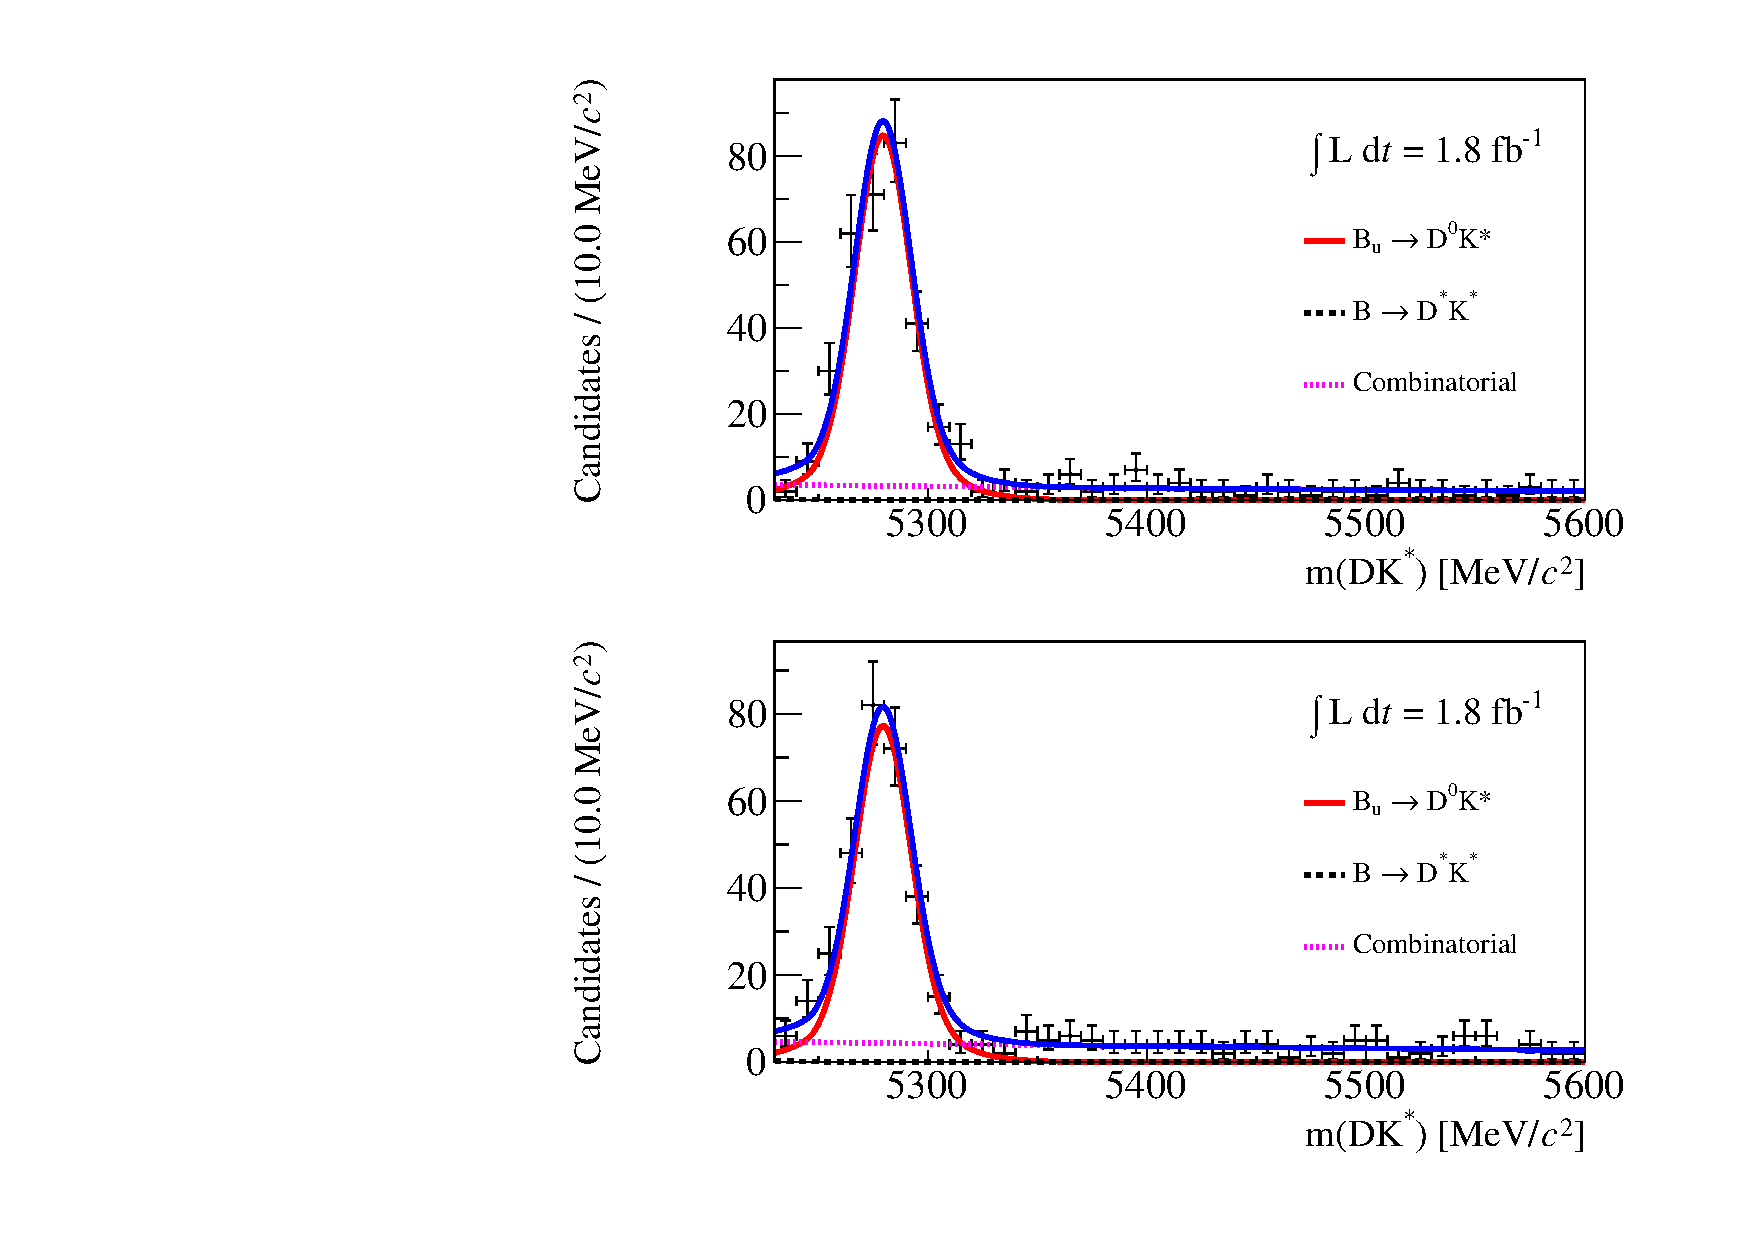
\includegraphics[width=0.3\linewidth]{figures/results/canvas_d2kpipipi_DD_run2.pdf}}
\hfill
\subfloat[$\pi\pi\pi\pi$, DD]{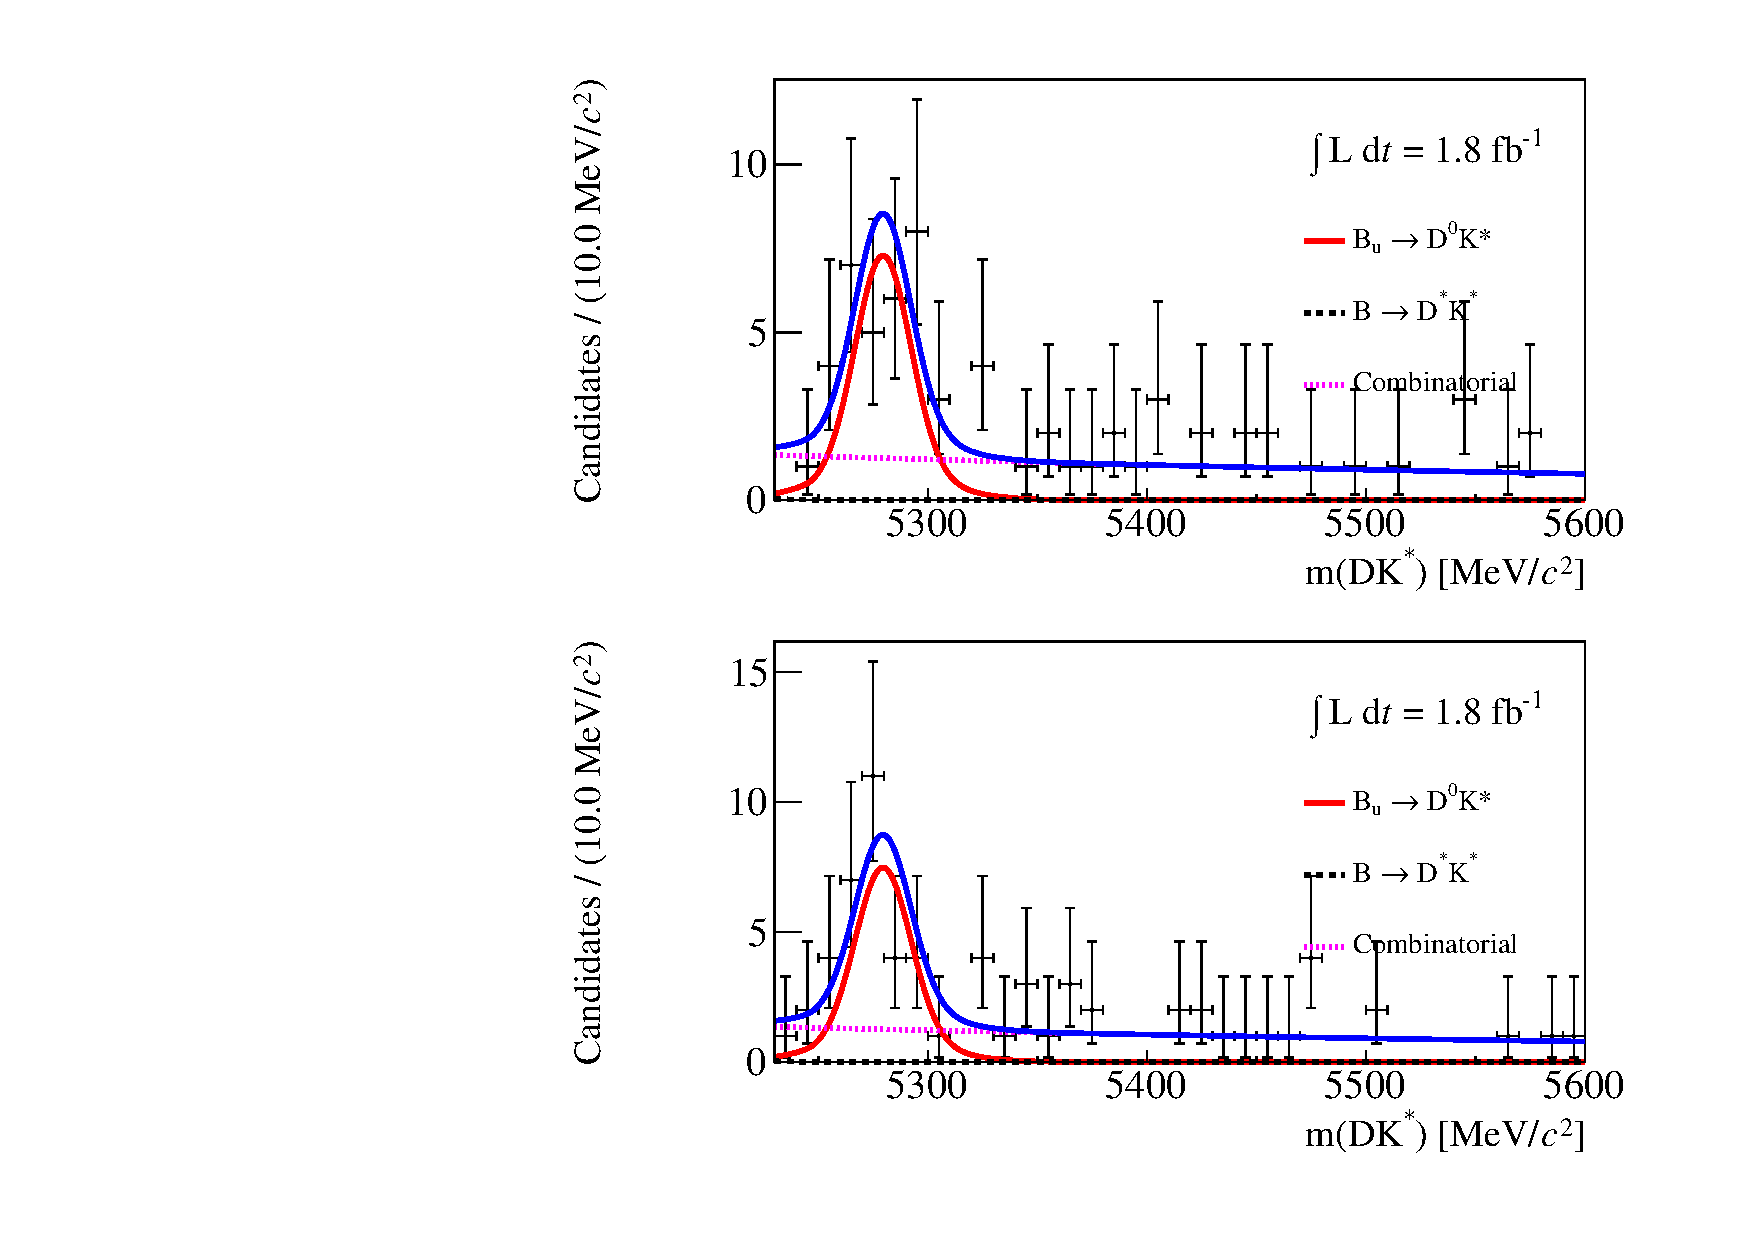
\includegraphics[width=0.3\linewidth]{figures/results/canvas_d2pipipipi_DD_run2.pdf}}
\hfill
\subfloat[$\pi K\pi\pi$, DD]{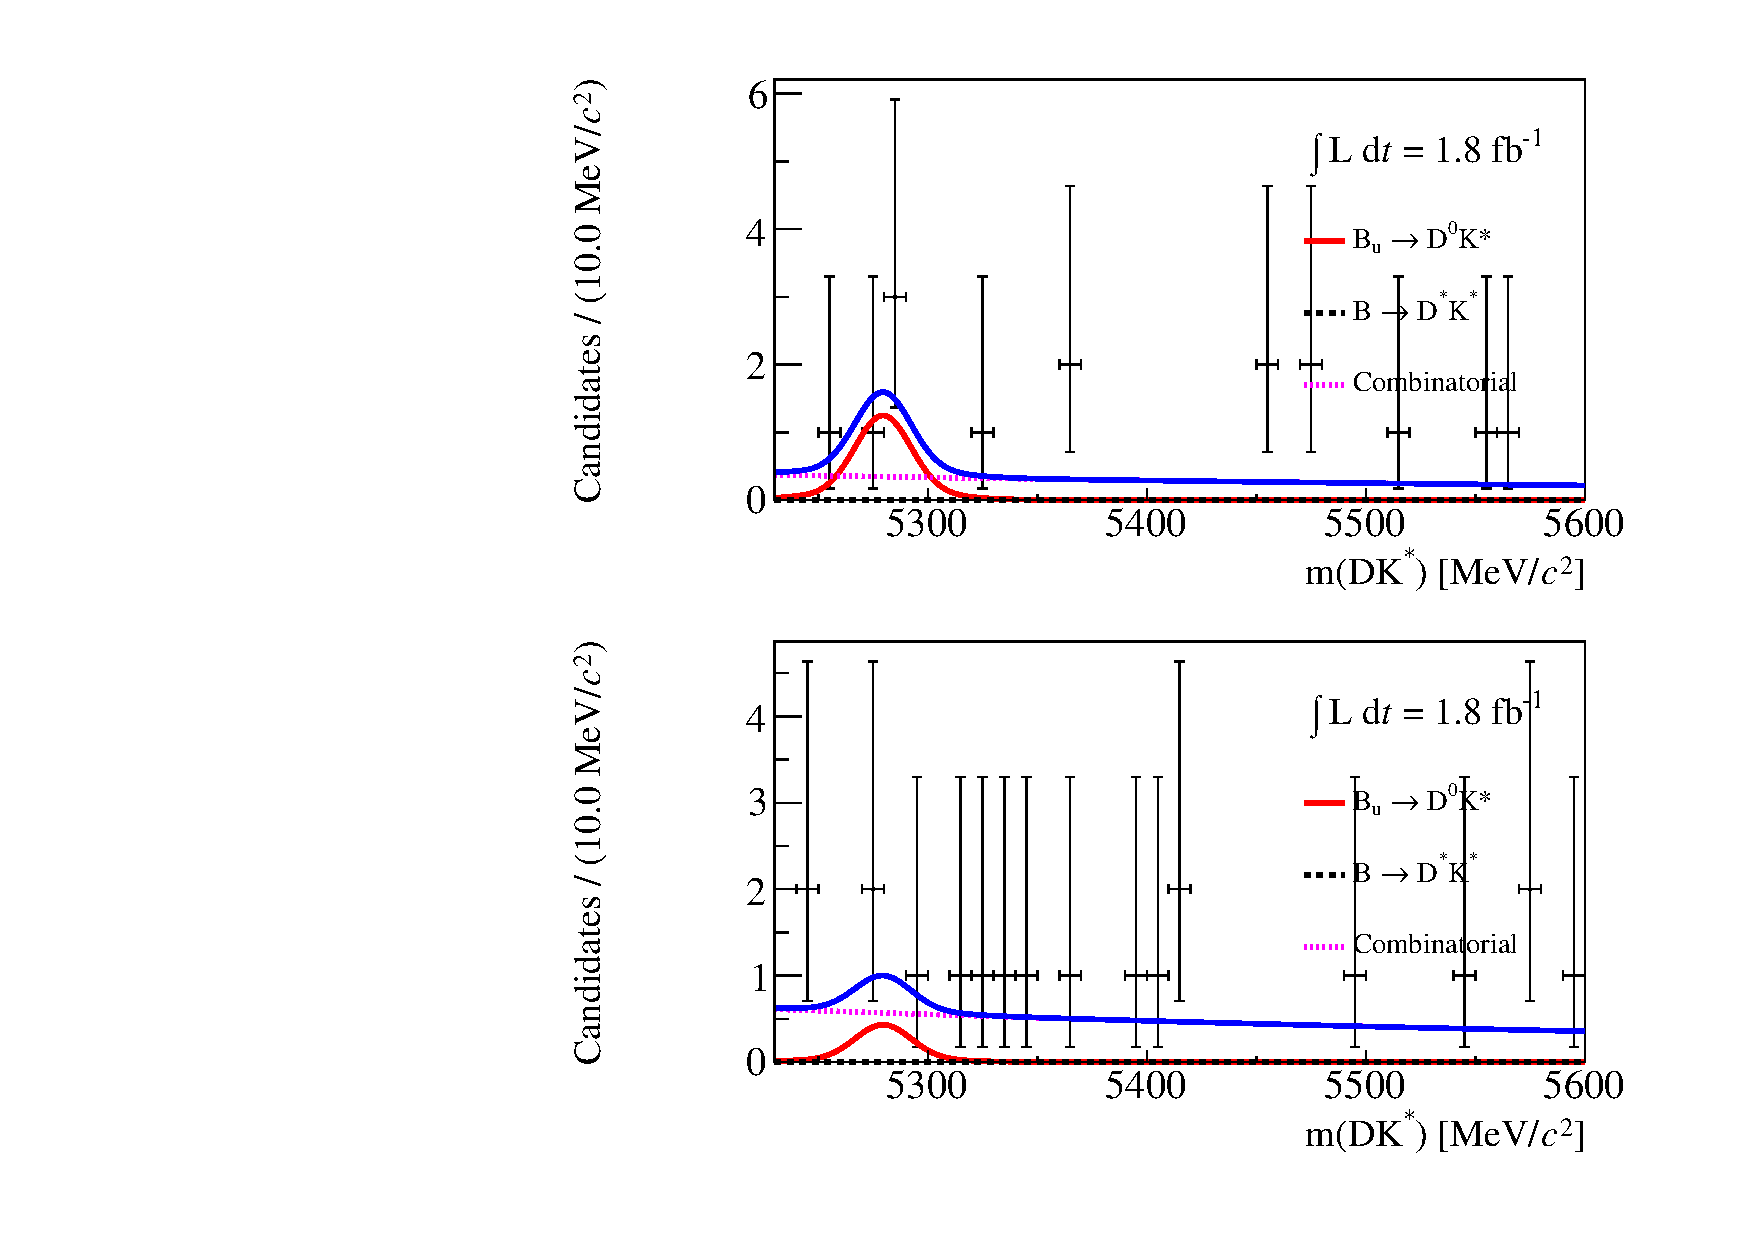
\includegraphics[width=0.3\linewidth]{figures/results/canvas_d2pikpipi_DD_run2.pdf}}
\caption{Results of the simultaneous fit for Run 1 data for 4-body modes. In each pair the top plot is for \Bp decays and the bottom plot is for \Bm decays.}
\label{datafit4bodyRun2}
\end{sidewaysfigure}

\begin{table}[h]
\centering
{\footnotesize
\begin{tabular}{cccc}
Parameter & Fitted value & Negative error & Positive error \\
\hline
$A_{K\pi}$ & $-0.004$ & $-0.023$ & $0.023$ \\
$A_{KK}$ & $0.06$ & $-0.07$ & $0.07$ \\
$A_{\pi\pi}$ & $0.15$ & $-0.13$ & $0.13$ \\
$R_{KK}$ & $1.24$ & $-0.08$ & $0.09$ \\
$R_{\pi\pi}$ & $1.08$ & $-0.14$ & $0.15$ \\
$R^+_{K\pi}$ & $0.020$ & $-0.006$ & $0.006$ \\
$R^-_{K\pi}$ & $0.0018$ & $-0.0032$ & $0.0040$ \\
$A_{K\pi\pi\pi}$ & $-0.013$ & $-0.031$ & $0.031$ \\
$A_{\pi\pi\pi\pi}$ & $0.03$ & $-0.11$ & $0.11$ \\
$R_{\pi\pi\pi\pi}$ & $1.11$ & $-0.12$ & $0.13$ \\
$R^+_{K\pi\pi\pi}$ & $0.016$ & $-0.006$ & $0.008$ \\
$R^-_{K\pi\pi\pi}$ & $0.006$ & $-0.005$ & $0.006$ \\
\end{tabular}}
\caption{Fitted values of all the physics parameters from the \CP fit}
\label{cpfitresultsphysics}
\end{table}

\begin{table}[h]
\centering
{\footnotesize
\begin{tabular}{cccc}
Parameter & Fitted value & Negative error & Positive error \\
\hline
N\_d2kpi\_DD\_run1 & $503$ & $-22$ & $23$ \\
N\_d2kpi\_DD\_run2 & $911$ & $-32$ & $32$ \\
N\_d2kpi\_LL\_run1 & $228$ & $-14$ & $15$ \\
N\_d2kpi\_LL\_run2 & $388$ & $-19$ & $19$ \\
N\_d2kpipipi\_DD\_run1 & $233$ & $-15$ & $16$ \\
N\_d2kpipipi\_DD\_run2 & $560$ & $-26$ & $26$ \\
N\_d2kpipipi\_LL\_run1 & $101$ & $-9$ & $10$ \\
N\_d2kpipipi\_LL\_run2 & $251$ & $-16$ & $16$ \\
bu\_mean\_kpi & $5279.4$ & $-0.3$ & $0.3$ \\
bu\_mean\_kpipipi & $5279.5$ & $-0.5$ & $0.5$ \\
bu\_width\_kpi & $12.1$ & $-0.3$ & $0.3$ \\
bu\_width\_kpipipi & $12.6$ & $-0.4$ & $0.4$ \\
exp\_kpi\_DD\_combs\_slope & $-0.0008$ & $-0.0006$ & $0.0006$ \\
exp\_kpi\_LL\_combs\_slope & $0.0002$ & $-0.0011$ & $0.0012$ \\
exp\_kpipipi\_DD\_combs\_slope & $-0.0014$ & $-0.0006$ & $0.0006$ \\
exp\_kpipipi\_LL\_combs\_slope & $-0.0003$ & $-0.0014$ & $0.0015$ \\
\end{tabular}}
\caption{Fitted values of the signal yields and shape parameters from the \CP fit}
\label{cpfitresultsshapes}
\end{table}

Table \ref{cpfitresultscomb} shows the fit results for all the combintoric yields.

\begin{table}[h]
\centering
{\tiny
\begin{tabular}{cccc}
Parameter & Fitted value & Negative error & Positive error \\
\hline
n\_comb\_d2kk\_minus\_DD\_run1 & $9.2644$ & $-3.2413$ & $4.1306$ \\
n\_comb\_d2kk\_minus\_DD\_run2 & $29.5912$ & $-5.8248$ & $6.6312$ \\
n\_comb\_d2kk\_minus\_LL\_run1 & $0.0000$ & $0.0000$ & $0.8409$ \\
n\_comb\_d2kk\_minus\_LL\_run2 & $10.2769$ & $-3.2586$ & $4.0635$ \\
n\_comb\_d2kk\_plus\_DD\_run1 & $11.0377$ & $-3.2611$ & $4.0359$ \\
n\_comb\_d2kk\_plus\_DD\_run2 & $28.5043$ & $-5.6729$ & $6.4917$ \\
n\_comb\_d2kk\_plus\_LL\_run1 & $6.9477$ & $-2.7573$ & $3.6031$ \\
n\_comb\_d2kk\_plus\_LL\_run2 & $4.1843$ & $-1.9720$ & $2.8582$ \\
n\_comb\_d2kpi\_minus\_DD\_run1 & $54.6504$ & $-8.3230$ & $9.2240$ \\
n\_comb\_d2kpi\_minus\_DD\_run2 & $155.8847$ & $-14.5137$ & $15.4315$ \\
n\_comb\_d2kpi\_minus\_LL\_run1 & $7.9888$ & $-2.8410$ & $3.7060$ \\
n\_comb\_d2kpi\_minus\_LL\_run2 & $15.9239$ & $-4.2968$ & $5.2111$ \\
n\_comb\_d2kpi\_plus\_DD\_run1 & $64.6413$ & $-9.1168$ & $10.0035$ \\
n\_comb\_d2kpi\_plus\_DD\_run2 & $154.8678$ & $-14.5472$ & $15.4779$ \\
n\_comb\_d2kpi\_plus\_LL\_run1 & $13.0412$ & $-3.8827$ & $4.7734$ \\
n\_comb\_d2kpi\_plus\_LL\_run2 & $19.8632$ & $-4.8676$ & $5.7870$ \\
n\_comb\_d2kpipipi\_minus\_DD\_run1 & $43.3016$ & $-7.2924$ & $8.1779$ \\
n\_comb\_d2kpipipi\_minus\_DD\_run2 & $135.8805$ & $-13.5205$ & $14.4923$ \\
n\_comb\_d2kpipipi\_minus\_LL\_run1 & $1.2423$ & $-0.8669$ & $1.6936$ \\
n\_comb\_d2kpipipi\_minus\_LL\_run2 & $9.5762$ & $-3.1916$ & $4.1240$ \\
n\_comb\_d2kpipipi\_plus\_DD\_run1 & $26.9317$ & $-5.7903$ & $6.6844$ \\
n\_comb\_d2kpipipi\_plus\_DD\_run2 & $99.1967$ & $-11.8452$ & $12.8635$ \\
n\_comb\_d2kpipipi\_plus\_LL\_run1 & $3.2506$ & $-1.7378$ & $2.6474$ \\
n\_comb\_d2kpipipi\_plus\_LL\_run2 & $13.2367$ & $-3.9555$ & $4.9514$ \\
n\_comb\_d2pik\_minus\_DD\_run1 & $4.9988$ & $-1.9166$ & $2.5806$ \\
n\_comb\_d2pik\_minus\_DD\_run2 & $22.0339$ & $-4.6793$ & $5.3881$ \\
n\_comb\_d2pik\_minus\_LL\_run1 & $5.7087$ & $-2.1669$ & $2.8313$ \\
n\_comb\_d2pik\_minus\_LL\_run2 & $8.7460$ & $-2.6869$ & $3.3592$ \\
n\_comb\_d2pik\_plus\_DD\_run1 & $3.5811$ & $-1.7805$ & $2.5381$ \\
n\_comb\_d2pik\_plus\_DD\_run2 & $18.5923$ & $-4.4531$ & $5.1798$ \\
n\_comb\_d2pik\_plus\_LL\_run1 & $6.2716$ & $-2.3435$ & $3.0760$ \\
n\_comb\_d2pik\_plus\_LL\_run2 & $10.1699$ & $-3.0098$ & $3.7295$ \\
n\_comb\_d2pikpipi\_minus\_DD\_run1 & $2.3189$ & $-1.2711$ & $1.9952$ \\
n\_comb\_d2pikpipi\_minus\_DD\_run2 & $17.6630$ & $-4.0703$ & $4.7570$ \\
n\_comb\_d2pikpipi\_minus\_LL\_run1 & $2.8918$ & $-1.4152$ & $2.0824$ \\
n\_comb\_d2pikpipi\_minus\_LL\_run2 & $8.0364$ & $-2.7499$ & $3.4109$ \\
n\_comb\_d2pikpipi\_plus\_DD\_run1 & $8.5916$ & $-2.7559$ & $3.4576$ \\
n\_comb\_d2pikpipi\_plus\_DD\_run2 & $11.3239$ & $-3.2068$ & $3.9408$ \\
n\_comb\_d2pikpipi\_plus\_LL\_run1 & $0.5468$ & $0.0000$ & $1.5795$ \\
n\_comb\_d2pikpipi\_plus\_LL\_run2 & $8.1112$ & $-2.7664$ & $3.5289$ \\
n\_comb\_d2pipi\_minus\_DD\_run1 & $2.5555$ & $-1.3991$ & $2.1909$ \\
n\_comb\_d2pipi\_minus\_DD\_run2 & $22.3622$ & $-5.1858$ & $6.0198$ \\
n\_comb\_d2pipi\_minus\_LL\_run1 & $2.8497$ & $-1.5111$ & $2.2778$ \\
n\_comb\_d2pipi\_minus\_LL\_run2 & $4.5092$ & $-1.8921$ & $2.6286$ \\
n\_comb\_d2pipi\_plus\_DD\_run1 & $6.3000$ & $-2.4807$ & $3.2589$ \\
n\_comb\_d2pipi\_plus\_DD\_run2 & $20.7800$ & $-4.7887$ & $5.5926$ \\
n\_comb\_d2pipi\_plus\_LL\_run1 & $1.2180$ & $-0.8483$ & $1.6131$ \\
n\_comb\_d2pipi\_plus\_LL\_run2 & $4.4715$ & $-1.9438$ & $2.6960$ \\
n\_comb\_d2pipipipi\_minus\_DD\_run1 & $6.4229$ & $-2.4483$ & $3.2700$ \\
n\_comb\_d2pipipipi\_minus\_DD\_run2 & $39.6563$ & $-6.6510$ & $7.4336$ \\
n\_comb\_d2pipipipi\_minus\_LL\_run1 & $4.4140$ & $-1.9854$ & $2.7711$ \\
n\_comb\_d2pipipipi\_minus\_LL\_run2 & $14.1558$ & $-3.8758$ & $4.6747$ \\
n\_comb\_d2pipipipi\_plus\_DD\_run1 & $8.7170$ & $-3.0106$ & $3.8208$ \\
n\_comb\_d2pipipipi\_plus\_DD\_run2 & $38.6850$ & $-6.5763$ & $7.3661$ \\
n\_comb\_d2pipipipi\_plus\_LL\_run1 & $3.0998$ & $-1.4649$ & $2.1490$ \\
n\_comb\_d2pipipipi\_plus\_LL\_run2 & $9.5359$ & $-3.1792$ & $4.0340$ \\
\end{tabular}}
\caption{Fitted values of all the combinatoric yields from the \CP fit}
\label{cpfitresultscomb}
\end{table}

\begin{table}
\centering
\begin{tabular}{c|c}
\hline
\D mode & Total yield \\
\hline
$K\pi$ & $2030 \pm 49$ \\
$KK$ & $257 \pm 18$ \\
$\pi\pi$ & $80 \pm 11$ \\
$\pi K$ & $20 \pm 7$ \\
$K\pi\pi\pi$ & $1144 \pm 37$ \\
$\pi\pi\pi\pi$ & $115 \pm 13$ \\
$\pi K\pi\pi$ & $13 \pm 7$ \\
\hline
\end{tabular}
\caption{Total fitted yields in each of the \D decay modes from the charge combined fit}
\label{fittedyields}
\end{table}


%%%%%%%%%%%%%%%%%%%%%%%%

\clearpage

\section{Systematics}
\label{sec:systematics}

In this section, various sources of systematic uncertainty that affect the measurement are investigated. Many fixed parameters are used in the fit model and each need to be assigned a systematic uncertainty. Systematics are computed either by multiple fits to data with certain parameters smeared or in a toy setup where the generation is different to the fit model. 

\subsection{Sources of systematic uncertainty}

The branching ratios, MC efficiencies, PID efficiencies, veto efficiencies, and production, detection and PID asymmetries all have associated systematic uncertainties. These are estimated by performing multiple fits to data where the relevant fixed parameter are varied according to a Gaussian whose width is the assigned uncertainty. For each fit observable a histogram is created containing the results for each data fit, the RMS of this histogram is taken to be the systematic uncertainty for this parameter.

Signal shape, partially reconstructed contribution, combinatoric shape and charmless contribution all all have associated systematic uncertainties. These are computed using a toy setup where the generated model is different to the fit model. The systematic is taken to be the difference between the mean of the fitted distribution and the generated value.

\subsubsection{Branching ratios}

The branching ratios for the different \D decays are used in the \CP fit as shown in Equations \ref{effcorrectionglw2body} and \ref{effcorrectionglw4body}. The values used for the branching ratios are given in Table \ref{fitinputs} along with their uncertainties~\cite{PDG2014}. A systematic is assigned by performing 1000 fits to data each time varying the branching ratio values by a Gaussian with a width corresponding to the uncertainty of each branching ratio.

\subsubsection{MC efficiencies}

Selection efficincies and BDT efficiencies are used in the \CP fit as shown in Equations \ref{effcorrectionglw2body}, \ref{effcorrectionglw4body}, \ref{effcorrectionads2body} and \ref{effcorrectionads4body}. The values used in the \CP fit are shown in Table \ref{fitinputs} along with their uncertainties. These values are fixed in the \CP fit. The Run 2 uncertainties are estimated assuming 2016 MC efficiencies have the same central value as 2015 but with twice the uncertainty.  A systematic is assigned by performing 1000 fits to data each time varying these fixed parameters according to a Gaussian whose width is the assigned unceratinty for that parameter.

\subsubsection{PID efficiencies}

PID efficiencies are used in the \CP fit as shown in Equations \ref{effcorrectionglw2body} and \ref{effcorrectionglw4body} and the values used are shown in Table \ref{fitinputs}. A systematic is assigned by performing 1000 fits to data each time varying the PID efficiencies according to a Gaussian whose width is the assigned unceratinty for that value.

\subsubsection{Veto efficiencies}

Veto efficiencies are required in the \CP fit to correct for the veto applied in the two- and four-body ADS modes, as shown in Equations \ref{effcorrectionads2body} and \ref{effcorrectionads4body}, with the actual values used shown in Tables \ref{fitinputs} as well as the uncertainties. The Run 2 uncertainties are estimated assuming 2016 MC efficiencies have the same central value as 2015 but with twice the uncertainty. A systematic is assigned by performing 1000 fits to data each time varying the veto efficiencies according to a Gaussian whose width is the assigned unceratinty for that value.

\subsubsection{Asymmetry corrections}

Corrections must be made in the \CP for various sources of asymmetry as detailed in Section \ref{sec:cpfit:asymmetries}, namely production asymmetry, detection asymmetry and PID asymmetry. For each source of asymmetry a correction is applied in the \CP fit and a systematic is assigned separately to each based on the uncertainty of each correction. Details of the values used with their corresponding uncertainties are given in Section \ref{sec:cpfit:asymmetries}. It is worth noting that for production asymmetry, the Run 2 value is taken to have the same central value as Run 1 with double the uncertainty. 

\subsubsection{Signal shape}
\label{sec:systematics:signal}

The signal shape, described in Section \ref{sec:massfit:signal}, is modelled as a Double Crystal Ball with all the parameters fixed from MC apart from the mean and width. From signal MC it can be seen that the signal shape has more than one characteristic width a low mass tail. There are two sources of unceratinty in the choice of signal shape: the tail parameters, $\alpha$ and $n$, and the width ratio and yield fraction, $f_{\sigma}$ and $f_{cb}$, between the two CBs. These two sources of uncertainty are treated separately and combined. The uncertainty in the tail parameters is quantified by generating 1000 toys with a Double Johnson signal shape, but fitting back with the original fit model. The Double Johnson is taken to have the same width ratio and yield fraction as the Double Crystal Ball used in the \CP fit. The results from this method are given in the first row of Table \ref{signalshapeSystematics}.

For the uncertainty in the width ratio and yield fraction, a systematic is assigned by performing 1000 fits to data each time varying the width ratio and yield fraction according to a Gaussian whose width is the assigned unceratinty for that value, which is taken from the fits to MC, as given in Table \ref{signalparameters}. The results from this method are given in the second row of Table \ref{signalshapeSystematics}.

The systematic from generating a Double Johnson distribution and that from varying the Doule Crystal Ball parameters are added in quadrature to give the total signal shape systematic.

\begin{table}[h]
\centering
{\footnotesize
\begin{tabular}{ccccccccc}
\hline
& $A_{K\pi}$ & $A_{KK}$ & $A_{\pi\pi}$ & $R_{KK}$ & $R_{\pi\pi}$ & $R^+_{K\pi}$ & $R^-_{K\pi}$ \\
\hline
Johnson & $1.1 \times 10^{-3}$ & $2.9 \times 10^{-3}$ & $1.1 \times 10^{-2}$ & $3.0 \times 10^{-3}$ & $2.6 \times 10^{-2}$ & $1.0 \times 10^{-3}$ & $1.3 \times 10^{-3}$ \\
Vary params & $2.3 \times 10^{-4}$ & $1.1 \times 10^{-3}$ & $1.4 \times 10^{-3}$ & $5.9 \times 10^{-4}$ & $4.4 \times 10^{-3}$ & $2.2 \times 10^{-4}$ & $1.1 \times 10^{-4}$ \\
\hline
Total & $1.1 \times 10^{-3}$ & $3.1 \times 10^{-3}$ & $1.1 \times 10^{-2}$ & $3.0 \times 10^{-2}$ & $2.7 \times 10^{-2}$ & $1.1 \times 10^{-3}$ & $1.3 \times 10^{-3}$ \\
\hline
\end{tabular}
\begin{tabular}{cccccc}
\hline
& $A_{K\pi\pi\pi}$ & $A_{\pi\pi\pi\pi}$ & $R_{\pi\pi\pi\pi}$ & $R^+_{K3\pi}$ & $R^-_{K3\pi}$ \\
\hline
Johnson & $1.6 \times 10^{-3}$ & $1.3 \times 10^{-3}$ & $9.8 \times 10^{-3}$ & $3.0 \times 10^{-3}$ & $3.8 \times 10^{-3}$ \\
Vary params & $4.7 \times 10^{-4}$ & $1.8 \times 10^{-3}$ & $2.5 \times 10^{-3}$ & $2.4 \times 10^{-4}$ & $1.2 \times 10^{-4}$ \\
\hline
Total & $1.7 \times 10^{-3}$ & $2.2 \times 10^{-3}$ & $1.0 \times 10^{-2}$ & $3.0 \times 10^{-3}$ & $3.8 \times 10^{-3}$ \\
\hline
\end{tabular}}
\caption{Summary of systematic uncertainties associated with the signal shape}
\label{signalshapeSystematics}
\end{table}

\subsubsection{Combinatoric}

The shape of the combinatoric is fixed across all \D modes, the statistics are not enough to have the shapes floating. In order to get an idea of the variation in combinatoric shape between different \D modes, fits are performed to the high B mass region (5400 - 5600 \mevcc) using an exponential as the fit model, as shown in Figures \ref{combinatoricLL} and \ref{combinatoricDD}. The data used for these fits is Run 1 data with stripping and pre-selection applied, except for \Kstar selection and \Dz and \KS FD significance cuts. PID selection on the \D daughters is also applied in order to be sure of accessing the difference between the different \D modes. The full selection was not applied as there is not enough statistics to perform a meaningful fit.

\begin{figure}[h]
\centering
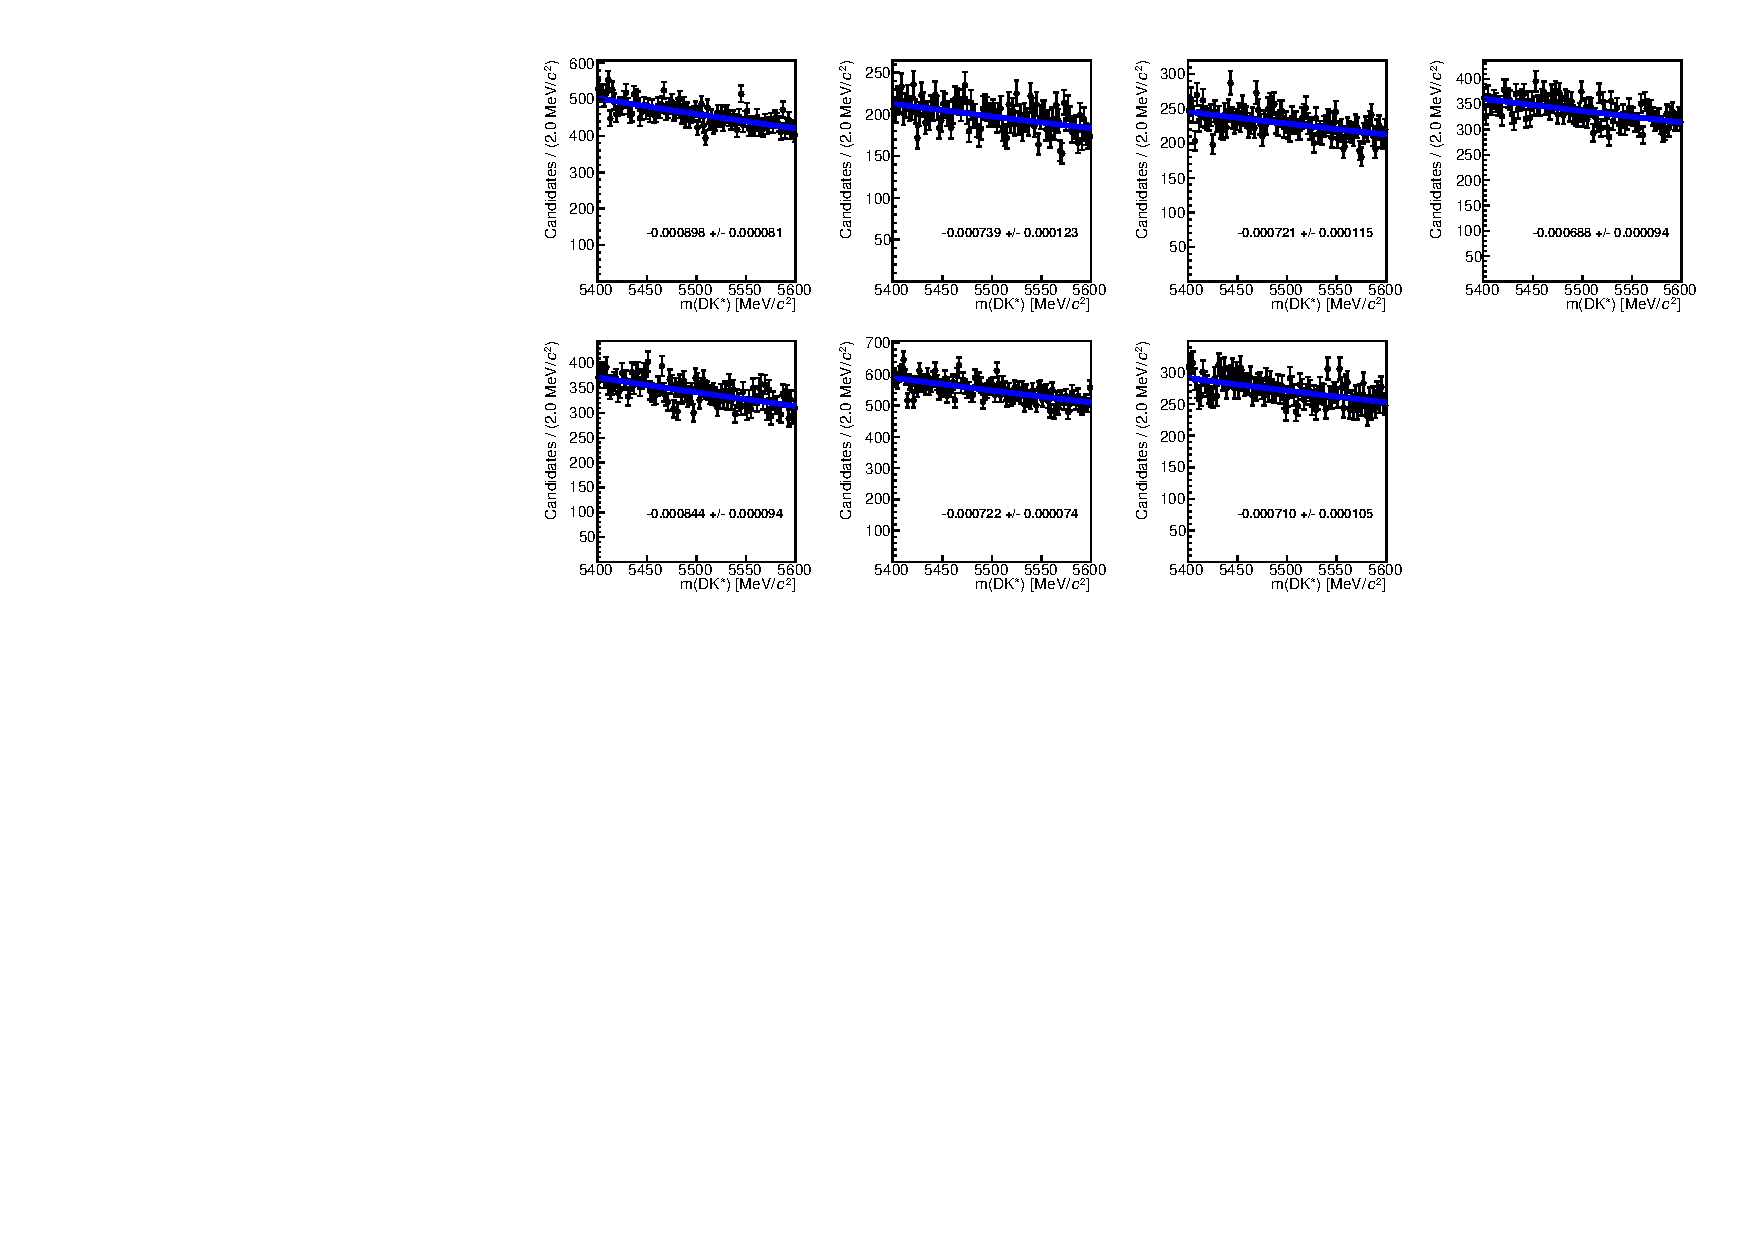
\includegraphics[width=\linewidth]{figures/fitComponents/combinatoricFits_LL.pdf}
\caption{Fits to the combinatoric background in the high B mass region for LL candidates. The fitted values for the exponential slope parameter are given on each plot}
\label{combinatoricLL}
\end{figure}

\begin{figure}[h]
\centering
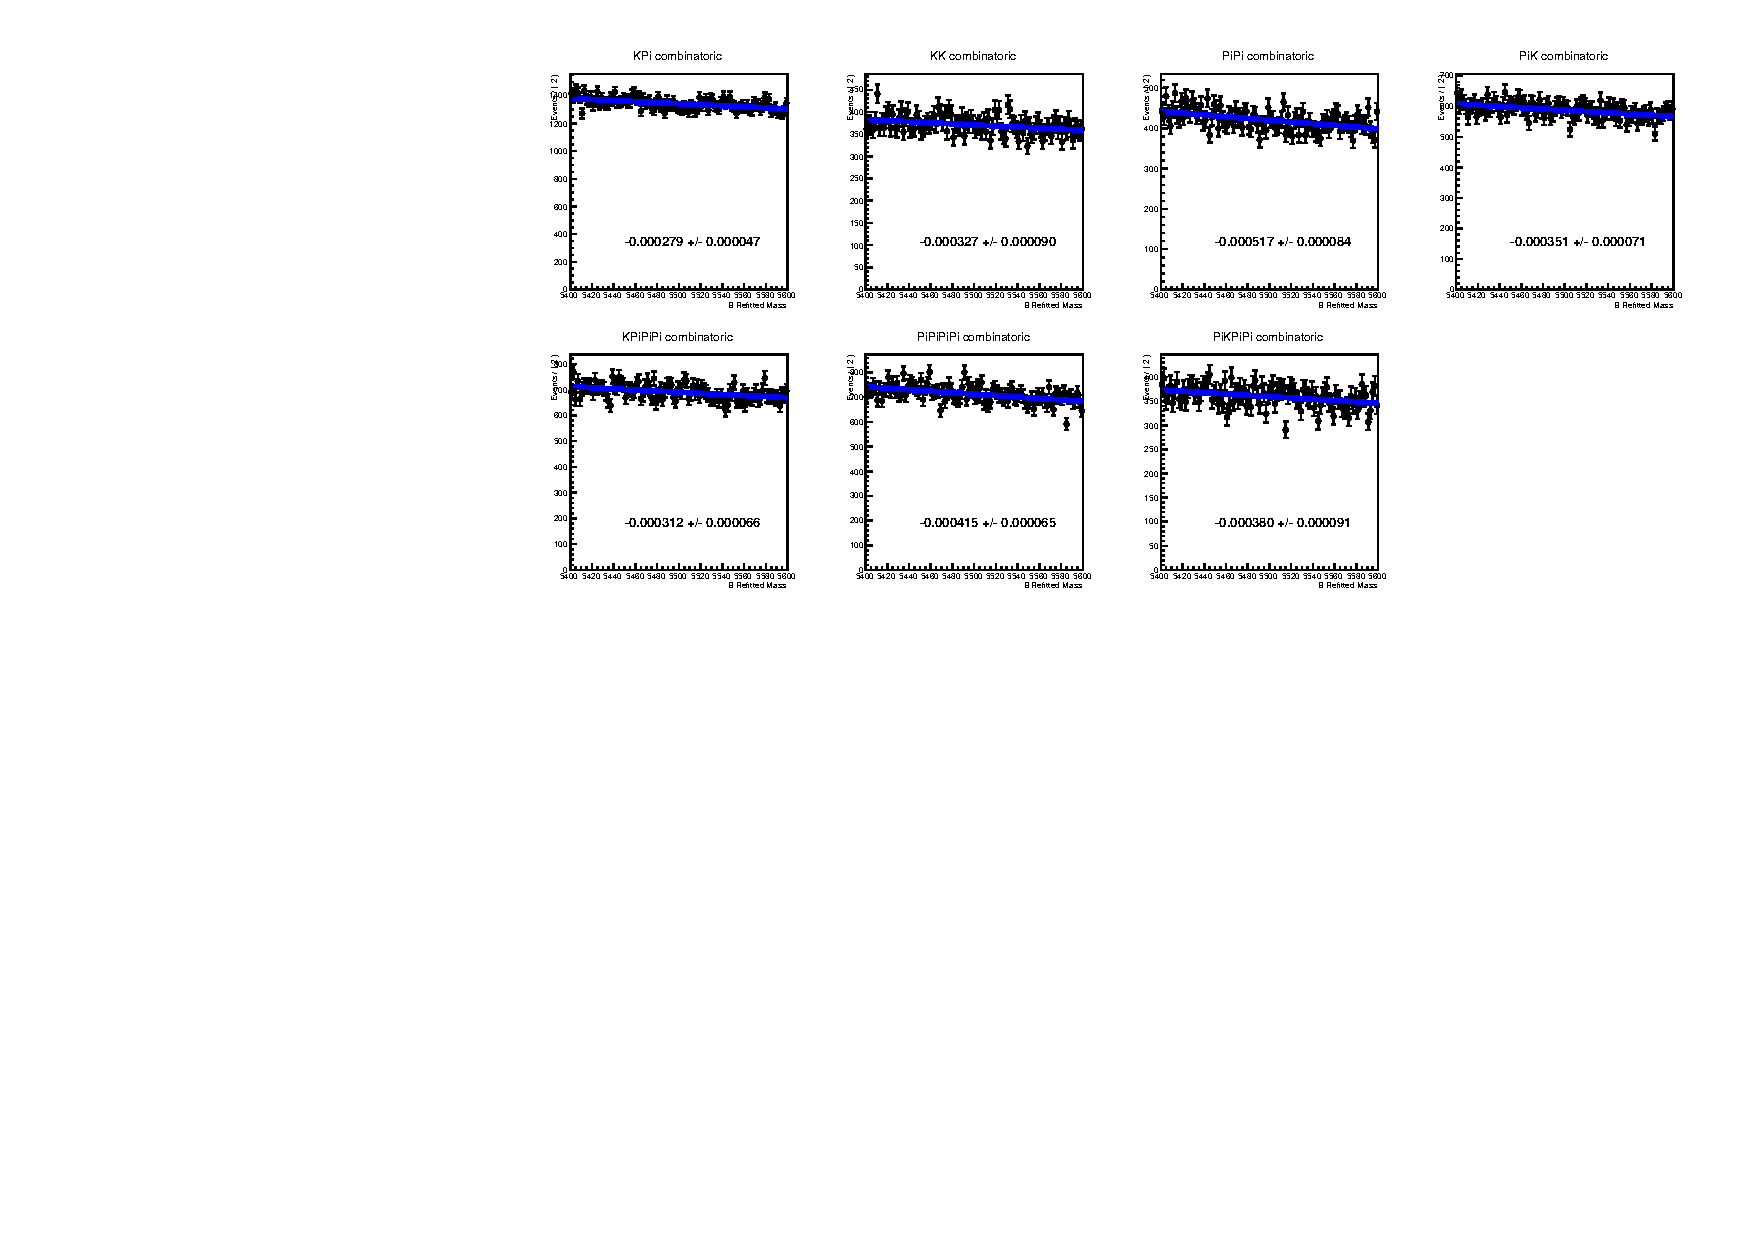
\includegraphics[width=\linewidth]{figures/fitComponents/combinatoricFits_DD.pdf}
\caption{Fits to the combinatoric background in the high B mass region for DD candidates. The fitted values for the exponential slope parameter are given on each plot}
\label{combinatoricDD}
\end{figure}

The systematic is assigned by generating 1000 toys with the combinatoric shape parameter for each mode fixed to those given in Figures \ref{combinatoricLL} and \ref{combinatoricDD}, but fitting back with the original fit model.

\subsubsection{Partially reconstructed}
\label{sec:systematics:partreco}

The partially reconstructed decays have a completely fixed shape and yield contributing to the \CP fit. The shape parameters are fixed from fits to MC, yield ratios are fixed from branching ratios and MC efficiencies and total yield is fixed from the fit to $K\pi$ invariant mass. The estimated yield is divided equally between \Bp and \Bm bins. In order to assign a systematic three different modifications are made to the partially reconstructed region:

\begin{itemize}
\item The yield is incrased by 20\%. The uncertainty in the yield from the fit to $K\pi$ invariant mass is about 5\%, but this is considered to be an underestimate, therefore a conservative systematic of 20\% is used
\item All partially reconstructed shape are smeared by the difference in signal width between MC and data. The width for all partially reconstructed shapes is increased by 4\% of LL bins and 5\% for DD bins
\item A 10\% asymmetry is introduced for the partially reconstructed shapes
\end{itemize}

These adjustments are applied simultaneously. The systematic is assigned by generating 1000 toys with the above modifications implemented, but fitting back with the original fit model.

\subsubsection{Charmless}

Section \ref{sec:backgrounds:charmless} shows that there is a possibility for residual charmless contribution in \decay{\D}{\pi\pi} mode. Charmless events in the $\pi\pi$ mode were generated according to a Gaussian whose mean is the expected number of charmless events and the width is the corresponding unceratinty, as given in Tables \ref{charmlessyields} and \ref{charmlessyieldsRun2}. This value is rounded to a whole number and randomly distributed between \Bp and \Bm as a component of the yield in the signal region. The systematic is assigned by generating 1000 toys with a charmless contrbution introduced, but fitting back with the original fit model.

\subsection{Results of systematic uncertainties}

Table \ref{systematics} summarises the systematics for various different sources. If the systematic unceratinty was found to be more than 2 orders of magntiude smaller than the statistical unceratinty then a value of zero is given. Systematics from MC efficiencies and branching ratios mainly affects $R_{KK}$ and $R_{\pi\pi}$. Production and detection asymmetry systematics contribute to $A_{K\pi}$, $A_{KK}$ and $A_{\pi\pi}$. PID efficiencies and PID asymmetry correction do not contribute much to the systematic uncertainty. The signal shape systematic have a non-negligible effect on the uncertainty for all the physics observables. All systematic uncertainties are smaller than the corresponding statistical uncertainty. 

\begin{sidewaystable}
\centering
{\footnotesize
\begin{tabular}{ccccccccccccc}
\hline
& $A_{K\pi}$ & $A_{KK}$ & $A_{\pi\pi}$ & $R_{KK}$ & $R_{\pi\pi}$ & $R^+_{K\pi}$ & $R^-_{K\pi}$ & $A_{K\pi\pi\pi}$ & $A_{\pi\pi\pi\pi}$ & $R_{\pi\pi\pi\pi}$ & $R^+_{K3\pi}$ & $R^-_{K3\pi}$ \\
\hline
Statistical & $0.023$ & $0.07$ & $0.13$ & $0.09$ & $0.15$ & $0.006$ & $0.004$ & $0.031$ & $0.11$ & $0.13$ & $0.008$ & $0.007$ \\
\hline
BRs  & $0.0$ & $0.0$ & $0.013$ & $0.001$ & $0.012$ & $0.0$ & $0.0$ & $0.0$ & $0.0008$ & $0.027$ & $0.0$ & $0.0$ \\
MC efficiencies  & $0.0$ & $0.0$ & $0.007$ & $0.0$ & $0.006$ & $0.0002$ & $0.0$ & $0.0$ & $0.0005$ & $0.010$ & $0.0$ & $0.0$ \\
PID efficiencies  & $0.0$ & $0.0$ & $0.002$ & $0.0$ & $0.002$ & $0.0$ & $0.0$ & $0.0$ & $0.0$ & $0.003$ & $0.0$ & $0.0$ \\
Veto efficiencies  & $0.0$ & $0.0$ & $0.0$ & $0.0$ & $0.0$ & $0.0001$ & $0.0$ & $0.0$ & $0.0$ & $0.0$ & $0.0$ & $0.0$ \\
$A_{prod}$  & $0.0073$ & $0.007$ & $0.0$ & $0.008$ & $0.0$ & $0.0$ & $0.0$ & $0.0079$ & $0.0077$ & $0.0$ & $0.0$ & $0.0$ \\
$A_{det}$  & $0.0034$ & $0.003$ & $0.0$ & $0.003$ & $0.0$ & $0.0001$ & $0.0$ & $0.0034$ & $0.0030$ & $0.0$ & $0.0001$ & $0.0$ \\
$A_{pid}$ & $0.0$ & $0.0$ & $0.0$ & $0.0$ & $0.0$ & $0.0$ & $0.0$ & $0.0$ & $0.0$ & $0.0$ & $0.0$ & $0.0$ \\
Signal shape & $0.0011$ & $0.003$ & $0.011$ & $0.030$ & $0.027$ & $0.0011$ & $0.0013$ & $0.0017$ & $0.0022$ & $0.010$ & $0.0030$ & $0.0038$ \\
Combinatoric shape  & $0.0012$ & $0.003$ & $0.004$ & $0.005$ & $0.009$ & $0.0002$ & $0.0003$ & $0.0001$ & $0.0018$ & $0.0$ & $0.0012$ & $0.0004$ \\
Partially reconstructed shape  & $0.0007$ & $0.001$ & $0.001$ & $0.003$ & $0.005$ & $0.0$ & $0.0003$ & $0.0003$ & $0.0005$ & $0.002$ & $0.0008$ & $0.0001$ \\
Charmless  & $0.0008$ & $0.0$ & $0.002$ & $0.003$ & $0.007$ & $0.0$ & $0.0003$ & $0.0009$ & $0.0030$ & $0.002$ & $0.0008$ & $0.0001$ \\
\hline
Total & $0.0083$ & $0.009$ & $0.019$ & $0.012$ & $0.032$ & $0.0011$ & $0.0014$ & $0.0088$ & $0.0093$ & $0.031$ & $0.0034$ & $0.0038$ \\
\hline
\end{tabular}}
\caption{Summary of systematic uncertainties}
\label{systematics}
\end{sidewaystable}

\section{Summary of results}
\label{sec:cpfit:summary}

The \CP oberservables measured from the fit are below, where the first errors are statistical and the second are systematic.

\begin{align*}
A_{K\pi} & = -0.004 \pm 0.023 \pm 0.008 \\
A_{KK} & = 0.06 \pm 0.07 \pm 0.01 \\
A_{\pi\pi} & = 0.15 \pm 0.13 \pm 0.02 \\
R_{KK} & = 1.24 \pm 0.09 \pm 0.01 \\
R_{\pi\pi} & = 1.08 \pm 0.15 \pm 0.03 \\
R^+_{K\pi} & = 0.020 \pm 0.006 \pm 0.001 \\
R^-_{K\pi} & = 0.002 \pm 0.004 \pm 0.001 \\
A_{K\pi\pi\pi} & = -0.013 \pm 0.031 \pm 0.009 \\
A_{\pi\pi\pi\pi} & = 0.03 \pm 0.11 \pm 0.01 \\
R_{\pi\pi\pi\pi} & = 1.11 \pm 0.13 \pm 0.03 \\
R^+_{K\pi\pi\pi} & = 0.016 \pm 0.008 \pm 0.003 \\
R^-_{K\pi\pi\pi} & = 0.006 \pm 0.007 \pm 0.004 \\
\end{align*}

The statistical and systematic correlation matrices for the seven physics observables in the fit are shown in Tables \ref{statisticalcorrelations} and \ref{systematiccorrelations} respectively. Combined results from the $KK$ and $\pi\pi$ modes, taking correlations into account are,
\begin{align*}
R_{CP} = 1.20 \pm 0.08 \\
A_{CP} = 0.08 \pm 0.06
\end{align*}

\begin{sidewaystable}[h]
\centering
{\footnotesize
\begin{tabular}{c|cccccccccccc} 
\hline 
& $A_{K\pi}$ & $A_{KK}$ & $A_{\pi\pi}$ & $R_{KK}$ & $R_{\pi\pi}$ & $R^+_{K\pi}$ & $R^-_{K\pi}$ & $A_{K\pi\pi\pi}$ & $A_{\pi\pi\pi\pi}$ & $R_{\pi\pi\pi\pi}$ & $R^+_{K\pi\pi\pi}$ & $R^-_{K\pi\pi\pi}$ \\ 
 \hline
$A_{K\pi}$ & 1 & 0.00020  & 0.00017  & -0.00005  & -0.0006  & 0.076  & -0.014  & 0.0000027  & -0.000021  & 0.0011  & -0.0000045  & 0.0000028  \\
$A_{KK}$ & & 1  & -0.00012  & -0.0030  & -0.000038  & -0.0011  & -0.0024  & 0.0000054  & -0.00012  & 0.000085  & 0.000004  & 0.0000032  \\
$A_{\pi\pi}$ &  &  & 1  & -0.00062  & -0.022  & -0.0019  & -0.0017  & -0.0000021  & 0.000062  & 0.0010  & 0.000016  & 0.000017  \\
$R_{KK}$ & & & & 1  & 0.064  & 0.034  & 0.014  & -0.0000029  & 0.000057  & 0.065  & 0.000087  & 0.00011  \\
$R_{\pi\pi}$ & & & & & 1  & 0.027  & 0.017  & 0.000034  & -0.00013  & 0.030  & -0.00011  & -0.000056  \\
$R^+_{K\pi}$ & & & & & & 1  & 0.020  & 0.000016  & 0.0000014  & 0.0095  & -0.000044  & -0.000033 \\
$R^-_{K\pi}$ & & & & & & & 1  & 0.000010  & 0.00018  & -0.0050  & 0.0000095  & 0.000034  \\
$A_{K\pi\pi\pi}$ & & & & & & & & 1  & -0.00048  & -0.0014  & 0.067  & -0.033  \\
$A_{\pi\pi\pi\pi}$ & & & & & & & & & 1  & 0.00085  & 0.0029  & 0.0034  \\
$R_{\pi\pi\pi\pi}$ & & & & & & & & & & 1  & 0.031  & 0.039  \\
$R^+_{K\pi\pi\pi}$ & & & & & & & & & & & 1  & 0.028  \\
$R^-_{K\pi\pi\pi}$ & & & & & & & & & & & & 1  \\
\hline 
\end{tabular}}
\caption{Statistical correlation matrix for the seven physics observables from the \CP fit to data. The matrix is symmetric so only the top half is shown.}
\label{statisticalcorrelations}
\end{sidewaystable}
\begin{sidewaystable}[h]
\centering
{\footnotesize
\begin{tabular}{c|cccccccccccc} 
\hline 
& $A_{K\pi}$ & $A_{KK}$ & $A_{\pi\pi}$ & $R_{KK}$ & $R_{\pi\pi}$ & $R^+_{K\pi}$ & $R^-_{K\pi}$ & $A_{K\pi\pi\pi}$ & $A_{\pi\pi\pi\pi}$ & $R_{\pi\pi\pi\pi}$ & $R^+_{K3\pi}$ & $R^-_{K3\pi}$ \\ 
 \hline
$A_{K\pi}$ & 1 & 0.83  & -0.0067  & 0.72  & -0.0035  & 0.0071  & -0.025  & 0.94  & 0.84  & 0.00071  & -0.011  & -0.003  \\
$A_{KK}$ &  & 1  & -0.028  & 0.65  & 0.014  & 0.014  & -0.021  & 0.83  & 0.77  & 0.0034  & -0.0029  & 0.0045  \\
$A_{\pi\pi}$ &  &  & 1  & 0.0061  & 0.014  & 0.03  & 0.016  & -0.0073  & 0.0031  & -0.019  & -0.0056  & -0.0094  \\
$R_{KK}$ & & & & 1  & -0.032  & -0.0054  & -0.02  & 0.72  & 0.68  & -0.0028  & -0.00051  & 0.011  \\
$R_{\pi\pi}$ & & & &  & 1  & 0.057  & 0.079  & -0.0092  & 0.0012  & -0.01  & -0.017  & 0.0097  \\
$R^+_{K\pi}$ & & & & &  & 1  & 0.079  & -0.0082  & 0.0037  & -0.0022  & -0.0098  & -0.0099  \\
$R^-_{K\pi}$ & & & & & &  & 1  & -0.013  & -0.0063  & -0.012  & 0.0067  & 0.03  \\
$A_{K\pi\pi\pi}$ & & & & & & &   & 1  & 0.84  & -0.005  & -0.01  & -0.015  \\
$A_{\pi\pi\pi\pi}$ & & & & & & & &   & 1  & 0.036  & 0.0053  & 0.00047  \\
$R_{\pi\pi\pi\pi}$ & & & & & & & & &   & 1  & 0.0089  & -0.0086  \\
$R^-_{K3\pi}$ & & & & & & & & & &   & 1  & 0.045  \\
$R^-_{K3\pi}$ & & & & & & & & & & &   & 1  \\
\hline 
\end{tabular}}
\caption{Systematic correlation matrix for the seven physics observables from the \CP fit to data. The matrix is symmetric so only the top half is shown.}
\label{systematiccorrelations}
\end{sidewaystable}


\clearpage

